\documentclass[pdftex,11pt,a4paper]{report}

\usepackage[dvips]{graphicx} % to include images
\usepackage{multicol}
\usepackage{cite}
\usepackage{listings}
\usepackage{url}
\usepackage{paralist}
\usepackage{versions}
\usepackage{varioref}
\usepackage{textcomp}
\usepackage{amsmath}
% hyperref and hypcap should be last! 
% (except for algorithmic, because it conflicts with hyperref)
\usepackage[breaklinks]{hyperref}
\renewcommand{\sectionautorefname}{Section}
\renewcommand{\subsectionautorefname}{Section}
\renewcommand{\subsubsectionautorefname}{Section}
\renewcommand{\vref}[1]{\autoref{#1}\vpageref{#1}}
\usepackage[all]{hypcap}
\usepackage{algorithmic}
\usepackage[center]{caption}
\hypersetup{
    colorlinks,%
    citecolor=black,%
    filecolor=black,%
    linkcolor=black,%
    urlcolor=black
}
\excludeversion{notesfornextyear}
\newcommand{\keywords}[1]{\par\addvspace\baselineskip
\noindent\keywordname\enspace\ignorespaces#1}

\lstset{                        % settings for the code listing package
language=C++,
basicstyle=\ttfamily,           % the size of the fonts that are used for the code
showspaces=false,
showstringspaces=false,
showtabs=false,
tabsize=2,
captionpos=b,                   % sets the caption-position to bottom
breaklines=true,                % sets automatic line breaking
breakatwhitespace=false,        % sets if automatic breaks should only happen at whitespace
escapeinside={\%*}{*)}          % if you want to add a comment within your code
}

\setlength{\oddsidemargin}{0.0in}
\setlength{\evensidemargin}{0.0in}
\setlength{\topmargin}{-0.25in}
\setlength{\headheight}{0in}
\setlength{\headsep}{0in}
\setlength{\textwidth}{6.5in}
\setlength{\textheight}{9.25in}
\setlength{\parindent}{0in}
\setlength{\parskip}{2mm}

% enable number by subsubsections and let them show in ToC
\setcounter{secnumdepth}{3}
\setcounter{tocdepth}{3}

\begin{document}

\title{rUNSWift Team Report 2010\\Robocup Standard Platform League}
\date{August 2010}
\author{
Adrian Ratter
\and Bernhard Hengst
\and Brad Hall
\and Brock White
\and Benjamin Vance
\and David Claridge
\and Hung Nguyen
\and Jayen Ashar
\and Stuart Robinson
\and Yanjin Zhu
}

\begin{titlepage}%
  \let\footnotesize\small
  \let\footnoterule\relax
  \let \footnote \thanks
  \null\vfil
  \begin{center}%
    \vfill
    
\includegraphics[width=4in]{figures/unsw_runswift_logo}%
    \vskip 3em%
    {\LARGE rUNSWift Team Report 2010\\Robocup Standard Platform League \par}%
    \vskip 3em%
    {\large
     \lineskip .75em%
      \begin{tabular}[t]{c}%
        Adrian Ratter
        \and Bernhard Hengst
        \and Brad Hall
        \and Brock White
        \and Benjamin Vance
        \and Claude Sammut
        \and David Claridge
        \and Hung Nguyen
        \and Jayen Ashar
        \and Maurice Pagnucco
        \and Stuart Robinson
        \and Yanjin Zhu
      \end{tabular}\par}%
      \vskip 1.5em%
      \texttt{\{adrianr,bernhardh,bradh,brockw,bvance,claude,davidc,dhung,jayen,morri,stuartr,yanjinz\}\\@cse.unsw.edu.au}%
\vfill
    {\large \today \par}%       % Set date in \large size.
\vfill
\vskip 3cm
School of Computer Science \& Engineering\\
University of New South Wales\\
Sydney 2052, Australia\\

\vfill

%\textbf{Supervisors and Assessors}\\
%\begin{multicols}{2}{

%Maurice Pagnucco\\
%K17-104A / +61 2 9385 6925\\

%Claude Sammut\\
%K17-401J / +61 2 9385 6932\\
%}
%\end{multicols}

  \end{center}\par
  \vfil\null
\thispagestyle{empty}
  \end{titlepage}%

\pagenumbering{roman}

\newpage

\begin{abstract}
RoboCup continues to inspire and motivate our research interests in cognitive robotics and machine learning, particularly layered hybrid architectures, abstraction, and high-level programming languages. The newly formed 2010 rUNSWift team for the Standard Platform League mainly includes final year undergraduate students under the supervision of  leaders who have been involved in RoboCup for many years. In 2010 the team revamped the entire code-base and  implemented a new integrated project management system. Several innovations have been introduced in vision, localisation, locomotion and behaviours. This report describes the research and development undertaken by the team in the 2009/2010 year.
\end{abstract}

\newpage
\tableofcontents
\newpage
\pagenumbering{arabic}

% main part of the report goes here
% **********************************************************************************************************
\newpage
\chapter{Introduction}

The RoboCup Standard Platform League (SPL) has been and continues to be
excellent training for the undergraduates who also make a significant
contributions towards research. The UNSW SPL teams (and previously the
Four-legged teams) have almost entirely been made up of final-year undergraduate
students, supported by faculty and research students. The 2010 rUNSWift team
includes undergraduate students: Brock White, Benjamin Vance, David Claridge,
Adrian Ratter, Stuart Robinson, and Yanjin Zhu; postgraduate students Jayen
Ashar and Hung Nguyen; faculty staff: Bernhard Hengst, Maurice Pagnucco and
Claude Sammut; Development Manager Brad Hall (see \autoref{fig-team}).

\begin{figure} [ht]
\centering
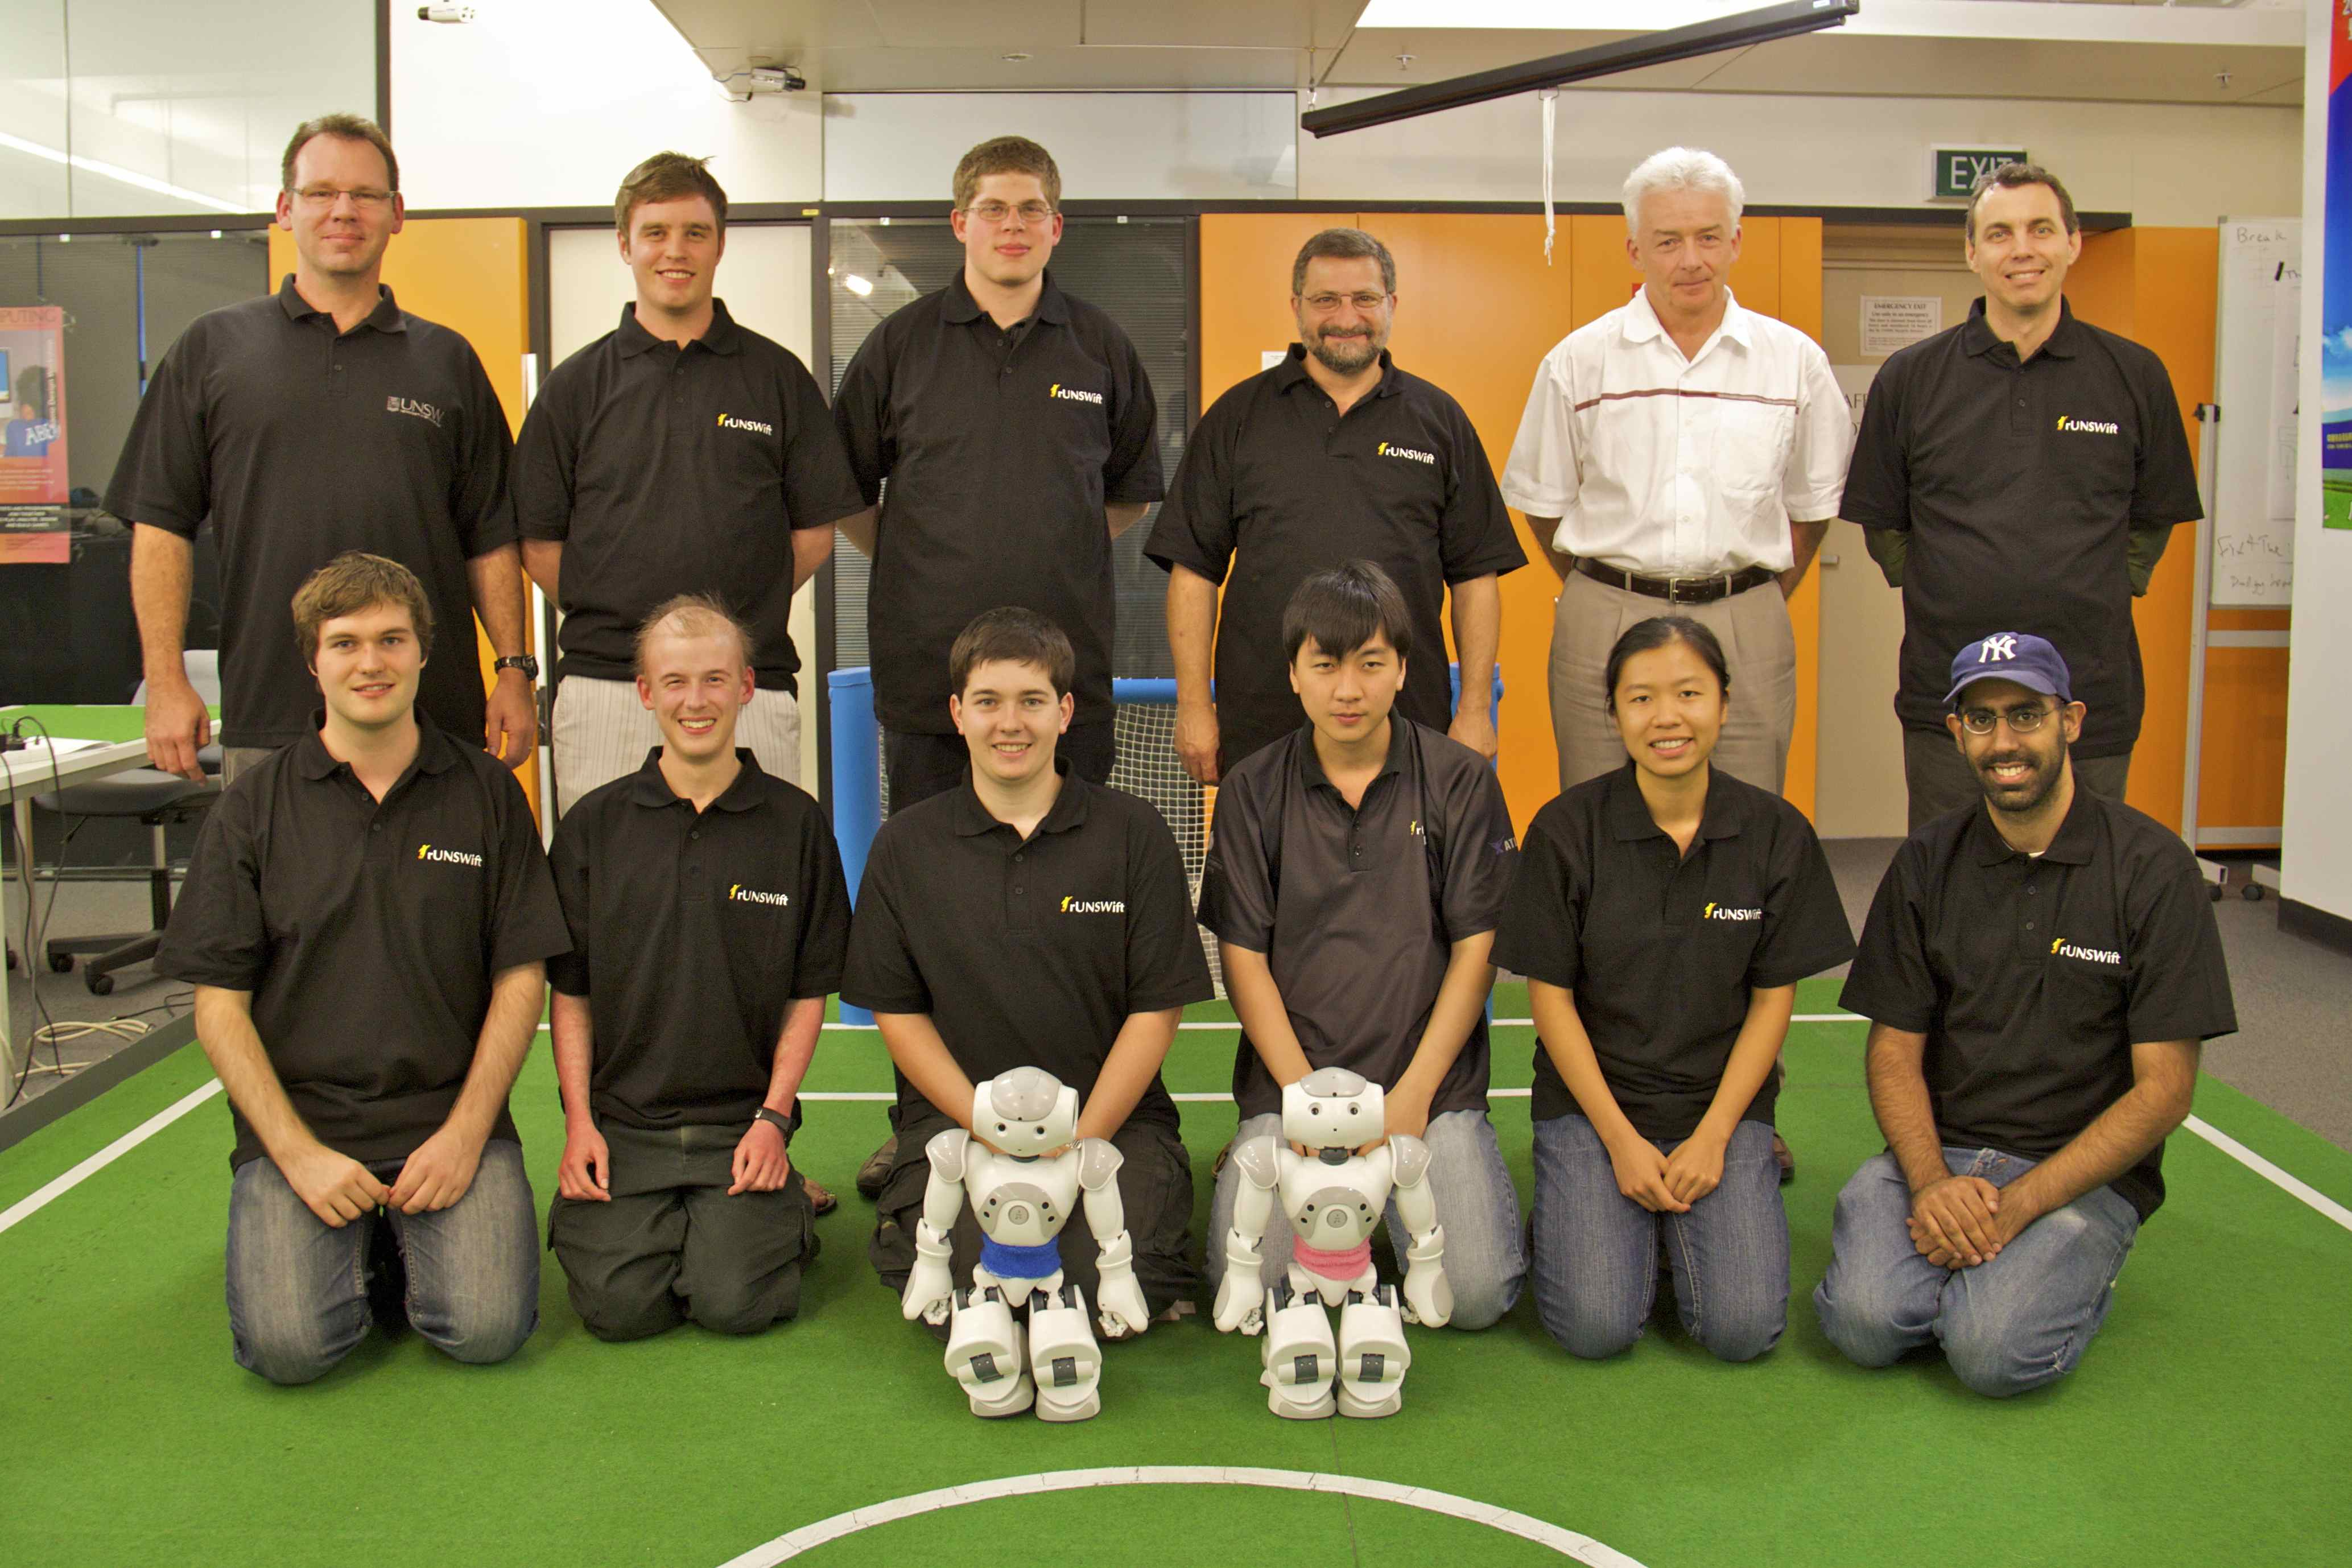
\includegraphics[width=1.0\textwidth]{figures/TeamPic.jpg}
\caption{The 2010 rUNSWift team. Left to right, top to bottom: Brad Hall, Brock White, Benjamin Vance, Claude Sammut, Bernhard Hengst, Maurice Pagnucco, David Claridge, Adrian Ratter, Stuart Robinson, Hung Nguyen, Yanjin Zhu, Jayen Ashar, Nao Blue, Nao Red.} \label{fig-team}
\end{figure}

The team has the financial support of the School of Computer Science and Engineering at UNSW and the Australian Research Council Centre of Excellence for Autonomous Systems.  The School also provides a great deal of organisational support for travel. We have a competition standard field and a wealth of experience from our participation in the four-legged league, simulation and rescue competitions. Our sponsors include Atlassian Pty Ltd.

\section{Project Management}

For 2010 we reviewed our approach to team selection, project management, supervision and research and development. We embarked on a total rewrite of the code. We have found that part-time participation by large numbers of students does not lead to coordinated deliverables. The new 2010 team has been selected on the basis that core team members devote a significant amount of their time to research and development on the SPL project and count that effort towards either their final year thesis project or an approved special project. Students are selected on the basis of academic standing and some evidence of performance on larger projects. 

\begin{figure} [t]
\centering
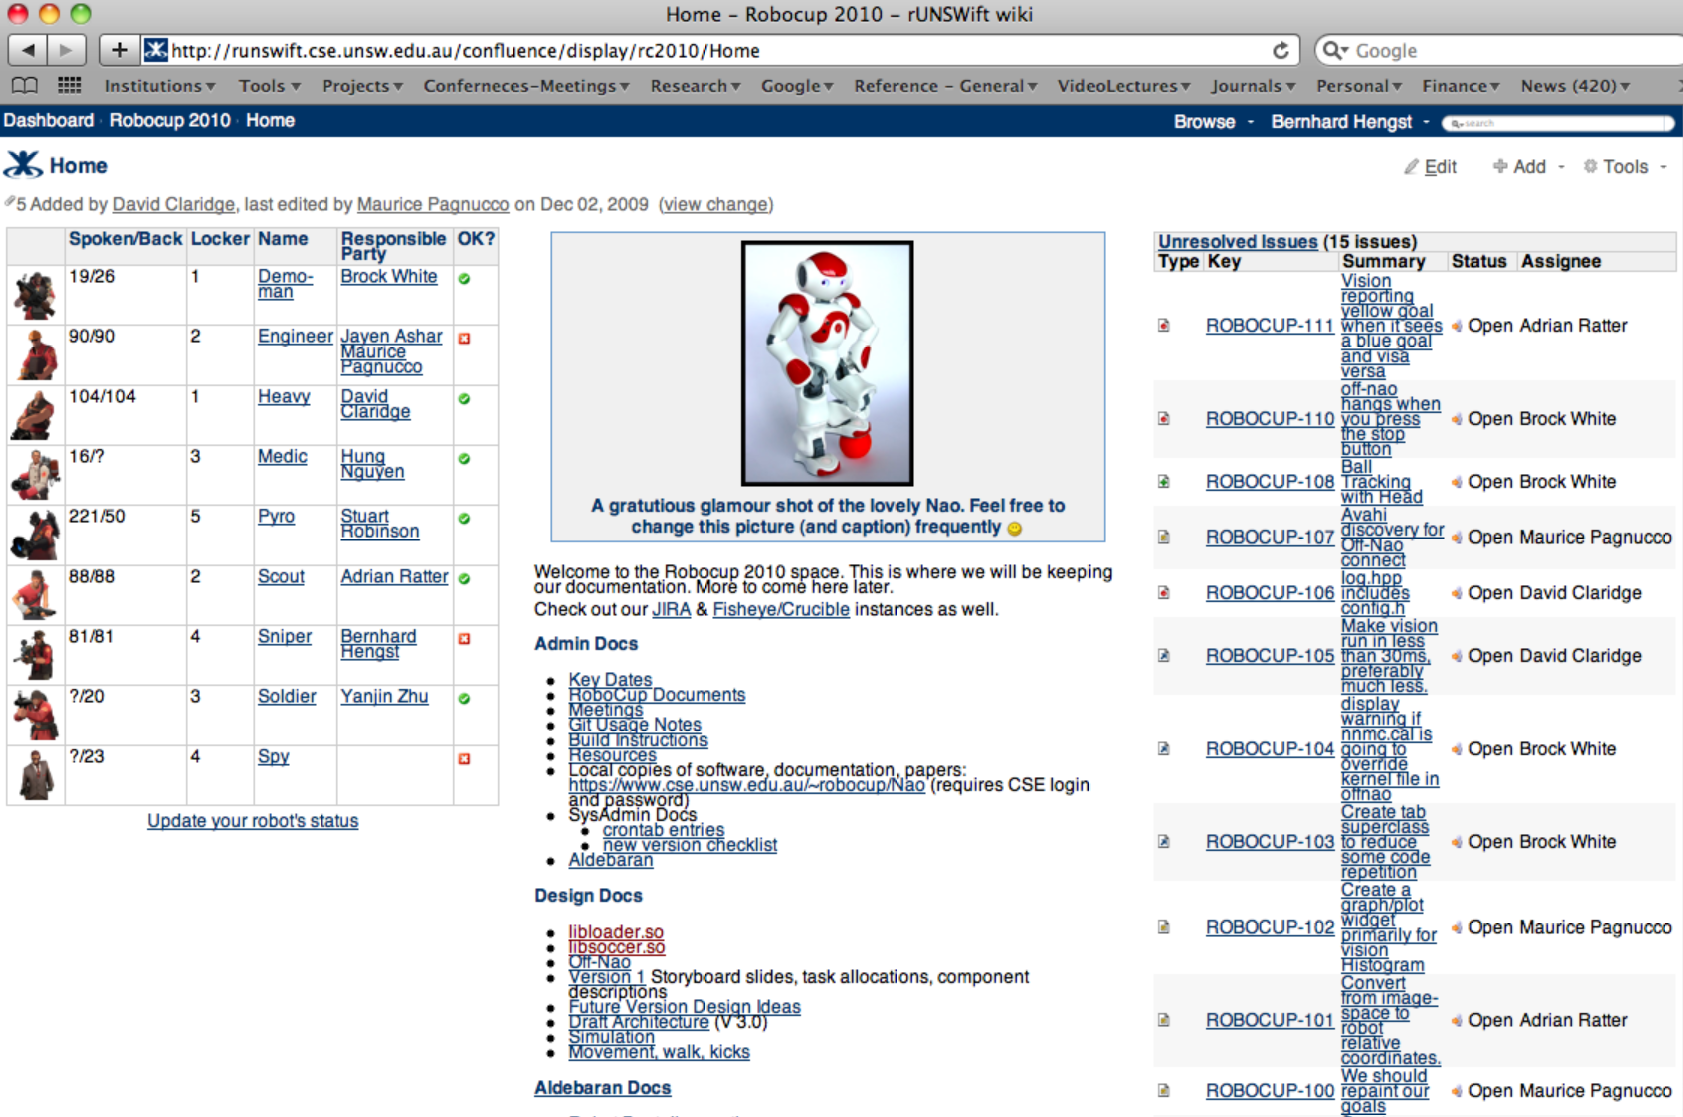
\includegraphics[width=1.0\textwidth]{figures/JIRA}
\caption{Atlassian Confluence wiki software.} \label{figJIRA}
\end{figure}

A new project management system from Atlassian Pty Ltd has been configured by the students for use by the team. The Atlassian suite of products has three components: an enterprise wiki, Confluence, is a web application that facilitates collaboration and knowledge management (see \autoref{figJIRA}); JIRA, that combines issue tracking, project management, customisable workflow to increase the velocity of software development by the team; and FishEye, that opens the source code repository to help you understand the code, facilitate code reviews and keep tabs on the team members who write it.

While many successful innovative ideas from previous years have been used to fast-track the new code, we have continued our development of a more robust vision system and non-beacon localisation. We have made some innovations in bipedal walking and the use of the foot sensors to help stabilise omni-directional locomotion. 

\section{Research Interests}

The vision of many robotics researchers is to have machines operating in unstructured, real-world environments. Our long term aim is to develop general purpose intelligent systems that can learn and be taught to perform many different tasks autonomously by interacting with their environment. As an approach to this problem, we are interested in how machines can compute abstracted representations of their environment through direct interaction, with and without human assistance, in order to achieve some objective. These future intelligent systems will be goal directed and adaptive, able to program themselves automatically by sensing and acting, accumulating knowledge over their lifetime.  

We are interested in what Cognitive Robotics can contribute to the specification of flexible behaviours. Languages such as Golog (see \cite{Levesque00legolog:inexpensive} for an application of Golog), allow the programmer to create highly reactive behaviours and the language incorporates a planner that can be invoked if the programmer wishes to be less specific about the implementation of a behaviour. 

Traditional programming languages applied to robotics require the programmer to solve all parts of the problem and result in the programmer scripting all aspects of the robot behaviour. There is no facility for planning or deliberation. As a result programs tend to be complex, unwieldy and not portable to other platforms. High level robotic languages provide a layer of abstraction that allows for a variety of programming styles from deliberative constructs that resort to AI planning in order to achieve user goals through to scripted behaviours when time critical tasks need to be completed.

Our general research focus, of which the RoboCup SPL is a part, is to:
\begin{itemize}
\item further develop reasoning methods that incorporate uncertainty and real-time constraints and that integrate with the statistical methods used in SLAM and perception
\item develop methods for using estimates of uncertainty to guide future decision making so as to reduce the uncertainty 
\item extend these methods for multi-robot cooperation
\item use symbolic representations as the basis for human-robot interaction
\item develop learning algorithms for hybrid systems, such as using knowledge of logical constraints to restrict the search of a trial-and-error learner and learning the constraints
\item develop high level symbolic robotic languages that provide abstractions for a large range of deliberation, planning and learning techniques so as to simplify robot programming
\end{itemize}

\subsection{Humanoid Robots}
Research in our group includes applications of Machine Learning to bipedal gaits. PhD student Tak Fai Yik (a member of the champion 2001 four-legged team) collaborated with Gordon Wyeth at the University of Queensland to evolve a walk for the GuRoo robot \cite{wyeth03evolving}, which was entered in the humanoid robot league. This method was inspired by the gait learning devised for the Aibos. For the humanoid, the same philosophy is applied. Starting from a parameterised gait, an optimisation algorithm searches for a set of parameter values that satisfies the optimisation criteria. In this case, the search was performed by a genetic algorithm in simulation. When a solution was found, it was transferred to the real robot, working successfully. Subsequently, the approach we used was a hybrid of a planner to suggest a plausible sequence of actions and a numerical optimisation algorithm to tune the action parameters. Thus, the qualitative reasoning of the planner provides constraints on the trial-and-error learning, reducing the number of trials required. Tak Fai developed and implemented this system for his PhD \cite{yik07locomotion}. It has been tested on a Cycloid II robot. It is our intention to continue this work as part of the development for the Nao, Bioloid and Cycloid robots.  

\subsection{Locomotion}
In 2000, rUNSWift introduced the \emph{UNSW} walk, which became the standard across the league \cite{DBLP:conf/robocup/HengstIPS01}. The key insight was to describe the trajectory of the paws by a simple geometric figure that was parameterised. This made experimentation with unusual configurations relatively easy. As a result, we were able to devise a gait that was much faster and more stable than any other team. Since then, almost all the other teams in the league have adopted a similar style of locomotion, some starting from our code.
The flexibility of this representation led to another major innovation in 2003. We were the first team to use Machine Learning to tune the robot's gait, resulting in a much faster walk \cite{Kim03automaticgait}. In succeeding years, several teams developed their own ML approaches to tuning the walk. Starting from the parameterised locomotion representation, the robots are able to measure their speed and adjust the gait parameters according to an optimisation algorithm.

\subsection{Localisation}
The 2000 competition also saw the initial use of a Kalman filter-based localisation method that continued to evolve in subsequent years \cite{DBLP:conf/robocup/PhamHIS01}. In the 2000 competition, advantages in localisation and locomotion meant that the team never scored less than 10 goals in every game and only one goal was scored against it in the entire competition. Starting from a simple Kalman filter in 2000, the localisation system evolved to include a multi-modal filter and distributed data fusion across the networked robots. In 2006, we went from treating the robots as individuals sharing information, to treating them as one team with a single calculation spread over multiple robots.  This allowed us to handle multiple hypotheses.  It also allowed us to use the ball for localisation information.

\subsection{Vision}
Our vision system evolved significantly over our eight years in the four-legged league. From the beginning, in 1999, we used a simple learning system to train the colour recognition system. In 2001, we used a standard machine learning program, C4.5, to build a decision tree recogniser. This turned out to be very important since the lighting we encountered at the competition was very different from our lab and our previous vision system was not able to cope. Also in 2000, our vision system became good enough to use robot recognition to avoid team mates \cite{DBLP:conf/isrr/SammutH01}. In later years, we updated the vision system to be much faster and to recognise field markings reliably.

\subsection{Software Engineering and Architecture}
Throughout the software development of the Aibo code, we have adopted a modular, layered architecture. The lowest layers consist of the basic operations of vision, localisation and locomotion. The behaviours of the robots are also layered, with skills such as ball tracking, go to a location, get behind ball, etc, being at the lowest level of the behaviour hierarchy, with increasingly complex behaviours composed of lower-level skills. Originally, all the behaviours were coded in C/C++ but in 2005 and 2006, as in 2010, the upper layers were replaced by Python code.  We have also experimented with higher level functions coded in the experimental cognitive robotics language Golog. 

One of the key reasons behind the UNSW team's success has been its approach to software engineering. It has always been: keep it simple, make the system work as a whole and refine only what evidence from game play tells us needs work. This practical approach has had a strong effect on our research because it has informed us about which problems are really worth pursuing and which ones are only imagined as being important.

\section{2010 Developments}
The 2010 rUNSWift team introduced several innovations. A major contribution was the total rewrite of the system architecture. We summarise here the contributions by major section. 
\subsection{System Architecture}
\begin{description}
\item[runswift] Stand-alone executable to separate our core modules from NaoQi, which interacts with the hardware. This provides improved debugging and crash recovery capabilities.
\item[Runtime Python Reloading] The architecture allows us to make small modifications to behaviour and upload them to the robot using whilst runswift is still running.
\item[libagent] Communicates with the robot's hardware through the Device Communications Manager (DCM) callback functions, providing sensor information to runswift through the used of a shared memory block. Also provides extended debugging capabilities through the button interface.
\end{description}
\subsection{Vision}
\begin{description}
\item[Saliency Scan] Subsampling the classified 640 by 480 image and extracting vertical and horizontal histograms of colour counts to infer objects.
\item[Dynamic Sub-Image Resolution] Adjust resolution of object processing based on the object's estimate size in the image.
\item[Edge Detection] Use of edge detection in addition to colour to address variation in illumination and increase accuracy of object size.
\item[Goal-Posts] Use of histogram to efficiently determine the approximate location of goal posts in the image, and edge detection to accurately determine their width in the image and hence distance from the robot.
\item[Regions] Use of a generalised region builder to provide possible locations of the ball, robots and field lines in the image using a combination of colours and shapes.
\item[Ball Detection] Use of edge detection to accurately determine the outline of the ball including at long distances.
\item[Field-Edge] Modelling field edges with lines using RANSAC.
\item[Robot Detection] Use of region information to determine the presence of robots in the image, and the colour of their bands.
\item[Top and Bottom Cameras] Use of both Nao cameras.
\item[Forward Kinematic Projection] Projection of image pixels onto the field-plane using forward kinematic transform calculations through the chain from the support foot to the camera.
\item[Horizon] Projection of a line at infinity onto the image using kinematic chain provides us with a horizon.
\item[Body Exclusion] A crude model of the body was constructed and the kinematic chain was used to project this onto the image. Parts of this image that lie in the body where ignored in image processing.
\item[Camera Offset Calibration] The Nao robot has small offsets in its
    body and camera mountings such that it does not conform to the
    dimensions outlined in the Aldebaran documentation. A calibration tool has been developed to correct for this. 
\item[Sanity Checks] Inclusion of several sanity checks to avoid the detection of balls in robots.
\item[Field-Line Detection] Detection of field-lines including the center circle and penalty crosses and matching to a pre-computed map of the field.
\item[Hough Transform Dimensionality Reduction] Using the constraint that ball size in the image is a function of distance from the robot we reduce the dimensionality of the Hough accumulator array for detecting circles from 3 to 2 dimensions. 
\end{description}
\subsection{Localisation}
\begin{description}
\item[Switching between Particle and Kalman Filters] To compensate for the occasional failing of the Kalman filter to accurately track the robot's position, due to a lack of global position information in individual frames, a slower Particle filter is invoked to resolve the robot's position over a series of consecutive frames before switching back to the Kalman filter with the Particle filter's output as a seed position.
\item[Local and Global Mode Filtering] Two Kalman Filter observation update methods were developed depending on whether the information was sufficient to uniquely position the robot on the field from a single camera frame.
\item[Subtended Goal-Post Angle Localisation] At longer distances to the goal posts, distance measurements to individual posts become unreliable, so the subtended angle between two posts can be used to accurately find an arc on the field on which the robot lies.
\end{description}
\subsection{Motion}
\begin{description}
\item[Open-Loop Walk and Kicks] A new open-loop walk that transfers the center of mass alternately between the stance feet was developed. Being able to balance on either leg, the walk was subsequently used to develop several kicks, including a novel backward kick.
\item[Closed-loop Fastwalk] A novel closed-loop walk, based on alternating inverted pendular motions, in both the sagittal and coronal planes achieved competitive speeds in the competition.
\item[Lifting a Ball] A new open-loop motion that bends down to pick up an
   object at ground level and lift it up while keeping the centre of
   pressure within the robot's stance.
\end{description}
\subsection{Behaviour}
\begin{description}
\item[Robot Avoidance] Our striker used a turn parameter to avoid enemy robots. This allowed us to avoid backing off in critical situations as we were always walking forward towards the ball. (other reasons to come).
\item[Quick In Own Half] To avoid kicking the ball out when kicking long goals (and having it placed back in behind us), we opted to kick the ball quickly but softly when in our own half. This had the effect of keeping the ball in our opponents half of the field...
\end{description}

\section{Outline of Report}  
The rest of the report is structured as summarised in the table of contents. We have tried to keep each major section self-contained with its own introduction, background, approach, results/evaluation, and future work/conclusion.

We will start with a discussion of \emph{robotic architectures} and the evolution of ours over the years, followed by our new system implementation. We then describe the major components of our latest architecture: vision, localisation, motion and behaviour. The SPL Challenges are described separately. We include several appendices providing details on the implementation, competition results and our performance record.  

% **********************************************************************************************************
\newpage
\chapter{Robotic Architecture}
\section{Introduction}

In artificial intelligence, an intelligent agent is an autonomous entity that observes and acts upon an environment and directs its activity towards achieving goals \cite{russell95artificial}. An agent architecture in computer science is a blueprint for software agents and intelligent control systems, depicting the arrangement of components. The architectures implemented by \emph{intelligent} agents are referred to as cognitive architectures \cite{andronache04integrating}. When the agent is a robot we refer to a robotic architecture. Intelligent agents range from simple reflex to complex utility-based and may use user-provided knowledge or learn \cite{russell95artificial}. 

\begin{figure}[ht]
\centering
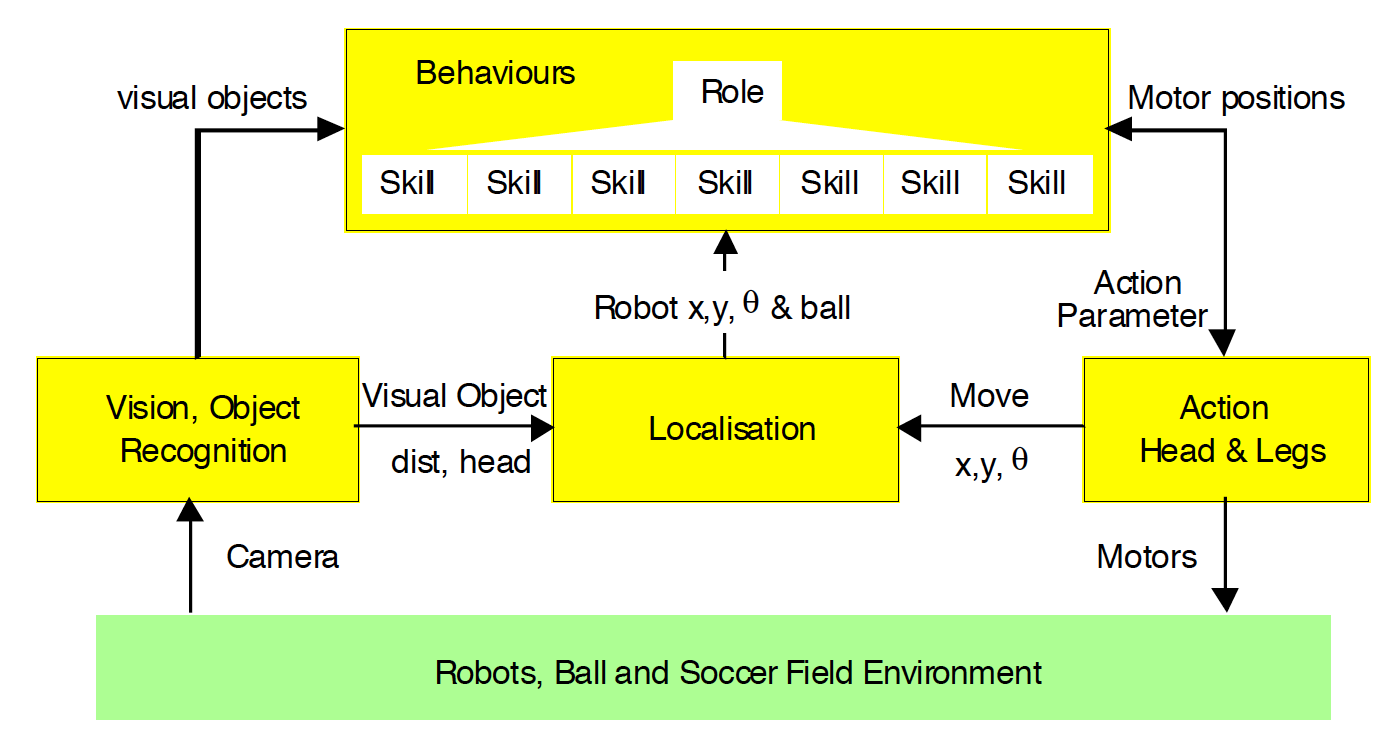
\includegraphics[width=0.7\textwidth]{figures/RoboticArchitecture2000}
\caption{The UNSW SPL robotic architecture used in the 2000 competition.} \label{figRoboticArchitecture2000}
\end{figure}

The robotic architecture used by rUNSWift was introduced in its basic form (\autoref{figRoboticArchitecture2000}) for the 2000 competition \cite{hengst00unswunited}, and while it has been developed in scope and to keep pace with new hardware platforms, it has remained essentially in tact.  Since 2000, wireless communication between robots has been added, and the robots, after being migrated through various versions of the Sony AIBO quadruped, have been replaced by Aldebaran's Nao biped. We discuss the 2010 robotic architecture in \autoref{sectionRoboticArchitecture2010} after briefly reviewing intelligent agents and agent architectures in general.  
 
\section{Agents and Agent Architectures}

Some communities are interested in agents as an advanced approach to software development. Our interests are in using agents as entities that implement artificial intelligence --- goal-directed sense-act systems. More specifically, we are interested in intelligent robotic systems embodying intelligent agents in situated physical systems that interact in real-time with real environments. 

Classical agent architectures rest on symbol manipulation systems. They are usually deliberative --- containing an explicitly represented symbolic model of the world in which decisions (e.g. actions) are made based on logical reasoning using pattern matching and symbolic manipulation \cite{Wooldridge95intelligentagents:}. An early symbolic agent architecture was STRIPS \cite{fikes71strips}, based on pre and post conditions that characterise actions, this system uses simple means-end analysis to try to achieve goals. 

Deliberative systems face two challenges that are hard to meet: how to translate the real-world  into an accurate symbolic description in time to be useful, and how to get the agents to reason with this description in time for the result to be useful. Despite much effort devoted to solve these problems, these architectures have difficulty in real-time control applications. 

Problems associated with symbolic AI led researchers to propose alternative approaches. Rodney Brooks for example proposed a \emph{subsumption architecture}, a hierarchy of behaviours competing with each other, with lower level behaviours having precedence over higher levels \cite{brooks86robot}. Brooks argued that the world is its own best model and the even simple rules could generate complex behaviour when interacting with a complex world.   

Reactive and deliberative systems are extremes on a spectrum of architectures. It seems reasonable to try to combine these approaches into hybrid robotic architectures to benefit from the advantages of each. This led to various \emph{layered} architectures, where the lowest layers provide a reactive circuit between sensors and actuators and higher layers deal with increasingly more abstract information, planning and reasoning on a longer time-frame.  Humans are a good example of hybrid architectures. We react quickly via our reflexes when touching a hot plate. The information is sent to the main part of the brain only \textbf{after} the action is carried out. On the other hand we also deliberate, often taking weeks to decide on our next holiday before we fly out. 

\begin{figure}[ht]
\centering
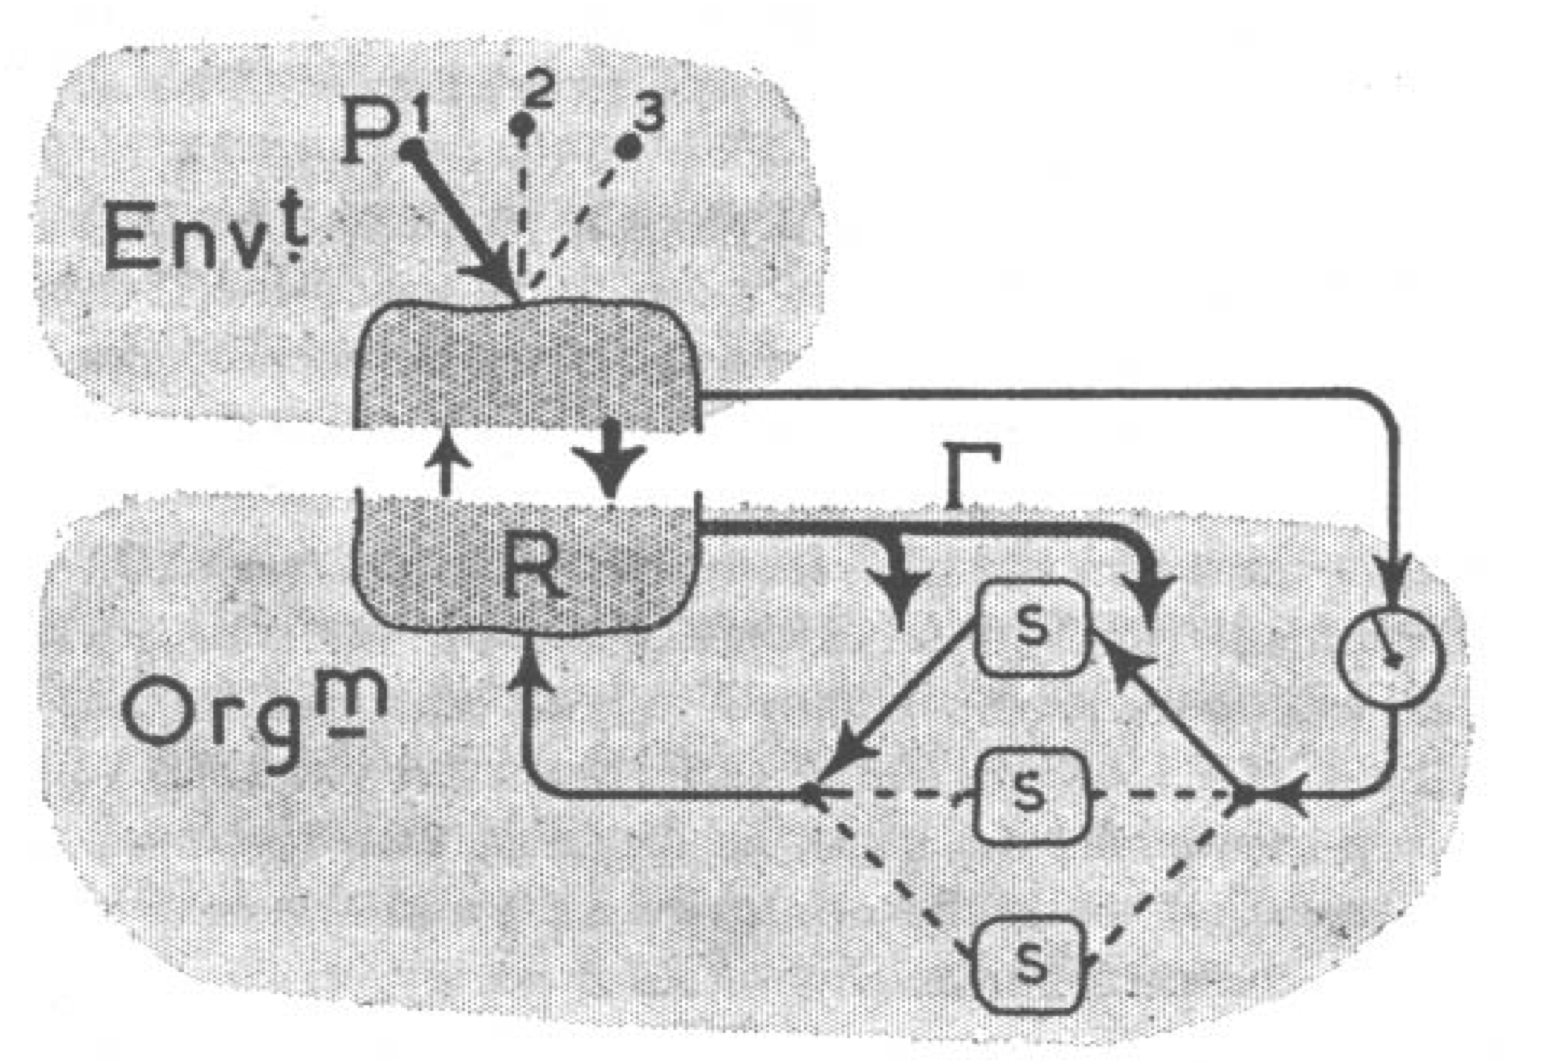
\includegraphics[width=0.4\textwidth]{figures/AshbyGating52}
\caption{Ashby's 1952 depiction of a hierarchically layered gating mechanism for more complex controllers, or regulators as he called them \cite{ashby52design}.} \label{figAshbyGating52}
\end{figure}

The idea of organising complex controllers in layered hierarchies has a long history. 
Ashby \cite{ashby52design} proposed a hierarchical gating mechanism (see
\autoref{figAshbyGating52}) for an agent to handle recurrent
situations. Behaviours are switched in by
``essential" variables ``working intermittently at a much slower
order of speed". Ashby commented that there is no reason
that the gating mechanism should stop at two levels and that the
principle could be extended to any number of levels of control.

A basic generic hybrid robotic architecture is the so-called three-layer (or level) architecture \cite{Gat97onthree-layer}. It consists of three components:
\begin{itemize}
\item A lower-level reactive feedback mechanism (Controller) with tightly coupled sensors and actuators with very little internal state.
\item A middle-level (Sequencer) that relies extensively on internal state  to sequence control at the lower-level, but does not perform any search.
\item A higher-level (Deliberator) that performs time-consuming (relative to relevant environmental dynamics) search, such as planning. 
\end{itemize}

An early example of a three-level architecture was ``Shakey the Robot" \cite{nilsson84shakey}. At the lowest level reflex stop actions are handled when touch-sensors detect an object and servo-control motors target their set-points. The intermediate level combine low-level actions depending on the situation. Plans are generated at the third-level. An example of a hybrid robotic architecture that learns how to respond to its environment is Ryan's RL-TOPs \cite{ryan00using} that combines planning at the top level and reinforcement learning at lower levels. 

\begin{figure}[ht]
\centering
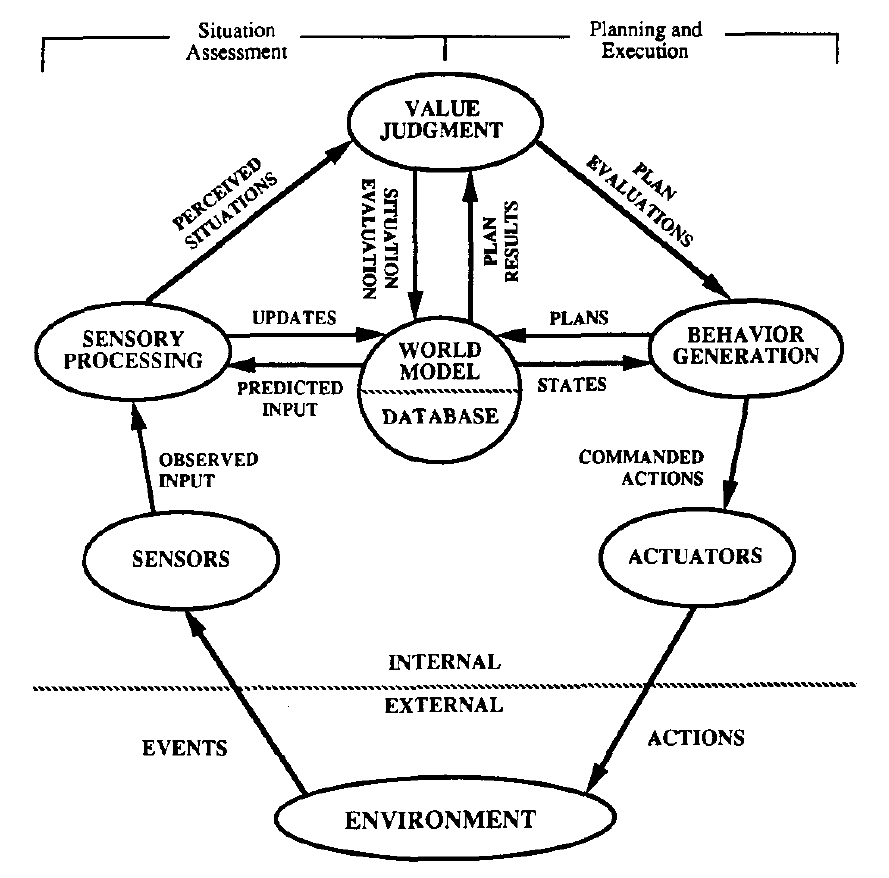
\includegraphics[width=0.6\textwidth]{figures/AlbusRoboticArchitecture91}
\caption{Albus's elements of intelligence and functional relationships forming the basis of a triple tower architecture.} \label{figAlbusRoboticArchitecture91}
\end{figure}

A generalisation of the three-level architecture proposed by Albus \cite{albus91outline} is the  triple tower architecture whose functional elements and information flows are based on modules flow as shown in Figure \ref{figAlbusRoboticArchitecture91}. This architecture is based on the Real-time Control Systems (RCS) that had been implemented at the National Institute of Standards and Technology (NIST). Albus's architecture was adapted and instantiated in a novel way by Nils Nilsson \cite{nilsson94teleoreactive}. 

\begin{figure}[ht]
\centering
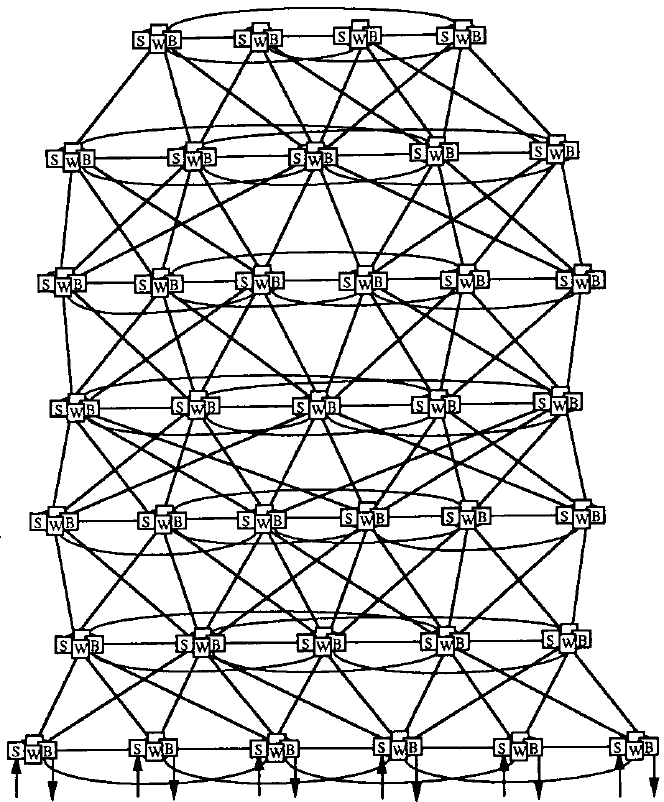
\includegraphics[width=0.4\textwidth]{figures/AlbusTaskHierarchy91}
\caption{Albus's real-time hierarchical control system consisting of modules of \emph{Sensor Processing(S)}, \emph{World-Modelling(W)}, \emph{Behaviour Generation(B), and \emph{Value Judgement} units.}} \label{figAlbusTaskHierarchy91}
\end{figure}

The three towers in the Albus's real-time control architecture relate to \emph{Sensor Processing(S)}, \emph{World-Modelling(W)}, and \emph{Behaviour Generation(B)} arranged in a (task) hierarchy -- \autoref{figAlbusTaskHierarchy91} -- in the form of a task-lattice. The rUNSWift robotic architecture can best be envisioned as instantiating a multi-robot task hierarchy to be elaborated in the next sections. 

The foregoing discussion on agent and robotic architectures is by no means comprehensive. Agent architectures in the literature abound. We will simply list a small subset of other agent architectures here with a short description:
\begin{description}
\item[ICARUS] is a computational theory of the cognitive architecture that incorporates ideas including work on production systems, hierarchical task networks, and logic programming \cite{langley91icarus} .
\item[SOAR] is symbolic cognitive architecture based on a symbolic production system \cite{Lehman96agentle}. A key element of SOAR is a \emph{chunking} mechanism that transforms a course of action into a new rule  
\item[BDI] stands for \emph{Belief-Desire-Intention} and is a software model for programming intelligent agents and has led to several agent implementations \cite{Rao95bdi}. 
\item[ACT-R] (Adaptive Control of Thought -- Rational) is a cognitive architecture that aims to define the basic and irreducible cognitive and perceptual operations that enable the human mind \cite{Anderson05humansymbol}.
\end{description}

\subsection{Task Hierarchies}\label{sectionTaskHierarchy}
The robotic architecture for rUNSWift is motivated by the formalisation of \emph{task-hierarchies} represented as \emph{task-graphs} \cite{Dietterich98hierarchicalreinforcement} that describe hierarchies of finite state machines \cite{hartmanis66algebraic}. These hierarchies are similar to the task-lattices of Albus in \autoref{figAlbusTaskHierarchy91}. Tasks are components (subtasks or sub-agents) of the architecture that accept input, perform a computation that can change the state of the component and produce output as a function of the input and component state. The output may be input to another component or invoke an action. When an action instantiates and executes another component it is an \emph{abstract} or \emph{temporally extended} action. When it has a direct effect on the agent's environment it is called a \emph{primitive} action. When subtasks terminate they \emph{exit} and return control to their parent task. The states of the parent subtask represent the blocks of a partition of lower-level states and we refer to them as \emph{abstract} states.  

\begin{figure}[ht]
\centering
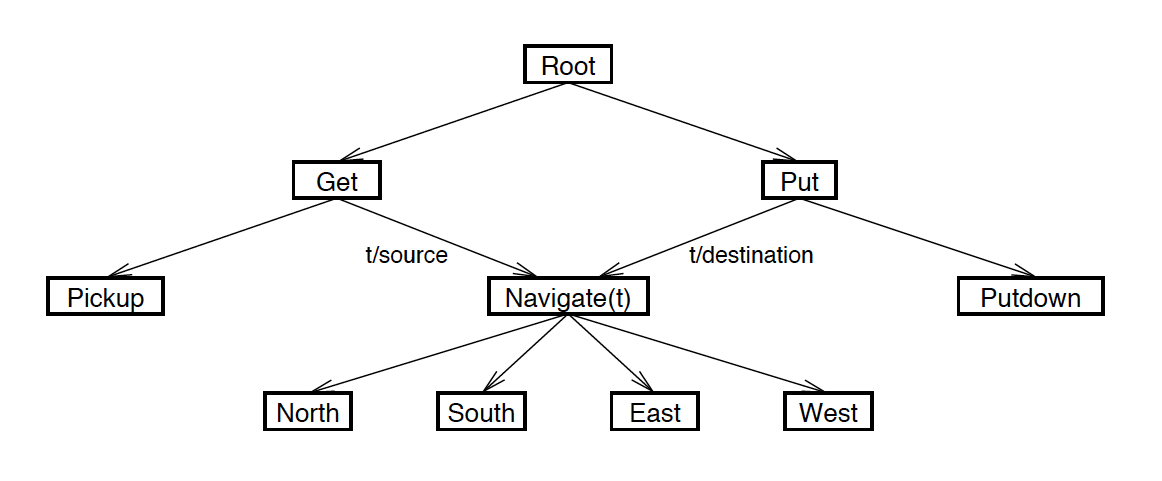
\includegraphics[width=0.5\textwidth]{figures/TaxiTask}
\caption{The taxi task-hierarchy task-graph in  \cite{Dietterich98hierarchicalreinforcement}.} \label{figTaxiTask}
\end{figure}

An illustration of a task-hierarchy is Dieterich's taxi task shown in \autoref{figTaxiTask}. This task-hierarchy has been devised for a grid-world taxi that can move in four compass directions with the aim of picking up, transporting and putting down passengers. The sub-tasks consist of primitive actions for moving, loading and unloading passengers, as well as temporally extended actions for pick-up, put-down and navigating. For example the subtask $Get$ has one abstract state that represents an empty taxi at any location. $Get$ invokes a child subtask $Navigate(t)$, where $t$ is a destination, and a $Pickup$ subtask. On exit of $Get$, $Root$ invokes subtask $Put$. 

Each sub-task module, invoked by a parent, senses the state it is in, and using a model of its effects and a value-function over states, takes actions (behaviour).  In this way complex behaviour responses can be succinctly encoded at various levels of abstraction and skills reused. 

\section{rUNSWift 2010 Robotic Architecture} \label{sectionRoboticArchitecture2010}

The rUNSWift robotic architecture is a task-hierarchy for the multi-agent team of three Naos. As there is no central controller this architecture is implement on each robot. This means that each robot may have a slightly different view of the world and therefore its role on the team. This restriction is imposed by the event organisers, but has the advantage of providing some redundancy in case individual robots are disqualified or stop working.

Starting at the root-level the game-controller invokes the high-level states for playing soccer (see \autoref{sectionrUNSWiftExecutable}). At lower levels, the walk generators execute temporally extended walk phases (e.g. \autoref{sectionSlowWalk} \autoref{sectionFastwalk}) that invoke primitive state transitions constituting the motion of the robot as it transitions between poses 100 times each second. The omni-directional walk and kick generators are themselves task-hierarchies (see for example \autoref{figFastwalkTaskgraph} in \autoref{sectionFastwalkTaskHierarchy}) with the effect that the total rUNSWift robotic architectures may execute through a nine-level task-graph in some instances.  

\begin{figure}[!htp]
\centering
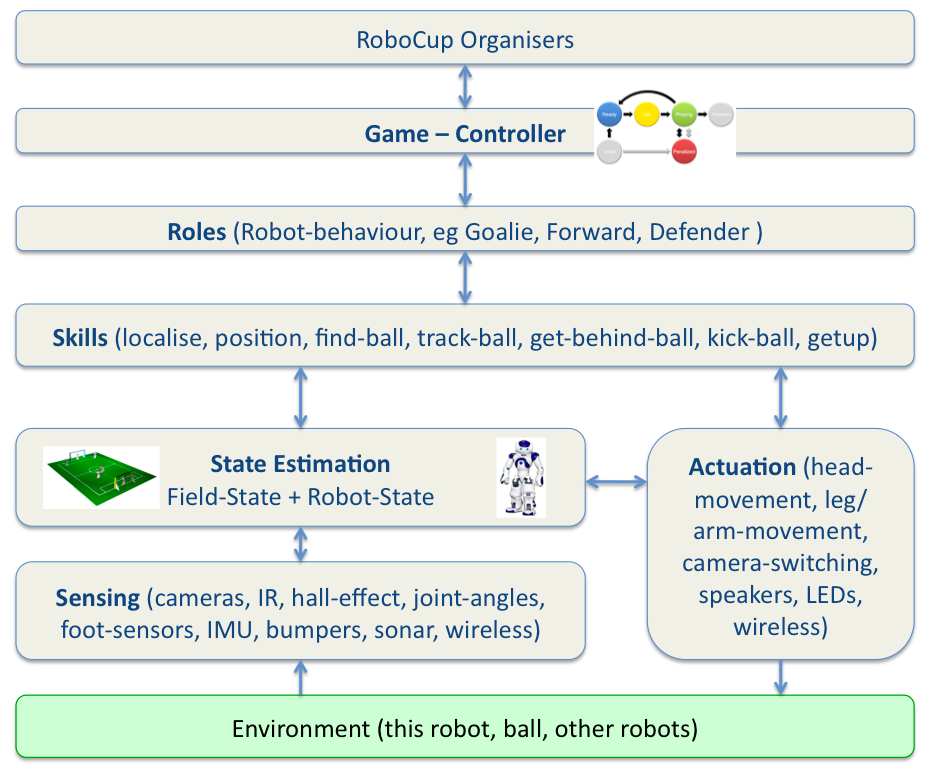
\includegraphics[width=0.6\textwidth]{figures/runswift2010architecture}
\caption{The 2010 UNSW SPL robotic architecture.} \label{figrunswift2010architecture}
\end{figure}

\emph{State Estimation} in \autoref{figrunswift2010architecture} consists of the \emph{field-state} and the \emph{robot-state}. The field-state refers to the relevant environmental characterisation the includes the position and orientation of all the robots (our own and those of the opposition) plus the location and motion of the ball. The robot-state are estimates of variables that characterise the environment consisting of the internal state of the robot that determines its dynamical properties such as position of joint angels, velocity, acceleration, and center-of-mass. While this distinction is largely arbitrary, the dichotomy into field and robot state is to separate their different purposes. The field-state is used for determining strategy and behaviour, whereas the robot state is used for the control of motion at lower-levels in the task hierarchy.

State estimation is akin to the world-model in \autoref{figAlbusRoboticArchitecture91}. State variables are estimated using Bayesian filtering techniques with observations from sensors. A large part of the computational effort is expended in preprocessing relevant visual features in the environment (\autoref{sectionVision}) and localising the robot using both Kalman and Particle filters (\autoref{sectionLocalisation}). 

\emph{Actuation} refers to the movement of the head, body, arms and legs to effect walking, kicking and getup routines. This is describe in \autoref{sectionMotion}. It  also includes other actuators such as audio speakers, LEDs and wireless transmission. The higher levels of the task-hierarchy for skills and behaviours are described in \autoref{sectionBehaviour}.

\begin{figure}[!htp]
\centering
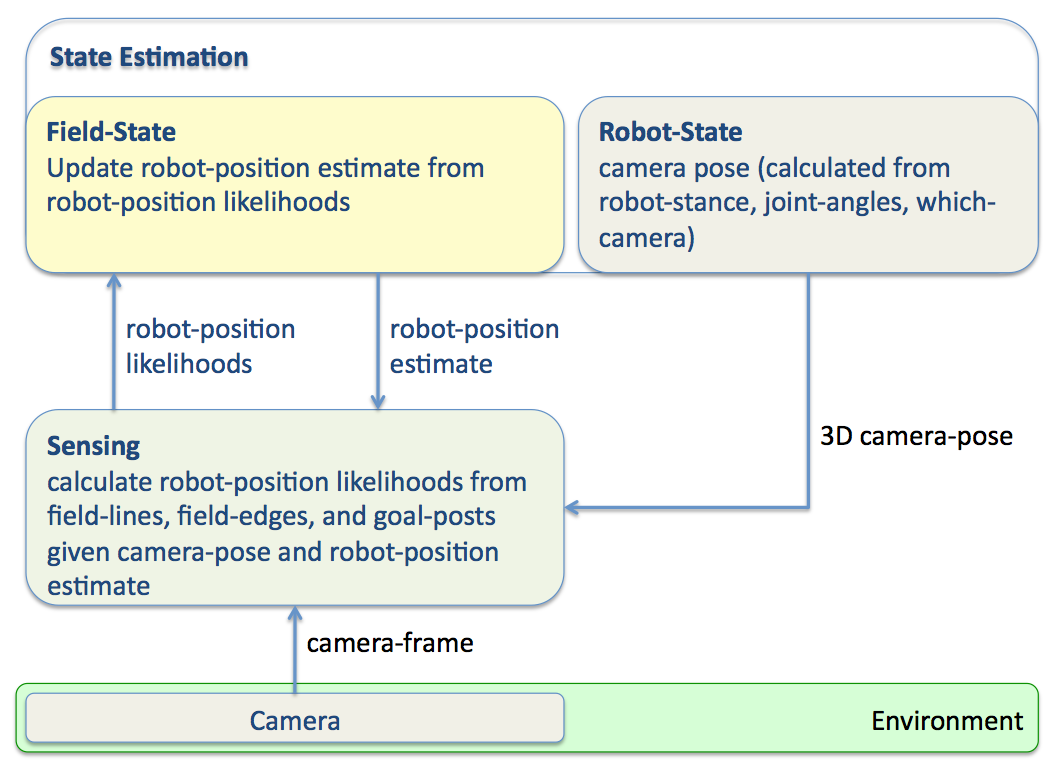
\includegraphics[width=0.5\textwidth]{figures/FieldState}
\caption{The FieldState.} \label{figFieldState}
\end{figure}

\autoref{figFieldState} shows details on how the field-state is updated. Visual sensing is performed in the context of the robot state (e.g. where it is looking) and the current estimate of the filed state. For example, the stance of the robot allows the determination of a horizon the in turn places constraints on the position of objects --- we would not expect to see the green field above the horizon. Equally, the estimated position of the robot on the field can provide constraints (context) for the vision system. This is discussed further in \autoref{sectionVision}. 

\begin{figure}[!htp]
\centering
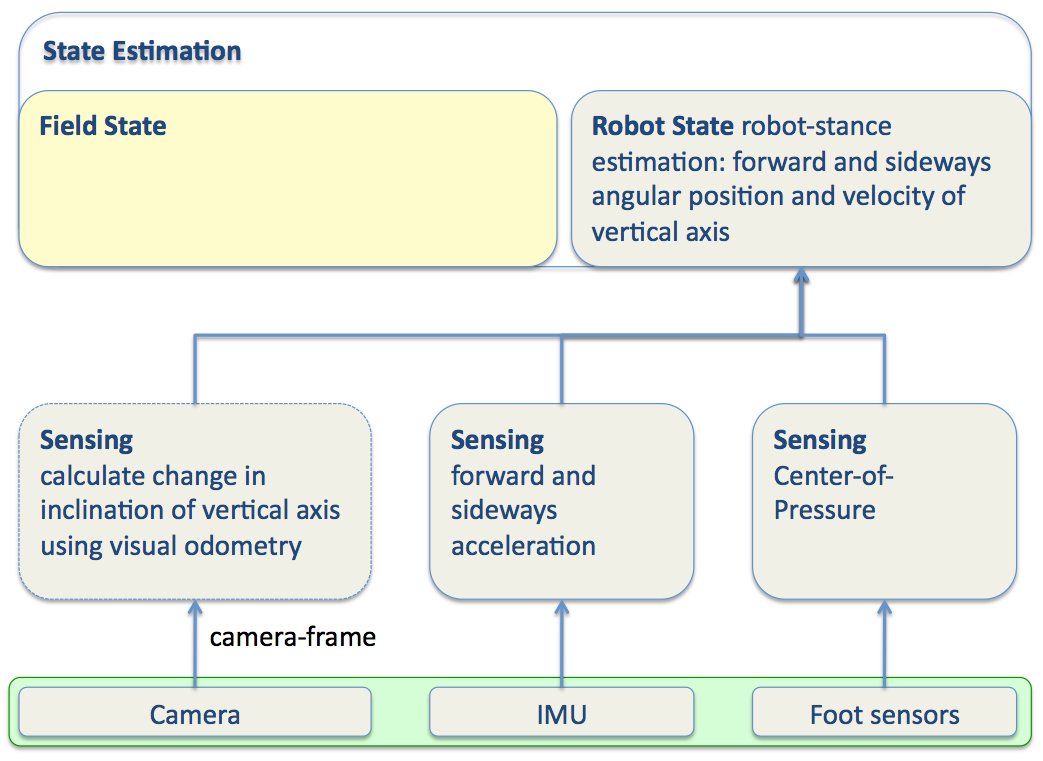
\includegraphics[width=0.5\textwidth]{figures/RobotState}
\caption{The RobotState.} \label{figRobotState}
\end{figure}

\autoref{figRobotState} shows the sources of observational information to estimate the robot state. They are foot-sensors for both the sagittal and coronal center-of-pressure, the inertial-measurement-unit (IMU) located in the Nao's chest providing linear and angular accelerations, and optic-flow via the cameras. The later has not been implemented this year.

\section{Conclusions and Future Work}
The rUNSWift robotic architecture has stood the test of time and is consistent with several other architectures that have been developed for real-time control. We have two aspirations for future developments and use of this architecture. We plan to formalise the operation of the task-hierarchies including multi-tasking (partially ordered) and concurrent (simultaneous) actions. Secondly, we plan to learn the task hierarchies using various techniques such as reinforcement learning \cite{sutton98reinforcement}, structured induction \cite{shapiro87structured}, and behavioural cloning \cite{Bain96aframework}. 

% **********************************************************************************************************
\newpage
\chapter{System Implementation}

\section{Interacting with the Nao robot}

The Aldebaran Nao robot is provided with a fully-functional Linux operating
system, as well as custom software from Aldebaran called \emph{NaoQi}, which
allows interaction with the hardware. The \emph{Device Communications Manager}
module of NaoQi is the only practical way to actuate the joints and LEDs of
the robot and read sensors, including joint angle sensors, accelerometers,
and sonars.

rUNSWift of previous years have used \emph{ALProxy} to communicate with NaoQi.  This
allowed us to have our code as either a library or a standalone executable. 
When our module was embedded as a NaoQi library, ALProxy would communicate
directly with NaoQi via a C++-like API.  When run separately, ALProxy would use
a slow, TCP-based protocol.

It is standard practise to program the robot by producing a dynamic library
that is loaded by NaoQi when the robot boots, this allows for close
interaction between third party code, and the NaoQi DCM module. The
disadvantage of this approach is the added difficulty in debugging, and
recovery from crashes. To avoid damage to the robot, and to isolate
potentially dangerous and complex code in the robot's control system from
low-level hardware interaction, we have developed two separate binary
packages that we deploy to the robot: \emph{libagent} and \emph{runswift}, which
communicate using a block of shared memory and a semaphore. They are
described in the following sections.

\subsection{The `libagent' NaoQi module}

The primary purpose of libagent is to provide an abstraction layer over
the DCM that has the simple task of reading sensors and writing actuation
requests. Due to its simplicity, is is less likely to contain errors, and
thus less likely to crash and cause the robot to fall in a harmful way.

The DCM provides two functions, \texttt{atPreProcess} and
\texttt{atPostProcess}, to register callback functions which are called before
and after the 10ms DCM cycle, respectively. In the pre-DCM-cycle callback
function, we read the desired joint and LED commands from the memory shared with
`runswift', and use the DCM's \texttt{setAlias} commands to actuate the robot.
In the post-DCM-cycle callback function, all sensor values are read into shared
memory.

In order to use the Aldebaran omni-directional walk, libagent was expanded
to abstract the ALMotion interface as well, allowing us to use the walk
from runswift. We did this by having a special flag in our joint angles
array that specified whether it was to be read as a joint command or an
Aldebaran walk command. If this flag is enabled, the array was to be filled
with the Aldebaran walk parameters \emph{x}, \emph{y}, \emph{theta},
\emph{frequency} and \emph{height}, instead of joint angles. These values
are passed to ALMotion, using the \emph{setWalkTargetVelocity} command.

There is also a flag to indicate that the walk should stop. When this flag
is received by libagent, it stops passing the commands on to ALMotion, and
instead transitions to a standing pose using the
\emph{post.angleInterpolation} command. This provides a fast transition out
of the Aldebaran walk. Previously, before the transition, the legs were
brought together by making an infinitesimal step with the \texttt{walkTo}
command. However, this is a lot slower and the current interpolation-only
method is only marginally more unstable.

To facilitate in-game debugging, without the need to connect an external
computer to the robot, a  variety of features were added to libagent. These
included a system of button-presses to perform various actions, such as
releasing stiffness or running system commands. Most system commands are
run using the C \texttt{system} call, however some commands need to
shut-down NaoQi (such as to flash some of the robot's control boards).
These cannot be run in the usual manner, as they will be children of NaoQi
and will be killed when NaoQi is killed. For these, we call scripts using
custom run-once init levels, which have init as a parent (\autoref{fig:runlevels}).

\begin{figure}
\begin{center}
   \begin{minipage}[h]{0.6\textwidth}
      \begin{verbatim}
nr:a:once:/etc/init.d/naoqi restart
fa:b:once:/home/nao/bin/flash-all
fc:c:once:/home/nao/bin/flash-chestboard-wrapper \end{verbatim}
   \end{minipage}
   \caption{The changes made to \textbf{/etc/inittab} to create custom run-levels.}
   \label{fig:runlevels}
\end{center}
\end{figure}

The libagent module will also take over the use of the LEDs for debugging
purposes. The ear LEDs are used to indicate battery level, with each lit
segment indicating $10\%$ capacity. Additionally, if libagent is
controlling the robot's motion (for instance, if the user has manually made
the robot limp, or runswift has lost contact with libagent), the chest LED
is overrode to display this information. If just the head is made limp by
the user, the top segment of the eye LEDs are overridden.

In the event that the runswift executable crashes or freezes, it will stop
reading sensor values from libagent. If it misses a certain number of
libagent cycles, libagent will assume it is no longer running and initiate
a ``safety stop''. This is a slow transition to a stable position where the
robot is crouching down supported by both its legs and its arms. This was
not needed in the competition, but was quite useful during development.

The libagent module also monitors the temperatures of the joints, and if
they exceed 70 \textdegree C, will use speech to vocally warn the user that
the joints are approaching the upper limit of their functioning (the
current flowing to the joint starts to be limited from 75 \textdegree C
\cite{aldebaran10developer}). This was quite useful, as the FastWalk is
quite intensive and can quickly wear robots out.  With the warning, we were
able to switch to other robots and avoid wearing robots out completely.

\subsection{The `runswift' Executable}\label{sectionrUNSWiftExecutable}

\emph{runswift} is a stand-alone linux executable, detached from NaoQi for safety and debugging. It uses \emph{Video4Linux} to read frames from the Nao's two cameras, reads and writes to a shared memory block, synchronised with libagent, to read sensor values and write actuation commands, and performs all the necessary processing to have the Nao robot play soccer.

Because it is detached from NaoQi, it is easy to run runswift off-line, with the Motion thread disabled, allowing for vision processing and other testing to take place without physical access to a robot. It can be run using any of the standard linux debugging wrapper programs including gdb and valgrind, which are invaluable when resolving memory-related issues.

The \emph{runswift} executable is a multi-threaded processing, featuring 6 threads: Perception, Motion, Off-Nao Transmitter, Nao Transmitter, Nao Receiver and GameController Receiver. All of these except for Perception are IO bound, providing reasonable multithreading performance on a uniprocessor, such as the AMD Geode found in the Nao.

The Perception thread is responsible for processing images, localising, and deciding actions using the behaviour module. The Motion thread is a real-time thread, synchronised with libagent, and therefore the DCM, that computes appropriate joint values using the current action command and sensor values.

The other threads are all networking related, and with the exception of GameControllerReceiver, use the Boost::Asio C++ library to provide a clean abstraction over low-level TCP/IP sockets.

% This is duplicated later on??
% The Boost::program\_options library is used to parse configuration files and command-line arguments, giving a high degree to flexibility to the way the `runswift' executable is used. Everything from player number and team number, through debugging options such as log level, to parameters for walks, can be set using the program\_options. The options are read in a hierarchical fashion: First \emph{runswift.cfg} is read, which contains parameters that apply to the entire team of robots, such as network configuration and game type. Second \emph{hostname.cfg}, where hostname corresponds to the particular robot in use, is read, this contains information such as the player number. Finally, options entered on the command line are read, this method is usually reserved for testing and debugging, and is not used in-game.

A key feature of the \emph{runswift} executable is the \emph{ThreadWatcher}. Each of runswift's threads are started using \emph{pthread\_create()}, with the starting point set to a templated \texttt{SafelyRun} function, that wraps a thread in a number of safety features:\begin{itemize}
\item{A timer, that audibly alerts the user if a thread's cycle takes longer than its expected maximum runtime}
\item{A generic exception handler, that will log unhandled exceptions and restart the failing module}
\item{A signal handler, that will catch unhandled SIGSEGV and SIGFPE signals, indicating an error in the module. These errors are logged before the module is reconstructed, leaking memory but continuing to function.}
\end{itemize}
All of these safety features have saved us from having to request a robot for pickup during games, which would have resulted in a 30 second penalty under the SPL rules.

\section{Debugging}
Debugging software running on a robotic platform adds additional challenges compared with traditional software. Problems are often difficult or impossible to reproduce due to the inability to re-create the precise circumstances where the fault occurred. Noisy sensors make it impossible to re-enter precisely the same inputs to a system multiple times. To help in the creation of robust robotic software, we have developed several techniques for debugging, described in the following sections.
\subsection{Logging}
The simplest means of debugging is dumping the current state of some part of the
robot's memory to disk. We have developed a C++-stream style logging utility
called `llog'. llog writes to a log file with the same name as the current
source directory, separating the log files on a per-module basis automatically.
It also supports several log levels, modeled after ssh\cite{sshconfig}:
DEBUG\{321\}, VERBOSE, INFO, WARNING, ERROR, QUIET and SILENT. Rather than
setting the log level as a compile-time option, it can be chosen at runtime with
a simple run-time option, saving the need to recompile whenever additional
output is needed.

llog avoids making a system call for llog calls below the current log level by
returning a \emph{null stream} that discards its input, and overloads all the
necessary operators to function correctly as a stream. To further reduce the
overhead of logging, all logs are written to volatile memory on the Nao, to
avoid large performance differences caused when data has to be synced to disk.
Log files can be recovered from the Nao over the network before the Nao is
switched off.
\subsection{Off-Nao}
The rUNSWift Nao teams of previous years used, to the best of their ability,
the OffVision tool, written by the rUNSWift AIBO teams.  This tool was written
with the Qt3 widget toolkit, and it was apparent that the knowledge of the inner workings of the tool faded away over the years.

Off-Nao is a new desktop application written with the Qt4 widget toolkit, which
streams data from the Nao using a TCP/IP connection established using the
boost::asio C++ library. Recordings can be reviewed in Off-Nao, to help
determine the relationship between a sequence of observations and the resulting
localisation status determined on-board the robot, as well as other
correlations not determinable in real-time.

Off-Nao can also separately run the runswift vision module on a sequence of recorded frames, allowing for reproduction of errors and regression testing of vision enhancements.

The following is a brief overview of each debugging module currently present in Off-Nao.

\begin{description}
\item[Overview Tab] As depicted in \autoref{figOverviewTab} the Overview Tab
has three primary methods of visualising information streamed from the Nao. 

First, if available the saliency scan or raw image will be displayed in the top right display box. Overlays of objects detected through vision are then rendered on top of this image.

Second, the absolute positions of objects the Nao perceives are displayed on a
2D field. This is useful for debugging localisation as any anomalies may be
quickly recognised when it is rendered on a 2D field such as this.

Lastly, a data list is available for displaying raw data so that values such as the frame rate and the exact values of the data rendered in the previous two methods may be known.

\begin{figure}[ht]
\centering
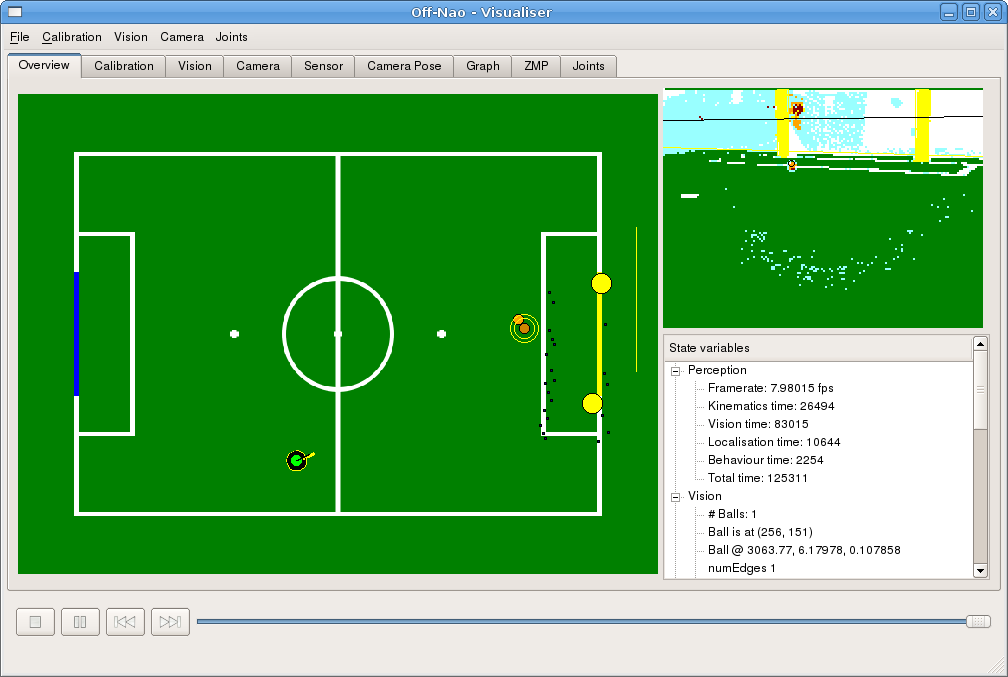
\includegraphics[width=1.0\textwidth]{figures/overviewTab}
\caption{Overview tab.} \label{figOverviewTab}
\end{figure}


\item[Calibration Tab]
As described in \autoref{sec:camcolcalib}, our vision system requires the manual generation of a colour lookup table, mapping YUV triples to one of 8 colours found in the standard SPL environment. This tab, shown in \autoref{figCalibrationTab} allows a team member to carry out this process. Raw images can be overlayed with all SPL colours, or just one currently being trained. Furthermore, the vision module can be run on the image under scrutiny, to test if the changes made to the colour calibration affect feature detection. This tab can also display a point cloud, shown in \autoref{figPointCloud}, that visualises the locality of SPL colours in YUV space. This allows the team member to view the effects of their changes to the calibration, and identify pairs of colours that border one another closely, and therefore might need more fine-grained classification.

\begin{figure}[ht]
\centering
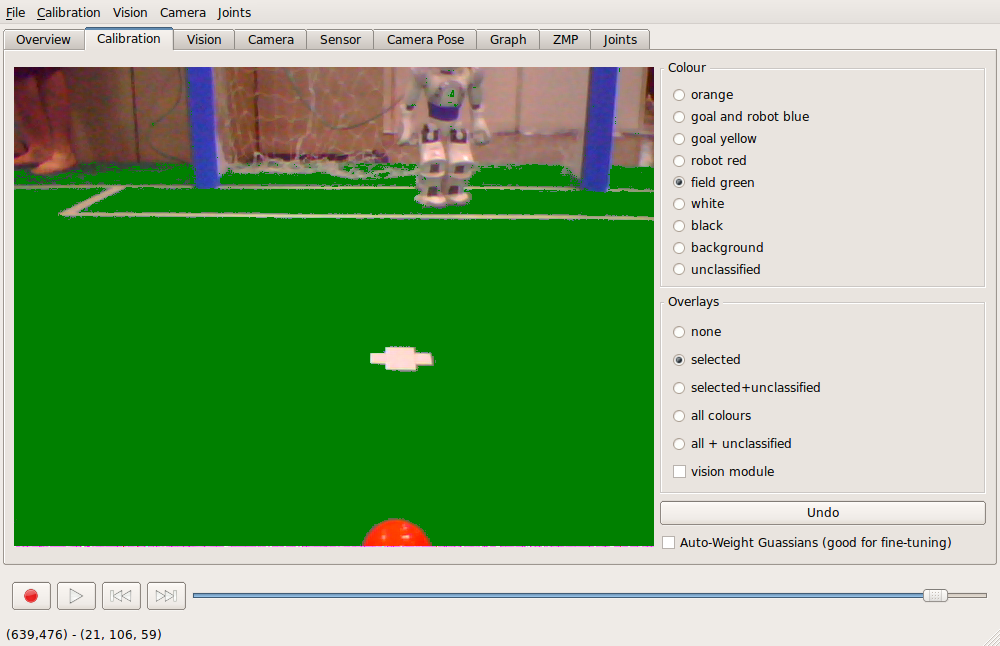
\includegraphics[width=1.0\textwidth]{figures/calibrationTab}
\caption{The Off-Nao calibration tab, used to generate colour look-up tables.} \label{figCalibrationTab}
\end{figure}

\begin{figure}[ht]
\centering
\centering
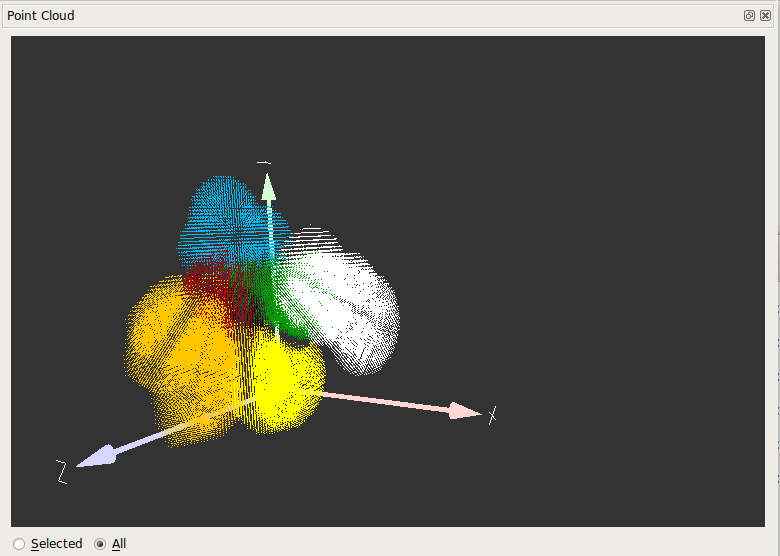
\includegraphics[width=0.7\textwidth]{figures/pointCloud}
\caption{A visualisation of the colour calibration in YUV space, launched from the Off-Nao calibration tab.} \label{figPointCloud}
\end{figure}

\item[Vision Tab]
The vision tab as seen in \autoref{figVisionTab}, is used to visualise
object detection on either; frames streamed live over the network or dump
files previously saved from the robot. Similar functionality is available
on the Calibration tab however this tab allows for the ability to selectively choose which object detection overlays are to be displayed.
\begin{figure}[ht]
\centering
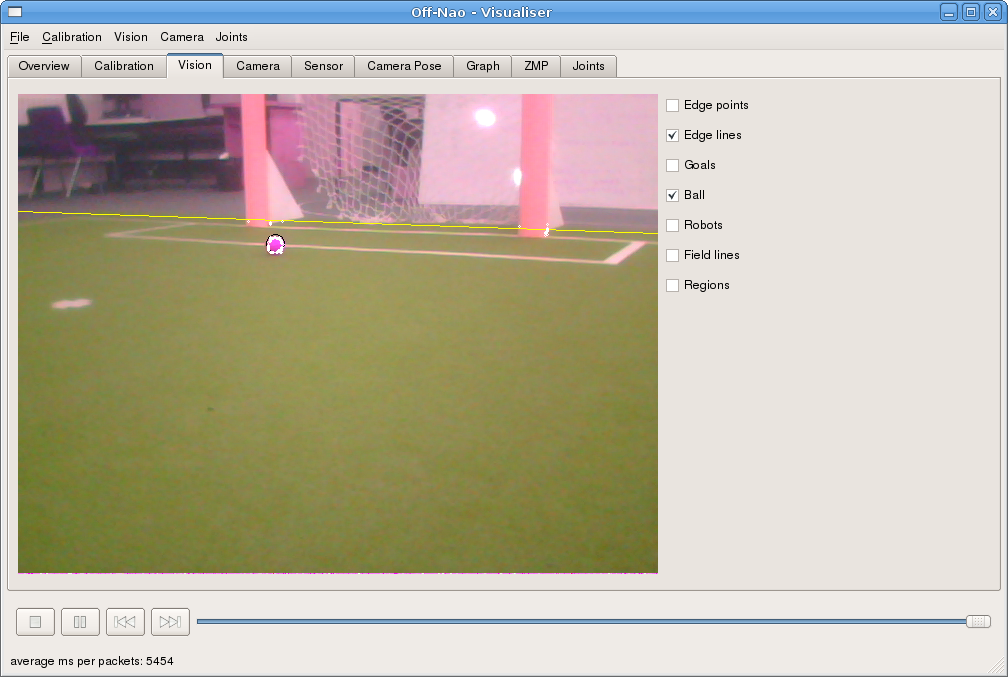
\includegraphics[width=1.0\textwidth]{figures/visionTab}
\caption{Vision Tab} \label{figVisionTab}
\end{figure}



\item[Graph Tab]
The Graph Tab, as depicted in \autoref{figGraphTab}, is used to graph
the Accelerometers, Foot Sensors, Torso Tilt, Sonar, Battery Charge and Battery Current. This has the primarily purpose of assisting in the development of walks and to help interpret sensor data.


\begin{figure}[ht]
\centering
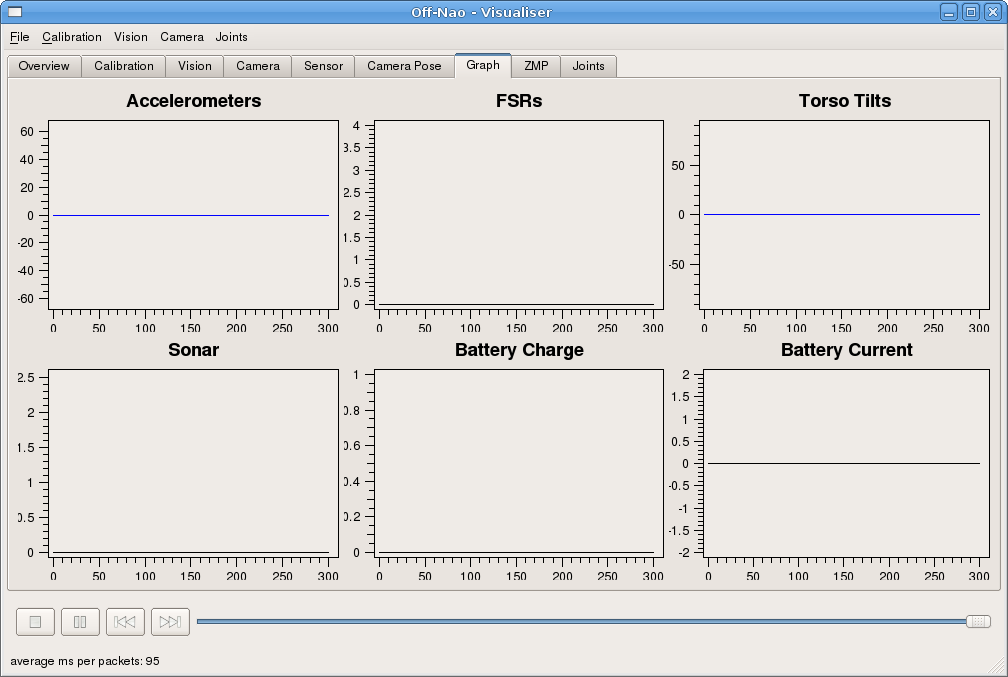
\includegraphics[width=1.0\textwidth]{figures/graphTab}
\caption{Graph Tab} \label{figGraphTab}
\end{figure}

\item[Kinematic Calibration Tab]
As depicted in \autoref{figKinematicsCalibration}, this tab is used to
calibrate the Kinematic chain for the Nao robot. The process used to do this is
further described in \autoref{kinematicCalibration}.

\begin{figure}[ht]
\centering
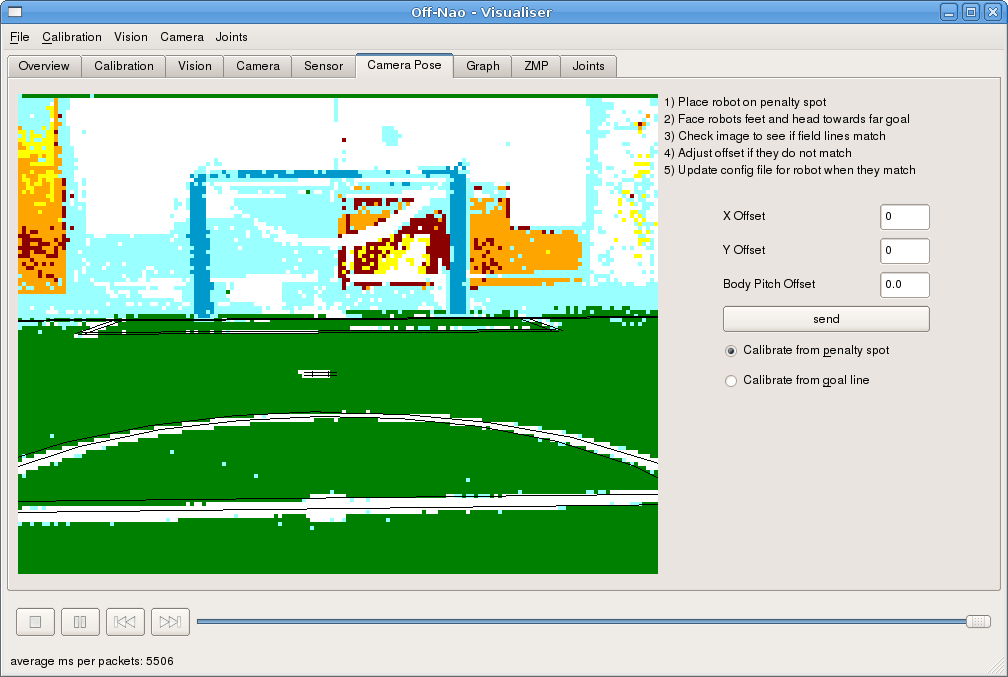
\includegraphics[width=1.0\textwidth]{figures/kinematicsCalibration}
\caption{Kinematic Calibration Tab.} \label{figKinematicsCalibration}
\end{figure}



\end{description}

\subsection{Speech}
In SPL games, no network interaction between the team of human programmers
and the robot is allowed, so the Nao vocalises any serious issues that
occur using the \texttt{flite} speech library. The robot informs us when
its key systems start and stop, and of any unhandled exceptions caught or
crashes detected. This can be invaluable during the game, as it allows us
to quickly identify problems such as the network card falling out or the
sonars malfunctioning, so that the team captain can quickly call for a
`Request for Pickup' to restart the robot or some of its software through
the button interface.

The calls made to \texttt{flite} are non-blocking. This is for two reasons:
\begin{itemize}
    \item It allows us to use speech debugging from real-time threads,
        \textit{e.g.} the DCM callbacks.
    \item It allows us to say things as close to when they actually
        happened as possible, instead of later speech events being delayed
        by earlier ones.
\end{itemize}
To implement this, we have a \emph{SAY} function that forks a new,
low-priority thread (this prevents speech debugging from inheriting the
real-time scheduling of the Motion code). This thread then calls
\texttt{flite} with the text to speak as an argument. This has the added
benefit that we don't need to maintain a thread-safe queue, since every
\emph{SAY} call forks a new thread.

\section{Python interpreter}
\subsection{Automatic Reloading for Rapid Development}
To facilitate the rapid development of behaviours, we chose to use a dynamic language, Python. The Python interpreter was embedded into the \emph{runswift} C++ executable using libpython. The inotify library for Linux was used to monitor a directory on the robot containing Python code, and reload the interpreter whenever Python code changes.

The inotify library can be configured to monitor a directory using the following system calls:

\begin{lstlisting}
   int inotify_fd = inotify_init();
   int wd = inotify_add_watch(inotify_fd, "/home/nao/behaviours",
         IN_MODIFY|IN_ATTRIB|IN_MOVED_FROM|IN_MOVED_TO|IN_DELETE);
\end{lstlisting}

Each Perception cycle, a change can be detected by using a \texttt{select()} syscall on the inotify\_fd, followed by a \texttt{read()} into an inotify\_buffer if new data is available. The name of the event can be compared to the regular expression \texttt{.*$\backslash$.py} to check if it is a Python file that has changed, and if so we reload Python using the standard calls from libpython that re-initialise the interpreter and load our modules:

\begin{lstlisting}
   if (Py_IsInitialized()) {
      Py_Finalize();
   }
   Py_Initialize();
   /* Add a static module of C++ wrapper functions */
   initRobot()
   PyImport_ImportModule("ActionCommand")
   PyImport_ImportModule("Behaviour")
\end{lstlisting}

The static module \emph{Robot} provides Python behaviours with access to data from the other C++ modules in runswift. The Python behaviours are also required to return an ActionCommand to C++ through a callback function, setting the next desired action of the robot.

This architecture allows us to make small modifications to behaviour and upload them to the robot using \textbf{nao\_sync} whilst runswift is still running. The robot's motion thread is uninterrupted, so it will continue walking, standing or kicking as per the ActionCommand request on the Blackboard. When the replacement Python code is uploaded, the Perception thread continues with the behaviours reset.

In contrast, to do development with pure C++ behaviours, it is necessary to re-compile runswift, re-link runswift, upload the executable, stop the robot safely, then start it again with all systems re-initialised. It is clear that writing behaviours in a dynamic auto-reloadable language such as Python, provides great improvements to a team's productivity.

\section{Network Communication}

\subsection{GameController}

The runswift executable uses legacy code from the Aibo league to receive broadcast packets from the electronic referee. These are then acted upon at the Behaviour level.

\subsection{Inter-Robot Communication}

The \emph{boost::asio} C++ library is used to broadcast information from each robot at
5 Hz to each of its team-mates, informing them of its position and the position
of the ball, this information is incorporated at the Localisation level.

\begin{notesfornextyear}
\subsection{Off-Nao}

As mentioned earlier, Off-Nao also uses the boost::asio library to communicate
with runswift.  Off-Nao sends a bitmask of requested fields (blackboard,
saliency image, raw image, position particles) and runswift sends the requested
fields to the connected Off-Nao.  Each connected Off-Nao can use a different
bitmask.

Each field is sent as a binary copy of data, with special handling.  For the
blackboard, the blackboard members that are located in memory outside the
blackboard, such as an STL list, the member is serialised using
boost:serialization, then sent across.  For STL containers, before being
de-serialised, they are initialised to the empty container in a non-portable
fashion, as the boost de-serialisation operation empties the container before
de-serialisation.

For the saliency image, RLE is done to compress the sent data, and for the raw
image, a zlib compression operation is performed.  In both of these cases, a
lock is performed so that shearing of the image does not occur.
\end{notesfornextyear}

\subsection{Remote Control}

The remote control subsystem comprised two components. The first component 
consisted of a variety of changes to Off-Nao to accept controls from the 
keyboard and to send them over the channel to the robot. The commands needed 
to be continually sent to enable smooth robot movement, ensure the robot did 
not fall over, and make sure that the current behaviour was correctly 
overridden when remote control was enabled. The robot speed was calibrated to
increase gradually to enable accurate control.

These commands could be used anywhere in the Off-Nao system and were not 
restricted to a particular tab. On the robot side, the command was picked up
from the channel when the robot was connected to Off-Nao and sent one of these
remote-control overrides. This command would then be used in lieu of whichever
action-command had been determined from a behaviour. 

\section{Configuration files}

To allow the team to dynamically assign roles, kinematics offsets, and other per-robot variables without rebuilding \emph{{runswift}}, the boost::program\_options library was used. This allows options to be parsed in a hierarchical manner:

\begin{itemize}
   \item{Default values, specified in source code}
   \item{Values in `runswift.cfg'}
   \item{Values in `robotname.cfg'}
   \item{Values specified as command-line options}
\end{itemize}

As such, it was easy to set team-wide variables using `runswift.cfg', robot-specific details such as player number in `robotname.cfg', as well as overriding arbitrary values on the command line during development.

A typical robot's configuration file may looks like this:

\begin{lstlisting}
[player]
number=2
team=19
ip=107

[kinematics]
cameraoffsetXbottom=0.0
cameraoffsetYbottom=1.0
cameraoffsetXtop=0.4
cameraoffsetYtop=-2.9
bodyPitchOffset=2.5
\end{lstlisting}
% **********************************************************************************************************
\newpage
\chapter{Vision} \label{sectionVision}

\section{Introduction}

Automatic identification of objects in a video feed is a significant research area in robotics, and forms the major component of the robot's sensory perception of the world. While the structured area of a soccer field permits the use of algorithms tailored for the identification of specific objects, such as the orange balls used in the competition, a game of soccer played using the Nao robots presents specific and complex challenges in the field of computer vision, including: \begin{itemize}
\item{The vision processing system has to run fast enough to provide up-to-date information for other systems to process. This means frames should be able to be processed at 30 frames per second}
\item{It is required to run on the Nao's 500MHz processor}
\item{Objects must be identified accurately enough to allow kinematics to provide reasonable estimates of their distance away from the robot}
\item{It must be robust enough to perform with a high level of image blurring}
\item{It must identify false positives as little as possible}
\item{It must be robust enough to handle a significant amount of object occlusion}
\end{itemize}

Our overall approach to object identification relies heavily on both colour classification and edge detection. Colour classification allows fast identification of approximate areas of objects such as goals and balls, while edge detection allows the positions of these objects to be found very accurately in the image, and provides a substantial amount of robustness to uneven and changing lighting conditions. 

In order to make our object identification run as efficiently as possible, we start our processing on a frame by subsampling the frame to produce a 160 by 120 pixel colour classified image. From this saliency scan, we can quickly identify probable locations of the various objects we need to identify. The full resolution image can then be used to accurately determine the location of each of these objects in the frame. After the saliency scan is built, we identify the edge of the field in the image using the saliency scan, or that the entire frame is below the field edge. Using this information, the part of the image that contains the field is scanned to identify and grow regions that could possibly contain balls, robots or field lines. The shape and colours of the pixels in these regions is used to identify the most probable object they contain, and specific algorithms for ball, field line and robot detection can be used on the appropriate regions to reliably and accurately identify the objects. Goal detection is performed separately as the goal are mostly above the field edge; instead using histogram information generated with the saliency scan to approximately locate the goals. 

Once the position of an object in the image has been identified, we use a
kinematics chain to estimate the distance and heading the object is away
from the robot. In some circumstances where kinematics cannot provide an accurate distance estimation, other methods are used, such as using the width of goal posts and the pixel radius of the ball to calculate the distance. Each of the object identification processes and the kinematics chain are explained in detail in the following sections.

\section{Background} 

There is a substantial and growing body of work relating to solving the complex task of object identification. While the conditions of the Robocup environment means only a restricted set of objects need to be identified, the limited processing power available, rapidly changing environment and amount of blurring in images makes designing a computer vision system for the Robocup competition a complex task.

In order to limit the vision processing to only this set of objects (balls, field lines, goals, and other robots), a useful first step is to identify the edge of the field in the image. Any item above this edge can therefore be eliminated. The method used in \cite{thomas09code} to find the edge of the field is to scan down each column in the image to find a green segment of a minimum length. Just using these points as the starting points for further processing of the field is in many cases not sufficient, as situations such as balls in front of a goal post or a standing robot can mean no green is seen above the ball and the robot respectively. To make sure that these features are not missed, the authors fit the upper half of a convex hull to the start of these green segments to act as the field border.

Once a border has been found, the actual field needs to be scanned to find
the objects. Due to the limited processing power available on the Nao's, it
is not possible to scan every pixel in the image fast enough to be used in
the competition. Therefore, some way of limiting the number of pixels to search has to be devised, with care taken to make sure small objects cannot be missed. The authors of \cite{thomas09code} scan a limited number of columns, and process further if an object is detected. A slightly more complex approach is taken in \cite{north2005object}, where the density of horizontal and vertical scan lines is changed depending on how close the scan lines are in the image to horizon. This uses the theory that objects close to the camera will be large enough to be seen using extremely low resolution scan lines, but objects further away, near the horizon, will appear much smaller, and therefore need a much higher density of scan lines in order to be detected.  

An alternate approach to reducing the time taken to process the image can be seen in \cite{von2004tracking}. This method involves growing regions from the green field; with the white field lines, robots and balls separating the green regions. They propose that, as the robot moves, the regions can be incrementally grown and shrunk, resulting in far fewer pixels needing to be processed and updated each frame. This idea of using previous frames to help lower the computation time of the current frame, while not explored in our 2010 vision system, is a worthwhile avenue for future research.

While the field is being scanned, balls are typically easy to identify, as they are uniquely coloured. The distinction between field lines and robots is, on the other hand, much more difficult, as many parts of the robots are white or close to white. This means that some kind of processing, other than colour, has to be used to separate field lines and robots. The method used in \cite{thomas09code} to achieve this is to first create a series of small white coloured regions that could represent either parts of a line or parts of a robot. These regions are then analysed in terms of their shape, and ones that more likely represent robots are marked. Finally, areas of the images where there is a cluster of these marked regions are considered to most likely contain robots, and every region in this area is thus removed. 

Due to errors in the colour calibration, there can often still be a series
of small white regions generated from noise in the image. A method to
eliminate this noise is described in \cite{sheh-fast}, and focuses on the
identification of the edges between the green field and field lines. A 3 by
3 pixel kernel is used to scan the image, and only matches edges that
appear to be well formed straight lines by comparing the pixels obtained
with a lookup table of acceptable patterns for edges. This was found
to remove the pepper noise that can occur in colour classification effectively,
leading to a noise-resistant edge detector.

The previous methods mentioned all rely predominantly on colours to separate the white of the lines and robots with the field. However, uneven and/or changing lighting conditions can potentially make it hard to maintain a stable system using just colour. The authors of \cite{rofer2004fast} propose a method to detect objects on the field using a hybrid system of edges and colour. In this method, a grid of horizontal and vertical scan lines is used to search for pixels where there is a significant drop in the Y-channel compared to the previous pixels searched. As the field is generally darker than the field lines and the robots, this can indicate an edge between an object and the field. The pixels around this can then be colour classified to see if they are white or orange.

After pixels corresponding to field lines have been detected in the image,
another challenge is to identify features, such as lines, penalty spot,
corners and centre circle. The method in \cite{utz2003improving} describes
a process in which pixels on field lines are mapped to spatial coordinates
(from their initial image coordinates). Egocentric Hough spaces for lines
and circles are used to detect field features. Gaussian filters are then
applied to take into account sensor inaccuracies and noise. This allows
localisation to compare the detected Hough shapes with precomputed Hough
shapes for a given hypothetical position to measure the likelihood of this position. However, there is a concern with this method that the complexity of computing the Hough transform will make it computationally infeasible.   

As opposed to field lines where a small amount of inaccuracy won't cause too many problems, balls have to be detected extremely accurately in order to make lining up for kicks reliable. Once the edge coordinates of a ball have been found, \cite{north2005object} describes a method to find the ball's parameters (centre point and radius). This involves selecting a triplet of edge coordinates, and finding the intersection of perpendicular bisectors constructed to the chords formed by the triplet.

Ball detection is made more difficult by the presence of similar coloured
objects on the field, namely the pink band of the red team robots that can
potentially cause false positive balls to be reported. \cite{thomas09code}
describes an interesting method of reducing the number of these false
positives. After the parameters of a ball have been found, two regions are considered --- the largest square that can fit inside the ball; and a region consisting of the pixels in a square of sides \begin{math}\sqrt{2}*diameter\end{math} centred on the ball's centre but not those pixels in a square of side length \begin{math}diameter\end{math}, also centred on the ball's centre. The number of orange pixels in the region is compared against a threshold. The former expects a high percentage; the later a low percentage.

\section{Kinematic Chain}
Allowing the robot to be aware of its own body and where it is positioned relative to the camera allows us to assist vision in a number of ways. 

Firstly, we can determine if the robot's own body is obscuring parts of the image and then safely not attempt to detect objects in these pixels. 

Secondly, if we know where and in what direction the robots camera is facing relative to the field, we can determine how far away and in what bearing these objects are relative to the robots body. This is important as we can then get accurate robot relative distances to objects we perceived through vision.

Lastly, if we know where the camera is facing we can then determine a horizon such that we only look for certain objects, such as field edges below this line. This is useful as we do not have to scan pixels that we know would be above the field and save on processing time.

Before vision can do this however, we first need to use the joint angles provided via the robot to compute a kinematic chain that extends from the robots support foot up through its leg, body, neck and finally, into the camera. This chain is described in detail in \autoref{appendixMDH}.

The idea is that if this foot is on the field and flat its x-y coordinate plane (as defined in \autoref{appendixMDH}) will be aligned with that of the field. Any subsequent calculations can then take advantage of this to determine the distance to objects on the field or calculate the horizon. If this foot is not flat on the ground but instead is tilted, all of the calculations fall apart as we currently have no method of determining this tilt and thus how the robot is positioned relative to the field. 

Thus, to compute the forward kinematic chain we first need to decide which foot is flat on the ground. A heuristic is used to determine which foot this is by simply adding up the values output via the 4 foot sensors on each foot and determining which sum is greater. The assumption is that while walking or kicking only one of the feet will be on the ground and thus will have a much higher foot sensor sum. In contrast, while stationary both feet will have a similar sum, however either can be used for the kinematic chain as both are flat on the ground.

Once we have determined which foot to use the kinematic chain for, the kinematic chain for its side of the body is computed. This chain is then combined with another transformation that takes coordinates in support foot space to robot relative space. This robot relative space is defined in \autoref{appendixRRS}.

The transformation we have calculated is then stored as an affine transform and passed on for the rest of vision.

\section{Camera to Robot Relative Coordinate Transform}

In the event that an object is recognised it is often necessary to find the robot relative location of that object. In our system this is expressed as a heading and distance relative to our robot relative coordinate system (see \autoref{appendixRRS}).

The steps required to calculate this are as follows:

\begin{itemize}
\item In Camera Space, which is the final coordinate space that is defined when
creating the MDH chain (defined in \autoref{appendixMDH}), construct a
vector that passes through the pixel you are finding the distance to and the
focal point of the camera.
\item Transform this vector into robot relative space using the cached matrix described above.
\item Intersect this vector with the ground plane. This plane is the field if the robot is standing on the field. 
\item Calculate the distance and heading to that point of intersection on the ground plane.
\end{itemize}

\section{Horizon}

\begin{figure}[ht]
\centering
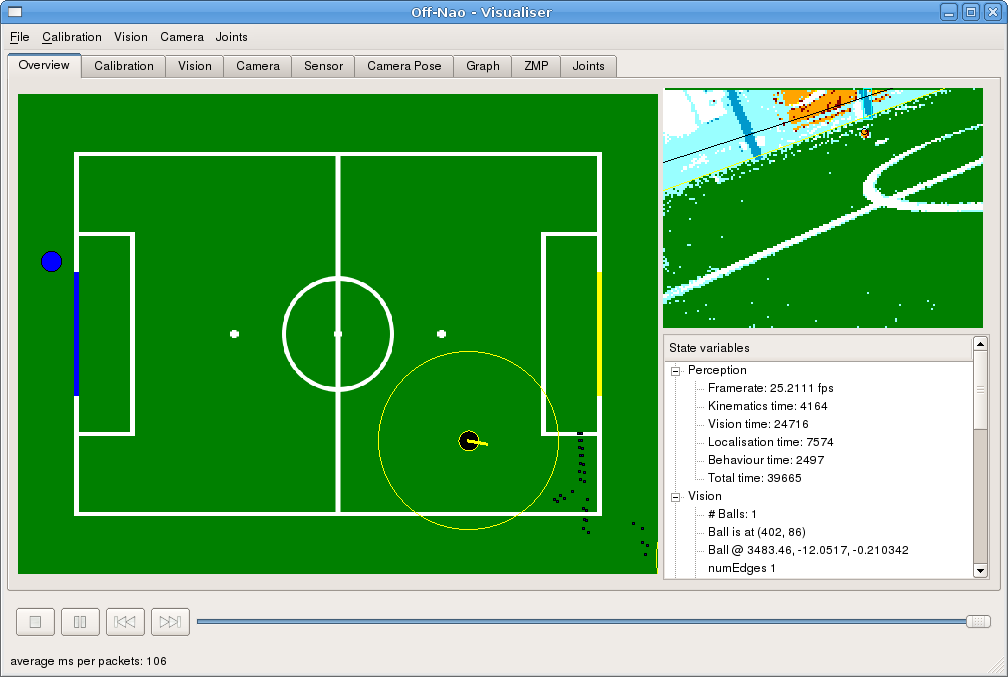
\includegraphics[width=0.5\textwidth]{figures/horizon}
\caption{Black line depicts the horizon. Image taken with Nao leaning to
the side on one foot.} \label{figHorizon}
\end{figure}

The horizon is defined to be the line at an infinite distance and parallel to the y-axis of our robot relative coordinate system (as defined in \autoref{appendixMDH}).  

The steps for calculating this horizon are as follows:

\begin{enumerate}
\item Take two arbitrary points on a line that is at an infinite distance on the ground plane and parallel to the y-axis of the robot relative coordinate system.
\item Using inverse of the cached kinematic transform map these points into camera space.
\item Use field of view of camera to apply a projection matrix to then take these two points into image space. In image space we now know which pixels these points correspond to.
\item Recalculate the line from these two pixels and find the intercept for this line at the left and right sides of the image. These two intercepts are the points we pass to vision so that it may not process pixels that are above this line if not necessary.
\end{enumerate}

\section{Body Exclusion} \label{sectionBodyExclusion}

To ensure that vision does not detect objects such as field lines or balls within the robots own body the kinematic chain is used to determine which parts of the image contain body parts.  This can be seen in \autoref{figKinematicsOverTheShoulder} in which the shoulder is blocking out part of the image.

Ideally, to calculate this we would construct a 3D model of the Nao robot and
then calculate the full kinematic chain to each of these points. This would
require us to calculate the kinematic chain to all limbs on the Nao.

For example, to project points that lie on the right hand into the image, we
need the kinematic chain from the hand to the camera. In contrast, points that
lie on the Nao's upper arm require a smaller kinematic chain that starts at the
shoulder joint and ends at the camera.

An efficient way to accomplish this is to project the points around the shoulder joints onto the image, then once all points around this joint are projected, multiply the matrix chain with a transform that takes us to the joint past the elbow. After this all points about the elbow are projected onto the image. In this way we can repeat a similar process and project the full 3D model onto the image.

However, because of the constraints of our walk and the way in which our behaviours are written, most of this model will never be visible in the camera image. Our primary concern was to ensure we can not see objects within our own chest while looking down at the ball. 

Thus to save on computation only a crude outline of the parts of the body seen from the camera when the robot is in a standing pose are modeled. Because all of these parts are in the torso, we then only have to compute one kinematic chain that extends from the camera to the torso. This again saves on computation.

It was noted however that we occasionally saw our feet in the image. To improve we may look at modeling the feet in future versions.

The vision system uses this information by mapping the body exclusion information gathered into the saliency scan resolution, \autoref{saliencyScan}, allowing the body information to be excluded before a frame is processed.

\section{Nao Kinematics Calibration}
\label{kinematicCalibration}
\begin{figure}[ht]
\centering
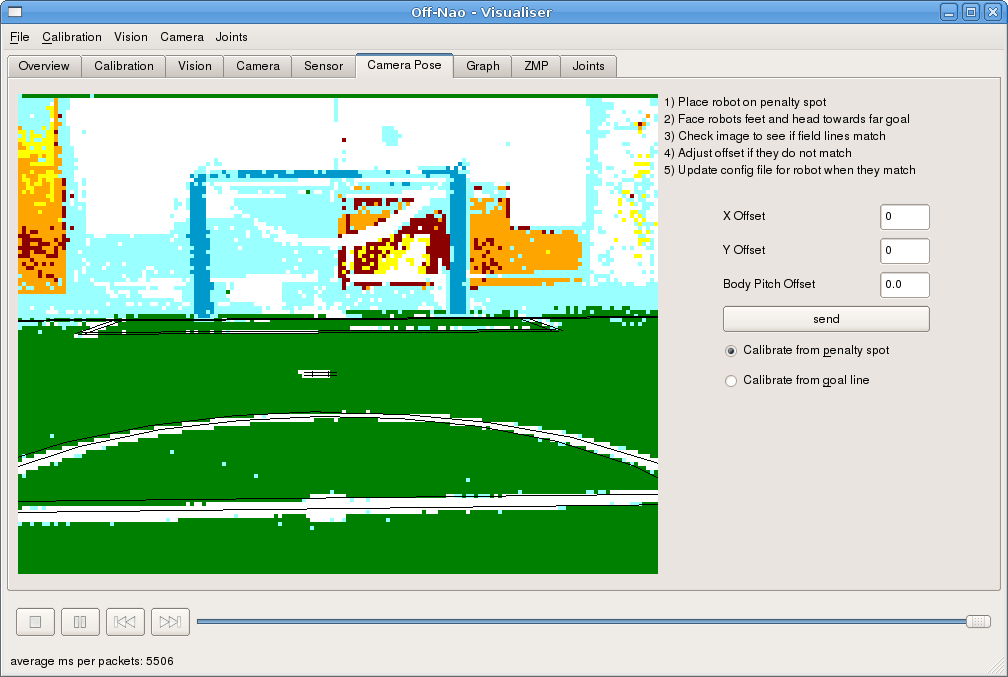
\includegraphics[width=1.0\textwidth]{figures/kinematicsCalibration}
\caption{Image showing a correctly calibrated kinematic chain.} \label{figKinematicCalibration}
\end{figure}


As discussed in \cite{thomas09code}, the Nao robot has physical inaccuracies in
its build such that once we perform the correct kinematic transforms to
determine the distance and heading to objects perceived in a camera frame we
produce a systematic error. This is thought to be primarily caused through small
offsets in the angle of the camera mount. 

To account for this, two offset variables were added to the kinematic chain to account for this camera mount inaccuracy. One variable is an offset in degrees for the pitch of the camera and the other its yaw. A roll offset was also noted on some of the robots but its effect was negligible and due to time constraints was not corrected for.

In addition to this, separate offsets are needed for the top camera and bottom camera. Thus, top and bottom camera offsets must be calibrated for each camera.

A tool in Off-Nao was developed to calibrate these offsets. See \autoref{figKinematicsCalibration}. The process to calibrate is as follows:
\begin{itemize}
\item Position the robot with the back of its feet directly over the back edge of the penalty spot and facing with a heading directly towards the centre of the far goal posts. To ensure this heading was accurate a small rod was used to correct the heading of the robot by placing it between the robots feet and ensuring the robots feet were parallel.
\item Connect to Off-Nao and start streaming images on the Kinematic Calibration Tab.
\item By comparing the projected lines and the actual field lines as seen in the image, adjust the offsets and send them to the robot.
\item View the updated image. If lines still do not match projected lines repeat the last step until they do.
\end{itemize}

Each time we send new offsets to the robot these new offsets are used in the determination of the kinematic chain. This new kinematic chain is then sent to the wireless and used in Off-Nao. Off-Nao takes the inverse of this kinematic chain and uses it to project a map of the field onto the image. In this way we can determine how the offsets need to be changed and the process continues as described above.

\begin{figure}[ht]
\centering
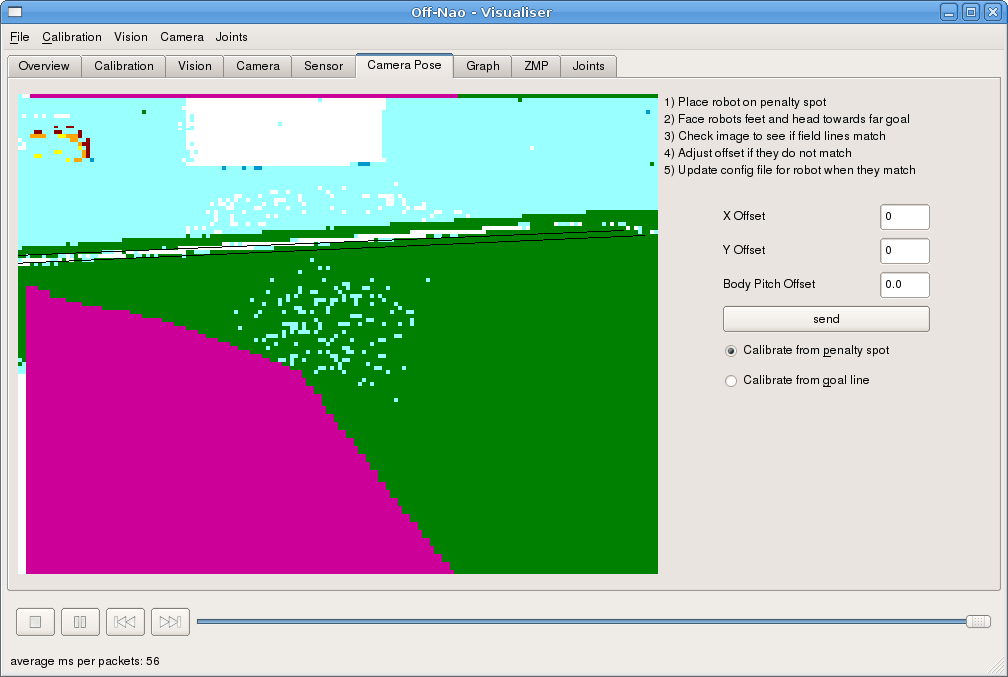
\includegraphics[width=1.0\textwidth]{figures/kinematicsOverTheShoulder}
\caption{Image showing how the field lines projected via the kinematic chain may sometimes not match the actual field lines when looking over the shoulder.} \label{figKinematicsOverTheShoulder}
\end{figure}


It was also noted, when performing this calibration process that when looking over the shoulder to calibrate we get inaccurate distances. This was later attributed to a `body offset'. The body offset encompasses further inaccuracies in the build of the robot and is used to approximate those in order to correct for this effect. This parameter was not successful in fixing this issue and for some robots it was extremely hard if not impossible to come up with a set of parameters that would result in the field lines being projected correctly when looking forward and when looking over the shoulder. See \autoref{figKinematicsOverTheShoulder}.

A project is already underway for next year in which we aim to automatically calibrate these offsets using a gradient hill climbing method.

\begin{notesfornextyear}
\section{Nao Camera \& video4linux}
In the first iteration of the rUNSWift Nao teams, images were retrieved from
the camera using the supplied NaoQi interface.  At the time, this involved
NaoQi reading a set number of bytes from the camera interface, processing it to
be in a requested format (such as RGB), and then being copied to the
runswift module.  Simply retrieving a 320x240 image in this manner and keeping
it in the native camera format of YUV422 used 35\% of the CPU.

video4linux was used to directly access the camera device and obtain the
images.  In doing so, the 2008 rUNSWift team noted that the camera provided
with the Nao V1 and Nao V2 did not support memory maps or user pointers, and
that the camera could be read as a normal file, using only 18\% of the CPU for a
320x240 image, or 78\% for a 640x480 image. \cite{videodevice} However, the code
for using memory maps or user pointers was left in place.

The 2009 rUNSWift team was later able to use memory maps to access the camera
images with the Nao V3, thereby requiring near-zero CPU usage.  When Aldebaran
provided the appropriate ioctl calls, capability to switch between the two
cameras on the Nao was added.  However, it was found that, to eliminate
shearing of consecutive images with the memory maps, streaming had to be
disabled when switching cameras.  This is not necessary when using read
system calls.
\end{notesfornextyear}
\section{Colour Calibration and Camera Settings}
\label{sec:camcolcalib}
Camera settings are vital to the overall performance of the vision processing system as they have a dramatic influence on the ease of colour calibration and the amount of blurring. While an automatic tool was planned for the competition (see \autoref{sectionCameraCalibration}), the camera settings were chosen manually using the Telepathe tool. This involved setting the exposure as low as possible in order to lessen the amount of blurring, but high enough so that there is enough contrast in the image for the colour calibration to separate the colours with minimal misidentification. 

The other important step to calibrate our vision system for use in a particular venue is colour calibration. The different colours calibrated are: \begin{itemize}
\item{Orange: This colour is used to calibrate for the orange ball used in the competition}
\item{Field Green: Represents the green of the field}
\item{White: Represents both the field lines and parts of the robot}
\item{Goal Yellow: Represents the yellow coloured goal}
\item{Robot Red: Represents the pink band worn by robots on the red team}
\item{Goal Blue and Robot Blue: Represents both the blue goals and the blue bands worn by robots on the blue team. While it was originally intended that these would be separate colours, it was found that the colours was too close to each other to reliably classify them as independent colours}
\item{Black: Spare colour that can potentially be used for an item seen in the background to stop it being calibrated as one of the major colours}
\item{Background: This was used to represent areas of the saliency scan image covered by the robot's own body}
\end{itemize}

The colours are calibrated by taking recordings from several different robots due to slight differences in the colours recorded by each camera, even using the same camera settings. The colour calibration tool uses a simple weighted kernel classification algorithm developed by \cite{kimcuongpham}: each training sample increases a weighting for that particular YUV value toward the classified colour. Neighbouring values in colour-space, within a fixed Euclidean radius, also have their weights increased, at an exponentially decreasing rate, giving generalisation. The kernel file can then be used to generate a constant-time lookup table for use on the robot at runtime.

\section{Saliency Scan and Colour Histograms \label{saliencyScan}}

To maximise the amount of information available to the state estimator, it is
desirable to ensure the vision system can run at 30 frames per second, as this
is the maximum rate at which the Nao's camera can capture images. Unfortunately,
on the Nao's hardware, is is impractical to colour classify an entire 640x480
pixel image and scan for features such as balls, goals, robots, etc. whilst
maintaining a 30 frame per second processing rate. As a trade-off, the first
step of the rUNSWift vision pipeline is to subsample the image down to a 160x120
pixel resolution, and colour classify those pixels. While this is done,
histograms in the x and y-axes for each of the major field-space colours are
generated. The maxima of these histograms can be found efficiently, allowing
the rest of the vision system to analyse only the most interesting parts of the
image at the native resolution.

Still, the creation of the saliency image is a cpu-and-memory-consuming process,
and needed to be heavily optimised.  Analysing the compiler-generated assembly
code in this regard was invaluable.  The main optimisations attempted were:
\begin{itemize}
  \item Reducing the amount of memory used
  \item Reducing the number of memory accesses
  \item Reducing the number of local variables used (thereby reducing the
number of variables in memory)
  \item Reducing the number of calculations performed in accessing array by
using pointer arithmetic instead of array indexing
\end{itemize}
\begin{notesfornextyear}
A more detailed list of optimisations:
\begin{itemize}
  \item The histogram data was always stored as 16-bit integers, as the
saliency image is parameterised to be as big as 640x480.  It was changed to
use 8-bit integers if the image was smaller than 256x256.
  \item Rather than keeping variables to designate the indices into the
saliency image and then iterating through valid values for the indices, a
pointer was kept to the active pixel in the saliency image and that
pointer was iterated through the entire image.
  \item Rather than reading each channels of each YUV pixel as three individual
8-bit bytes, the entire 32-bit word containing two VYUY pixels is read, and
unused information is removed, thereby requiring one memory access instead of
three.
  \item Our colour classification table is a 2MB 128x128x128
YUV-to-classified-color lookup matrix.  This is now converted to a 16MB
256x256x256 VYU-to-classified-color lookup matrix.  (The conversion is done at
startup time and is quite costly and unoptimised.)  The reason for doing this is
so that the conversion from a 32-bit word containing two VYUY pixels to a
classified colour can be done in two assembly instructions.
  \item Rather than storing histogram data for all colours, we only store
histogram data for the colours where the histogram is used, i.e. blue and yellow.
 This requires us to perform a comparison and a conditional branch of every
classified pixel, but saves us from performing memory accesses to update the x
and y histograms.
\end{itemize}
The changes made are shown in \vref{saliencyScanCode}.

The recommended future extension is to write this function in assembly, as the
compiler does not choose optimal variables to keep in registers, specifically
the address of the colour classification table.  Another extension is to optimise
the colour classification table generation.
\end{notesfornextyear}

While the saliency scan is being built, the body exclusion information, as seen in \autoref{sectionBodyExclusion} is used to remove the robot's own body from the saliency image. The saliency scan is provided an array of coordinates that define the lowest coordinate in each column of the image that is known not to contain the robot's body. Therefore, the saliency scan is filled down a column as normal until this coordinate is reached. All pixels in the saliency scan below this coordinate in the column are marked as the Background colour. This means that any processing performed on the saliency scan later in the vision processing pipeline can stop scanning down a column whenever a Background coloured pixel is seen.

\label{secFieldEdgeDetection}
\section{Field-Edge Detection}
After generating colour histograms, to further reduce the amount of high-resolution scanning to be done in vision, and to assist with localisation, the edges of the green field are detected. In 2009 B-Human used a convex hull algorithm to exclude areas above the field edge \cite{thomas09code}, which achieves the first goal of reducing the area of the image to be processed. In 2010 rUNSWift used a similar method of vertical scanning to detect points on the edge of the field, but rather than a convex hull algorithm, multiple iterations of the RANSAC algorithm was used to find straight lines. When two field edge lines are detected, the possible positions of the robot are reduced to 4 hypotheses.

Initially the first green pixel in each column of the saliency scan is recorded, by scanning vertically from the horizon down. This mostly eliminates false edge points from distant fields and green clothing in the background. See \vref{fig:EdgeDetection_OneLinePoints}.

\begin{figure} [t]
\centering
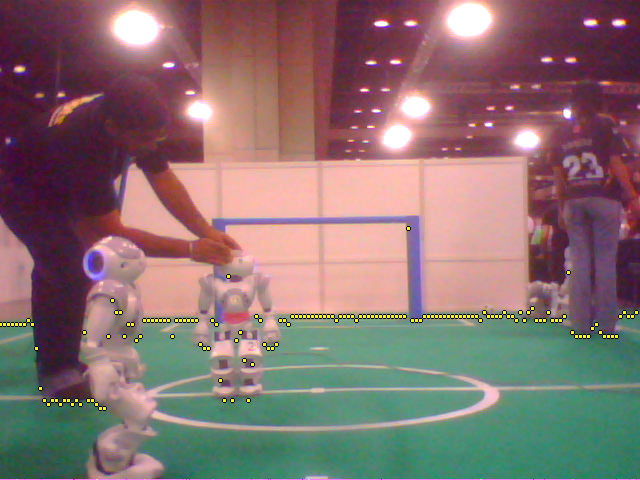
\includegraphics[width=1.0\textwidth]{figures/EdgeDetection_OneLinePoints}
\caption{Candidate points for a field-edge line} \label{fig:EdgeDetection_OneLinePoints}
\end{figure}

Secondly, the RANSAC algorithm chooses the parameters for a line in $t_1x + t_2y + t_3 = 0$ form, to maximise the number of points that fit a line. See \vref{fig:EdgeDetection_OneLinePointsAndLine}.

\begin{figure} [t]
\centering
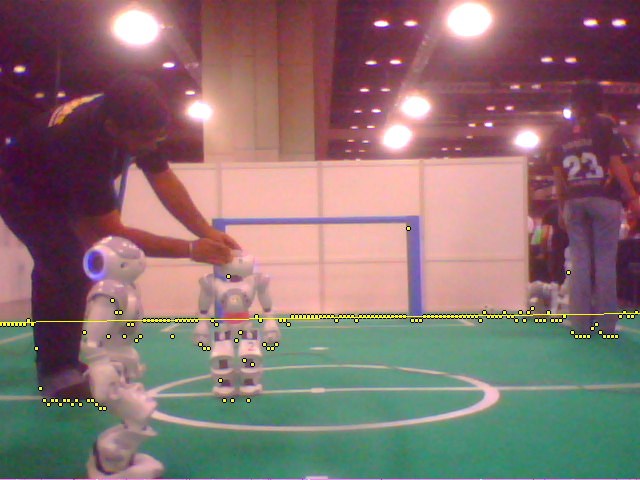
\includegraphics[width=1.0\textwidth]{figures/EdgeDetection_OneLinePointsAndLine}
\caption{Line found by performing RANSAC on the candidate points} \label{fig:EdgeDetection_OneLinePointsAndLine}
\end{figure}

Finally, the consensus set of the first line is removed from the candidate points, and RANSAC is repeated, possibly finding a second line. See \vref{fig:EdgeDetection_TwoLines}.

\begin{figure} [t]
\centering
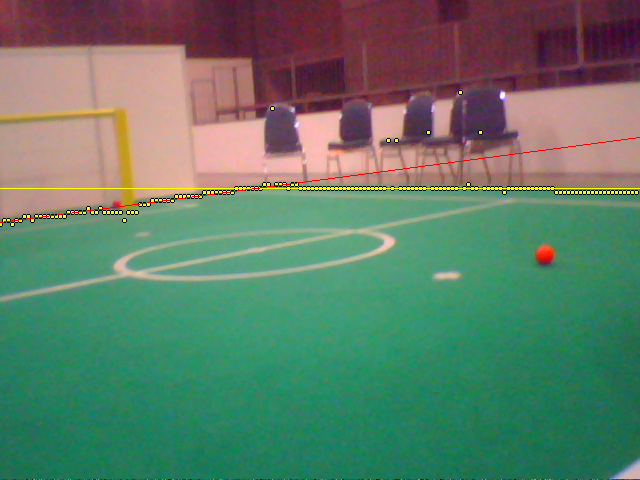
\includegraphics[width=1.0\textwidth]{figures/EdgeDetection_TwoLines}
\caption{Lines found by performing RANSAC twice on the candidate points} \label{fig:EdgeDetection_TwoLines}
\end{figure}

A slight modification to our edge detection algorithm was implemented at the competition to allow it to work properly when adjacent fields are also seen in the frame. While this was ultimately not needed as barriers were put in place between fields, our modification enabled the field edge detection to work when neighbouring competition field can be seen. Initially, as our field edge detection algorithm scans down a column until the first field green pixel is seen, this meant the field edge was often placed at the edge of the neighbouring field. Aside from directly affecting localisation due the field lines being placed in the wrong position, balls, robots and field lines could all be detected on other fields.

To prevent this happening, the small border around the field was calibrated as
black, and the scan down each column was modified. Instead of reporting the
first green pixel encountered in the column, the top most green pixel not above
a black pixel was reported. This technique successfully allowed us to reliably
eliminate issues with seeing other fields in the same frame.

\section{Region Builder}
The region builder identifies potential areas of interest on the field, providing the first stage of processing for the ball detection, field line detection and robot detection. It operates by firstly identifying regions in the image, and then using the colour of pixels and shape of regions to identify what each region most likely represents. In order to achieve this, several statistics about the regions are generated as a region is built. A region contains information such as: \begin{itemize}
\item{The number of pixels of each colour in the region}
\item{Coordinates of the bounding box of the region}
\item{Coordinates of the bounding box of robot colours in the region}
\item{The number of runs in the region that started at the field edge}
\item{Whether the region has been removed from further consideration}
\item{The average length of the runs in the region}
\item{The start and end y coordinate of the last run added to the region. This is used only during the region building process}
\item{The column index of the right-most robot red or robot blue coloured pixel in the region. This is used only during the region building process}
\item{The start and end coordinates of all runs that make up the region}
\item{The type of object the region could possibly be}
\end{itemize}

\subsection{Region Detection}
As the ball and the field lines will be in the frame below the field edge, as well as a portion of other robots, the region builder only scans below the field edge. Being the first stage of processing for the majority of the feature detection, the region builder operates only on the saliency scan to save processing time. Each column of the saliency image is scanned to identify runs of non field-green pixels. A \emph{run} starts when either a orange, white, robot red or robot blue pixel is found, or when an unclassified pixel is found at the start of the column scan. The special case is made for unclassified pixels as a robot's leg can offer appear completely unclassified. For runs starting with orange (ball coloured) pixels, the run will finish when either a green, white, robot red or robot blue pixel is found, when a few unclassified pixels are found, or when the bottom of the image is reached. Alternatively, for runs starting with other colours, they will finish when either an orange pixel is found, when more than one green pixel in a row is found, or when the bottom of the image is reached. If a run contains only unclassified pixels and is less than 10 pixels, it is deleted to stop slight errors in the field edge position from being considered as regions.

Once a run is finished, information about the run is used to build regions. A run is connected to a region only if the following conditions are met: \begin{itemize}
\item{If the last run added to the region was from the column before the current run}
\item{If the y coordinates of the last run added to the region cover at least one of the y coordinates of the current run. This test and the previous test ensure that the run touches the existing region}
\item{If the region contains orange pixels, the run will only be connected if it also contains orange pixels. Similarly, if the region contains no orange pixels, the run will only be connected if it also contains no orange pixels. This test is to split potential ball regions from potential field line and robot regions}
\item{If the run contains robot coloured pixels and the region does not, they are only joined if the region is less than a certain width. A larger threshold for the width is used if the run started at the field edge. This condition is used to separate regions containing robots and regions containing field lines touching the robot}
\item{If the run contains no robot coloured pixels and the region does, they are only joined if the difference between the x coordinate of the current run and the x coordinate of the right most robot coloured pixel in the region is less than a certain threshold. A larger threshold for the width is used if the run started at the field edge. As with the last condition, this is used to stop robots and field lines from being combined into the same region}
\item{If the length of the run if between half the average run length of the region so far and double the average run length of the region so far. This is a further condition to separate regions containing robots and regions containing field lines}
\end{itemize}
If all these conditions are met, the run is connected to the region and all the information about the region is updated with the current run. However, if no region is able to meet all these conditions, a new region is created for the run, and added to an array of regions identified in the frame. As the naive approach to scan through all the regions so far created to test if they can be joined with a run is computationally very expensive, an optimisation is performed to allow this step to operate in constant time. An array of pointers to regions containing runs from the previous column is stored. Using the conditions for joining a run to a region listed above, any potential regions that could be joined are contained in this array. Furthermore, the array is sorted in order of increasing starting y coordinates of the previous run. Therefore, when the array is searched to find a potential region, the array only needs to be searched until the starting y coordinate of the last run in the region is further down the image than the ending y coordinate of the current run. 

If the next run to be potentially combined is in the same column, the search through the array can start where the previous search finished because the next run will always be further down the image than the current run. As each run in a column is either combined with an existing region or used to create a new region, a pointer to this region is stored in a separate array. When all the runs from a column have been processed, this array can then be searched so that runs from the next column can be combined with regions, as the array will already be in the correct order. This processing is summarised as follows:

\begin{algorithmic}
    \FORALL{$column\ \mathbf{in}\ saliencyScan$}
    \FORALL{$row\ \mathbf{in}\ column$}
    \IF{have reached the end of a $run$}
    \FOR{$reg\ \mathbf{in}\ lastColumnRegions$}
    \IF{$reg.startY > run.endY$} 
    \STATE{\bf{continue}}
    \ENDIF
    \IF{$reg.endY \ge run.startY$}
    \IF{conditions for joining $run$ to $reg$ are met}
    \IF{$run$ hasn't been joined to a region yet}
    \STATE{Join $run$ to $reg$}
    \STATE{Add $reg$ to end of $thisColumnRegions$}
    \ELSE
    \STATE{Merge $reg$ with previous region $run$ joined}
    \ENDIF
    \ENDIF
    \ELSE
    \STATE{$\mathbf{remove}\ reg$ from $lastColumnRegions$} 
    \ENDIF
    \ENDFOR
    \IF{$run$ has not been joined to a region}
    \STATE{Create new region for $run$}
    \STATE{Add new region to $thisColumnRegions$}
    \ENDIF
    \ENDIF
    \ENDFOR
    \STATE{Set $lastColumnRegions\ =\ thisColumnRegions$}
    \STATE{Set $thisColumnRegions.size\ =\ 0$}
    \ENDFOR
\end{algorithmic}

If a single run can be connected to more than one region, all the regions that it can be connected to are joined together. This can be achieved fairly simply while a run is being added to a region. When searching through the array of pointers to regions containing runs from the previous column, if a region is found that meets all the conditions above, the information about the run is added to the region. After this, the search through the array continues until the starting y coordinate of the last run in the region is further down the image than the ending y coordinate of the current run. Any region found in the array during this search that also meets all the conditions above is combined with the regions so far joined. All the information from one of the regions is added to the other, and the former region is marked as deleted. The region is only marked as deleted because removing it from the array of all regions in the frame is unnecessarily expensive. 

Note that an array of fixed length is used instead of a list to store all the regions in a frame to avoid having to allocate large amounts of memory in the heap in each frame. Additionally, it is more efficient for later processing of the regions if they are stored in ascending order of their left most run. As the columns are scanned left to right across the frame, the array will be in this order as it is formed. To ensure that this order is maintained when combining two regions, the region that does not have the left most run is deleted. The output of the region detection is shown in \autoref{fig:RegionBuilder1}.

\begin{figure} [t]
\centering
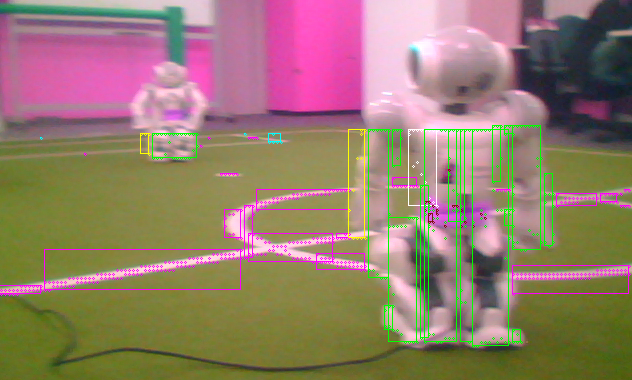
\includegraphics[width=0.7\textwidth]{figures/regionScreenshot1.png}
\caption{Regions identified during the region detection process} \label{fig:RegionBuilder1}
\end{figure}

\subsection{Region Merging and Classification}

During the region building process, several checks are used to separate regions containing field lines and regions containing robots. However, a drawback of this is that robots are often split into several regions. Once the region building process is complete, all the regions identified are scanned to determine if they most likely represent a robot, field line or ball, so that they can be used used by the robot detector, field line detector and ball detector respectively for further processing. Regions can also be deleted if they could potentially be noise, such as noise from an error in the field edge. During this classification, regions that potentially represent parts of a single robot are added to a robot region. Robot regions are simply a specialised type of a region that hold similar information as standard regions, and are formed by adding one or more regions to the robot region. This process is aims to combine the several small regions that cover a robot into a larger region. 

In order to do this, the array containing the region information is scanned from left to right. Any region containing ball colours is considered to be a possible ball and plays no part in the robot region building process. A robot region is created when a region that contains either robot red or robot blue is found. It is also possible for a robot region to be created if a region is found where the majority of columns in the region contain runs that start at the field edge, and if the average length of the runs in the region is more than half the height of the region. This third condition for creating a robot region is needed because it is possible for a robot's band to be above the field edge in the image. After a robot region has been created, regions are conditionally added to the robot region until a region is found whose left most coordinate is greater than the right most coordinate of the robot region, or if the region contains a different robot colour to the robot region. This takes advantage of the fact that the array of regions is sorted according to the left most coordinate of each region. The condition for adding a region to the robot region is that the region must satisfy at least one of the following properties: \begin{itemize}
\item{If the region contains some robot coloured pixels. However, if the region contains all robot red, with no white and is entirely below the current bottom most coordinate of the robot, it is deleted as it potentially could represent a badly classified ball}
\item{If the region contains more than one run that started at the field edge and is taller than it is wide}
\item{If more than two thirds of the columns in the image contain runs that started at the field edge}
\item{If the region is completely contained inside the robot region}
\item{If the region is taller than it is wide, doesn't extent far beyond the current bottom of the robot and the average length of the runs is greater than half the height of the region}
\end{itemize}
During this process, regions that are though not to contain any useful information, such as regions formed due to errors in the field edge, are marked as deleted. The conditions for this to occur are: \begin{itemize}
\item{If the region is less than three pixels wide and cannot be joined to a robot}
\item{If the region touches either the left or right edge of the image, is taller than it is wide, and the average length of the runs is more than one third the height of the region. This is designed to prevent cases where a small part of a robot, such as some of the arm of the leg, is just seen in the edge of the image from being mistakenly reported as field lines}
\item{If the region is completely below a robot region and contains some robot red. This is to prevent a small bit of robot red in a ball from being joined to the robot region}
\item{If the region contains runs that started at the field edge, but has a height less than 10 pixels}
\end{itemize}
This process is not quite enough on its own to successfully combine all regions representing a robot in a robot region. When a potential robot region is created, the next regions in the array are examined to see if they should be added to the region, as described above. This is successful in adding small parts of robots, such as parts of the arm or leg that by themselves don't look like a robot, to the robot region, as they can often get separated from the region that contains enough information to be identified as a robot. However, this only works for regions that start to the right of the region initially identified as a robot. In order to allow regions that start to the left of the region initially identified to be added to the robot region, the array of regions and the array of robot regions are scanned concurrently in reverse order - each iteration of the loop decreases the counter for the array of regions by one. If the current region's left most coordinate is lower than the current robot region's right most coordinate, the counter for robot regions is decreased. The current region is added to the current robot region if: \begin{itemize}
\item{The region overlaps the left side of the robot region, and}
\item{The region is taller than it is wide, and}
\item{The region contains some runs that started at the field edge or the average length of the runs in the region is more than half of the height of the region}
\end{itemize}
All the regions that have not been marked as deleted, identified as possible balls or combined into robot regions are considered to represent field lines. At this point, vertical field lines that extend from the field edge to the bottom of the frame, can occasionally be incorrectly identified as possible robots, and added to a robot region. The final stage of the region builder is therefore to scan through the robot regions and identify if there are any robot regions that contain no robot colours, touch the bottom of the frame and are less than 50 pixels wide. If such a robot region is found, all the regions that were added to the robot region are considered to represent field lines. The result of this processing can be seen by comparing \autoref{fig:RegionBuilder1} with \autoref{fig:RegionBuilder2}. At this stage, the ball detection, field line detection and robot detection sections of vision can use this region information for further processing.

\begin{figure} [t]
\centering
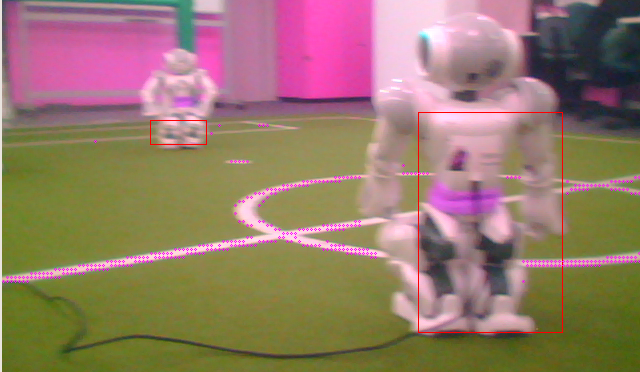
\includegraphics[width=0.7\textwidth]{figures/regionScreenshot2.png}
\caption{Regions identified during the region detection process after the robot regions have been grown} \label{fig:RegionBuilder2}
\end{figure}

\section{Field-Line Detection} \label{sectionFieldLineDetection}
The field line detector identifies the coordinates of pixels on the edge of field lines and translates the image coordinates into robot relative coordinates. This information can then be matched to a map of the field, as described in \autoref{sectionFieldLineUpdates}. Much of this information has already been collected during the region building process. Each region contains a list of the start and end coordinates of each run in the region. As runs are a vertical sequence of non-green classified pixels, the start and end coordinates of each run in regions identified as containing field lines can be used as the edge points of field lines. In directly using the information generated during the region building process, the field line detection can run extremely fast. It should be noted however that as the region builder only operates on the saliency scan, each individual edge point has a small error. However, as multiple edge points are used during the field line matching process, these slight errors were not large enough to cause a noticeable deterioration in localisation, so it was not considered to be worth the additional processing expense to make the line edge points accurate to one pixel in the full resolution image.

As the run time performance of the field line localisation search deteriorates rapidly with increasing numbers of edge points, the maximum number of edge points reported is 40. To ensure the selected edge points are distributed evenly throughout the frame, total number of runs in all field line regions is calculated (each region stores the number of runs it contains). From this, the number of runs to skip between edge points being added can be simply calculated. The final step in the field line detection process is to scan through the list of edge points of each line region, skipping the calculated number of edge points each time, convert the chosen edge points to robot relative coordinates and write these to the blackboard.

\section{Robot Detection}
The robot detection algorithm is split into two parts. The first further processes the robot regions detected in the region builder and performs additional sanity checks, and is run before the ball detection and the goal detection to provide these components with the image locations of likely robots for their own sanity checks. The second performs additional sanity checks and converts the robot region to robot relative coordinates for reporting to the blackboard. This split is to allow other components of vision, such as ball detection, to remove possible balls if they are inside robots, while allowing the robot detector to also use the ball detection and goal detection for sanity checks. Performing additional sanity checks in the first stage of robot detection instead of at the end of during the building of robot regions in the region builder also reflects the different aims of these sections: the region builder focuses on ensuring that no regions that could possibly be a part of a robot end up being classified as field lines, leading to some false positives for robots, while the robot detection focuses on reporting as few false positives as possible.

\subsection{Initial Robot Detection Processing}
The first stage of the robot detection uses a series of sanity checks to remove false positives from the robot region information. Robot regions are removed from further consideration if: \begin{itemize}
\item{If the top of the robot region is below the field edge}
\item{If the number of scans in the robot region that started at the field edge is less than one third of the robot region's width}
\item{If the robot region is less than a threshold  minimum width}
\item{If the number of white pixels in the robot region is less than a threshold minimum}
\item{If the robot region spans the entire height of the image, yet takes up less than a third of the width of the frame and is not on either the left or right side of the image. This is to remove near vertical field lines from being considered robots in some cases}
\end{itemize}
Up to this point, robot regions can still exist even if no robot blue or robot red pixels are contained in the region, as often the coloured band worn by a robot can appear above the field edge in an image. Therefore, if there are less than a threshold number of robot coloured pixels in the robot region, the area of the image directly above the robot region is searched for robot colours. As with the region builder, the search is performed on the saliency scan. The search is performed by scanning rows of the saliency scan, starting from the row above the top most row in the robot region. Each scan starts from the left most of the robot region to the right most of the robot region. The search continues until either a threshold number of rows have been searched, or a robot coloured pixel is found. If a robot coloured pixel is found, a threshold number more pixels have to be found in the following two rows for a robot of a particular colour to be reported.

A second list of robot regions stores the reduced number of robot regions that have been detected. If the robot colour of a robot region has been found, and is either a different colour to the previous robot region added to the new list, or is not adjacent to the previous robot region added to the new list, it is added to the list. Otherwise, if the colour of the robot region has been found, and is the same colour as the previous region added and is adjacent to the previous region, it is combined with the previous region. Additionally, if the colour of a region has not been found, it is combined the previous region in the list if they are adjacent to each other, otherwise it is deleted. This extra step to further combine robot regions (in addition to the combining process in the region builder) is taken because occasionally a pixel in the robot's joints is classified as a robot colour, which creates separate regions if the colour of the robot is different. The sanity checks in the robot detector should remove these small regions, and allow the remaining regions to be properly combined.

Finally, the robot regions that were removed by the sanity checks at the start of the robot detector are examined to see if they can be joined to any confirmed robot regions. While this does not create any new confirmed robot regions, it can expand the dimensions of existing robot regions, which can make some sanity checks in the ball detection (removing balls from inside robots) and goal detection (stops goals from being removed if their bottom is above the field edge, but they are above a robot region).

\autoref{fig:robotDetection} shows an example of the robot detection, where the bounding boxes around each robot region is coloured to reflect the detected colour of the robot's band. It can be seen in this screenshot that the band of two of the robots is above the field edge.

\begin{figure} [t]
\centering
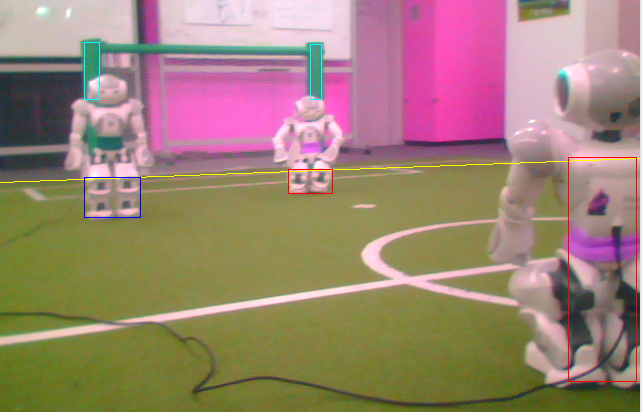
\includegraphics[width=0.7\textwidth]{figures/robotDetectionScreenshot.png}
\caption{The bounding box around robot regions identified in the image} \label{fig:robotDetection}
\end{figure}

\subsection{Final Robot Detection Processing}
The second stage of robot detection uses more sanity checks to lessen the likelihood of reporting false positives, and converts the robot region information to robot relative coordinates. The sanity checks here remove robot regions if: \begin{itemize}
\item{If the robot region is thought to represent a blue robot and the bounding box of the robot blue coloured pixels in the robot region is contained within the bounding box of a goal post identified by the goal detection. This sanity check is used to prevent goals from being reported as robot regions, and is especially needed because the goal blue and robot blue are not separately classified}
\item{If the robot colours are all to one side of the robot. That is, if all the robot colours in the left fifth or right fifth of the robot region. This is also designed to prevent goals from being reported as robot regions}
\item{If the robot colours are contained within the bounding box around a ball identified by the ball detection. This is used as often some pixels in the ball can be classified as robot red. If the ball is close in the frame to the robot, this can affect the determine of the side of the robot, particularly if the robot's band is not in the frame}
\item{If the team of the robot region has not been identified. Only robot regions that are thought to contain red robots or blue robots are reported}
\end{itemize}
Finally, the image coordinate of the middle of the bottom of the robot region is used to calculate the robot relative position of each robot. A boolean value is also calculated to store if the robot region touches the bottom of the image --- in this case, the robot relative distance to the robot will likely be incorrect. This position and boolean value is written to the blackboard for each robot detection.

\section{Ball Detection} \label{sectionBallDetection}
The ball detection uses the regions identified in the region builder as being possible balls to locate the mostly likely position and size of the ball in the image, and then uses edge detection to identify the outline of the ball as accurately as possible. Firstly, the regions that have been classified as possible balls are scanned and the one which satisfies two sanity checks and contains the largest number of pixels is chosen to be the region that the ball detection will examine. The two sanity checks are failed if: \begin{itemize}
\item{If the ball region is inside a robot region. To prevent balls at the feet of a robot from possibly being removed by this sanity check, if the ball region covers only the lower part of a robot region, the sanity check passes, unless the robot region extends to the bottom of the image.}
\item{If the ball region could be due to background noise caused by a slight error in the field line. At times, when there are a lot of obstructions on the field preventing the field line from being clearly seen, such as from other robots and referees, or when a corner of the field is seen near the edge of the image, the field edge can be placed on the image above the actual edge of the field. When this occurs, any orange in the background below the field edge can potentially be reported as a possible ball. This can become a particular problem when there are people around the field, with orange shoes, feet and arms potentially being detected as possible balls. To test for this, a vertical scan line from the middle of the top of the region to the horizon is tested to see if it contains a green pixel. If it does, it is assumed the region is not from background noise. Otherwise, a scan line is used to look for green pixels in the other three directions away from the region. If there are no field green pixels found within 10 pixels away from the region in more than one of the three directions, and the region contains less than 100 pixels, the region is considered to be background noise and the sanity check is failed}
\end{itemize}

\subsection{Edge Detection}

If a region containing more than one pixel is found, the next step in the ball detection is to use edge detection to find a list of pixels on the edge of the ball. To make this process as efficient as possible, three different resolutions are used depending on how many pixels are in the ball region --- the less pixels in the ball region, the smaller the ball is likely to be in the image, so a higher resolution is needed to find enough pixels on the edge of the ball for further processing. Additionally, in order to make more efficient use of the information already gained in the region builder, a slightly different algorithm is used for the two most coarse resolutions used. In both cases, the full resolution image is used to find the edge points.

If the ball region is less than 15 pixels, the ball is most likely very small in the image, so the highest resolution is used to scan for edge points. In this process, every column between the left most and right most extent of the region is scanned upwards from the middle y value of the region (the midpoint between the top and bottom most pixels in the region). The scan for a column finishes when either an edge, green classified pixel or white classified pixel is found. A pixel is considered to be an edge when the \emph{v} channel of the pixels immediately before and immediately after the current pixel differ by more than a threshold amount. This was found to give more accurate results than using the absolute differences between the \emph{y, u}, and \emph{v} channels because the brightness of the ball tends to change quite markedly near the edges, causing the edge detection to often find edges inside the ball. The scans also stops when either green or white classified pixels are found as these two colours are commonly seen around the ball, and it is very unlikely that a pixel inside the ball will be classified as white or green. This allows the ball edges to be found even when the edge detection fails, such as when the ball is significantly blurred.

After points on the top of the ball edge have been found, the same procedure is used to find pixels on the bottom edge of the ball, by scanning downwards from the middle y value of the region. Each row between the top and bottom most pixels in the original region is also scanned to the left and right of the middle x value of the region. As previously, the scans stop when either an edge, white pixel or green pixel is found.

Alternatively, if the ball region is greater than 15 pixels, the start and end coordinates of each run in the region, as found and stored by the region builder, are used to speed up the scan for the pixels on the ball edge. The pixels on the top and bottom edges of the ball are found by scanning through the list of start and end coordinates of each run. For a given start coordinate, the corresponding coordinate in the full resolution image is found (the region builder uses the saliency scan), and this column is scanned for the top edge of the ball. The scan starts a few pixels below the start coordinate, and continues upwards until either an edge, green pixel or white pixel is found. The same method is used to find the bottom edge of the ball, only the end coordinate of each scan is used. In doing so, every forth column is scanned, and the scans only start at the approximate location of the edge, saving considerable processing time. Additionally, if the ball region contains more than 150 pixels, the start and end coordinates of every second run in the region is used, effectively causing every eighth column to be scanned. 

During this process, if the run's x coordinate is one pixel to the right of the left most pixel in the region, or one pixel to the left of the right most pixel in the region, the y coordinate of the top and bottom ball edge point found is recorded. From this, the furthest up the image of the top edge points and the furthest down the image of the bottom edge points recorded can be easily found. These are used as the range of rows to be scanned to find the left and right edge points of the ball. The range is not selected by simply looking at the top and bottom most coordinates of the region to avoid duplication of the ball edges in the areas of the ball's edge that can be found by both horizontal and vertical scans. The left edge points of the ball are therefore found by scanning rows starting from a few pixels inside the left most pixel in the region and stopping when either an edge, green pixel or white pixel is found. The right edge points are found in a similar manner. If the ball region is less than 150 pixels, every fourth row is scanned, otherwise every eighth row is scanned.

\autoref{fig:ballDetection} shows an example of the edge detection being used to accurately identify a ball. The left hand image shows the colour calibrated image, where it can be seen that a substantial part of the ball is unclassified (note that unclassified colours appear as light blue in the screenshot). The right hand image however shows that the edge detection has enable the edge of the ball to be precisely located.

\begin{figure} [t]
\centering
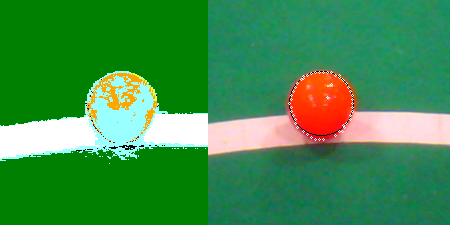
\includegraphics[width=0.7\textwidth]{figures/ballDetectionScreenshot.png}
\caption{A screenshot of the ball detection. The left image shows the colour calibrated image, while the right shows the edge points identified and the circle fitted to the edge points} \label{fig:ballDetection}
\end{figure}

\subsection{Identification of Ball Properties}

Once a list of pixels on the edge of the ball has been found, the centre and radius of the ball can then be calculated. As at least three pixels are needed for this process, if less than three pixels on the edge were found, the ball detection stops and no ball is reported. Otherwise, the ball centre and radius can be calculated by using the following method, a shown in \autoref{fig:ballCircleAlgorithm}: \begin{itemize}
\item{The unique pixels on the edge of the ball are randomly selected}
\item{The equation of a line joining the first and second pixels is found, as well as a line joining the second and third pixels}
\item{The equation of the perpendicular bisectors of both of these lines is found}
\item{The centre of the ball is the intersection of the perpendicular bisectors}
\item{The radius of the ball is the distance from the centre of the ball to one of the three pixels on the edge of the ball}
\end{itemize}

\begin{figure} [t]
\centering
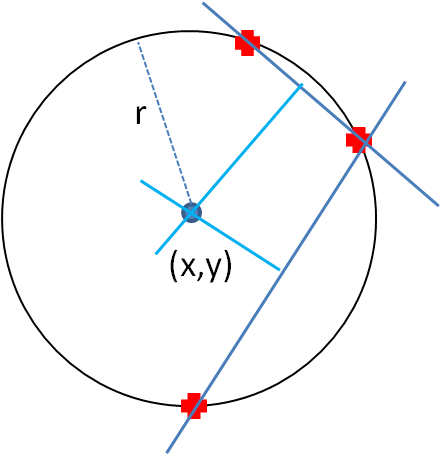
\includegraphics[width=0.5\textwidth]{figures/ballCircleAlgorithm.png}
\caption{The algorithm used to find the centre point and radius of the ball} \label{fig:ballCircleAlgorithm}
\end{figure}

This procedure is repeated 40 times, where each time a different set of three unique pixels is randomly selected. The x and y coordinates of the centre, and the radius found in each run are stored in separate lists. At the end, each of these three lists is sorted, with the aim of finding the median of each of the lists. However, it was found that in cases where a perfect outline of the ball is not found (such as when the ball is half obstructed by a robot), while there are a cluster of points in the correct centre of the ball, there can be many centre points scattered around the image. Rather than occurring randomly, these points are often scattered more towards one side of the image. This can cause the median to be slightly shifted from the actual centre of the ball. Therefore, the furthest point in each list away from the median is thrown out. This is repeated 15 times. The medians of the remaining lists are then used to report the centre coordinate of the ball and its radius.

\subsection{Final Sanity Checks}

Once the properties of the ball have been found, the final step in the ball detection is to pass the ball through a series of additional sanity checks. No ball is reported if: \begin{itemize}
\item{The radius is larger than a maximum threshold}
\item{The radius is smaller than a minimum threshold}
\item{The centre of the ball is above the field edge}
\item{The difference between the top and bottom most pixels, or the left and right most pixels found on the ball edge is less than a minimum threshold. This is used in addition to the smallest radius threshold as the radius and centre of these potential balls can be quite inaccurate}
\item{The centre of the ball is inside a red robot. However, if the centre of the ball is towards the bottom of the robot region, it is not deleted as it could be a ball near the feet of a robot}
\item{The ball could be part of a robot that was not identified by the robot detection. This can sometimes occur if a very small part of a robot's band is in the frame, but not enough of the robot is in the frame to be detected by the robot detection. To find this, the pixels inside the bounding box around the ball in the saliency image are scanned, and the different number of colours in this box are counted. If there are more robot red coloured pixels than orange coloured pixels, the ball is considered to be a missed robot. Otherwise, if the ball is fairly small and centred in the top or bottom 20 rows if the image and there are less than double the number or orange pixels than robot red pixels, the ball is also considered to be a missed robot}
\item{The ball's centre and radius places it completely outside of the original region used in the ball detection}
\end{itemize}
Finally, the robot relative coordinates of the ball are found using the kinematics chain. The distance to the ball is also found by using the radius of the ball to estimate the distance away from the ball. However, simply using the size of the ball to determine distance is not equivalent to the robot relative distance, as it is relative to the camera, not to the feet of the robot. Therefore, the height of the camera above the ground is calculated, and from Pythagoras' theorem the distance to the ball from the feet of the robot can be estimated. While this distance estimate was found not to be as accurate as the distance found through the kinematics chain due to blur often slightly increasing the radius of the ball, it is used to give variance estimates for the robot relative distance reported. Additionally, if the distance given by the kinematics chain is more than two meters more than the distance from the radius, the ball is not reported as it could potentially be noise in the background or part of a red robot's belt.

\section{Goal Detection}
The goal detection operates separately from the region builder as the majority of the time most of the goal posts will be above the field edge. In order to avoid scanning the entire image to find goal posts, the histograms generated during the saliency scan are used to determine the approximate possible locations of the goal posts in the image. Each of these positions is then examined to determine if they are actually a goal post. This process is repeated for blue and yellow goal posts.

\subsection{Identification of Goal Posts Using Histograms}

The y-axis histogram (each entry consists of the number of a colour of pixels in a row) is scanned down from the top of the image. The position of the maximum value in the histogram is taken to be the y coordinates of the possible goal locations, if the maximum value is above a threshold. Only one y coordinate is used because if there are 2 goal posts in the image, they will occupy approximately the same y coordinate range, and the maximum in the histogram will most likely occur at a y coordinate occupied by both posts. However, just choosing the maximum value in the histogram can cause problems due to the same colour being used for both blue goals and blue robot bands --- if a close by blue robot band is seen in the same frame as a far away blue goal post, the maximum value in the histogram can easily be in the y coordinate range of the blue band, which may be below the goal post. To avoid this, when scanning down the histogram, if the threshold value is exceeded eight times in a row, the coordinate of the eighth value is recorded. The minimum (the coordinate closest to the top of the image) out of the coordinate of the maximum value and the eighth coordinate is taken to be the y coordinate for the possible goal locations.
%In the paragraph below, maybe should include the bit about centering the x maximums on the post --- include figure here
The x-axis histogram is then scanned to find possible x-axis locations for the goal posts. These locations are found by detecting peaks in the histogram above a threshold value. A peak is detected by keeping track of the maximum value seen since the last peak finished, where a peak is considered finished when the histogram value becomes 3 times less than the maximum value. The end result of these two steps is a series of x and y coordinates that represent possible goal post locations in the image. Each goal post in the image should contain one of these points.  However, there is one case where this does not happen. When a post is viewed side on, as seen in \autoref{fig:goalDetection}, due to the crossbar, the y-axis maximum could be above the goal post. This situation is corrected later in the processing.

\subsection{Identification of Goal Post Dimensions}

Each of these possible coordinates is then expanded to determine if they indeed represent a post, and if so, to determine the exact dimensions of the post in the image. In this process, several scan lines are used to find the coordinates of the bottom, top, left and right sides of the post. The process used for each side is slightly different, and is outlined below:\begin{itemize}
%For below, skipped bit about continuing after edge is found. Also don't mention how it works if no bottom if visible
\item{Bottom of the post: 5 scan lines, spaced 4 pixels apart, centered on the x coordinate identified in the histogram are used to find the bottom of the goal post. Each scan line starts from the y-axis maximum, and runs vertically down the image until either the bottom of the image or until the bottom of the post is found. As the y-axis maximum can occur above the post, the scan first proceeds until a goal coloured pixel is found. After this occurs, the bottom of the goal is found when either a pixel classified as white or green is found, or when an edge is detected between the current pixel and the next pixel in the scan line. For goal detection, edge are found when the two pixels differ in the sum of the differences in the \emph{y, u} and \emph{v} values by more than a certain threshold. The y coordinate of the scan line that reaches the furthest downward is considered the bottom of the goal.}
\item{Top of the post: Similarly to finding the bottom of the post, 5 scan lines are used to find the top of the post, starting from the y-axis maximum. Firstly, the colour of the initial pixel in the scan line is sampled. If the pixel is goal coloured, the scan will proceed towards the top of the image, otherwise it will proceed to the bottom of the image. This is designed to deal with the case where the y-axis maximum is placed above the top of the goal post. If the scan proceeds downwards, the top of the goal is found when a goal coloured pixel is found. Alternatively, if the scan proceeds upwards, the top of the goal post is found when an edge is detected between the current pixel and the next pixel in the scan line. A significantly larger threshold is used than for finding the bottom of the post. Similarly to finding the bottom of the post, the y coordinate of the scan line that reaches the furthest towards the top of the image is considered to be the top of the goal post.}
\item{Left and right sides of the post: Several scan lines are used to find the width of the goal posts, starting at the x coordinate identified in the histogram. Using the top and the bottom coordinates of the post, the scan lines are spaced evenly in the middle 50\% of the goal's height. From the starting x coordinate, the scan lines proceed left and right until an edge is detected. To reduce the number of false positives, if goal coloured pixel is not found in a scan line between the left and right edges on more than one scan line, the potential goal post is eliminated. The median y coordinate of the left edges and the median of the right edges from the scan lines are considered to be the left and right positions of the post respectively.}
\end{itemize}

\begin{figure} [t]
\centering
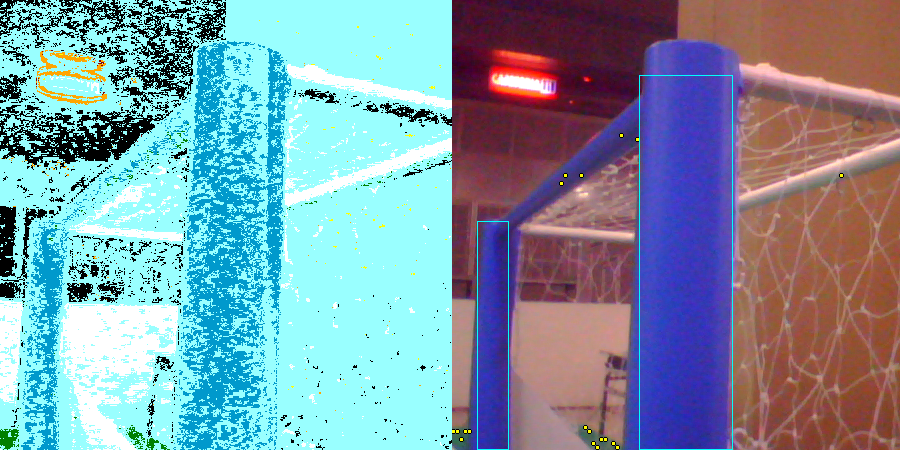
\includegraphics[width=0.7\textwidth]{figures/goalDetection.png}
\caption{A screenshot of the goal detection. The left image shows the colour classified image, while the right image shows the detected goal posts} \label{fig:goalDetection}
\end{figure}

As can be seen in \autoref{fig:goalDetection}, the use of edge detection enables goals to be accurately detected even when a large part of the goal posts has not been classified. 

\subsection{Goal Post Sanity Checks}

With the goal post dimensions now known, a series of sanity checks are used to eliminate false positives. A potential post is considered to be a false positive if:\begin{itemize}
\item{The post is too narrow}
\item{The post is not tall enough. If the bottom or top of the goal post can't been seen (either because it is outside the frame, or a robot is covering the bottom of the post), a much lower threshold is used for the minimum height than when both the top and bottom of the post can be seen}
\item{The post is too wide relative to its height. As with the previous sanity check, a less restrictive threshold is used if either the top or bottom of the post cannot be seen}
\item{The top of the post is below the field edge}
\item{The post touches another post previously identified in the frame. This is to prevent occasional cases where two local maximums are detected in the histogram for one post}
\item{The bottom of the post is above the field edge unless there has been a robot detected directly below the post, as can be seen in \autoref{fig:robotDetection}}
\end{itemize}
%Did not include extra detail on dealing with cases where the goal is on the edge of the image

\subsection{Goal Post Type and Distance Calculation}

A maximum of two posts can be detected in an image. If only one goal post has been identified, the next step is to calculate whether the post is the left post, the right post, or if not enough information is available to determine the type of the post. This is achieved by examining the x axis histogram about the middle x coordinate of the goal post. The histogram is scanned in both directions from this point until a column is reached where no goal coloured pixels were recorded. If one scan proceeds significantly longer than the other direction, this is most likely due to the crossbar, and thus it can be determined if the post found is the left or right post. 

The final stage of the goal detection is to calculate the robot relative coordinates of each post detected. In all cases, the robot relative heading to the post is calculated by using the kinematics chain on the middle of the bottom of the goal post. However, in some cases when the bottom of the post cannot be seen, the bottom most part of the goal passed into the kinematics chain is above the horizon. While this does not affect any distance measurements, it causes the heading to be flipped. Therefore, if the coordinate passed into the kinematics chain is near to the horizon, another pixel well above the horizon is also passed into the kinematic chain and is used for the heading estimate. Note that the exact position of the horizon is not used as inaccuracies and delays in the kinematics chain can cause the heading to be reversed even if the pixel used in the kinematics chain is slightly below the horizon. The robot relative distance is calculated either using the kinematics chain on the middle of the bottom of the goal post or through using the width of the goal post to estimate the distance, depending on what parts of the goal post have been detected. 

If the bottom of the goal post has been detected, the kinematics chain is used for the distance estimates, as the kinematics chain has been found to provide more accurate estimates than the width of the goal posts, as the measurements based on the width are affected by blurring. However, if the bottom of the goal post is not seen, but the left and right of the goal post is inside the image, the width is used for the distance estimate. If a distance estimate has still not been set, the post is not reported as no reasonable distance estimates can be made. When two goal posts are detected in the same frame, the same method for estimating distance is used for both posts.

\section{Camera Colour Space Analysis}
\label{sectionCameraCalibration}

Currently the settings for the Nao's cameras are determined manually through the
use of Telepathe.
During the 2010 campaign we initiated an experiment to auto-calibrate the
camera settings although it was not used during competition and requires further
testing and development.
Essentially, the idea is to adopt settings that would maximise the ``information''
obtained by each camera frame.
One method for achieving this is to calculate the entropy of the image.
This idea has been adopted by  Lu \textit{et al.}~\cite{Lu09} who apply
the following formula:
\begin{equation}
Entropy = - \Sigma_{i = 0}^{i = 255} p_{R_i} log p_{R_i}
          - \Sigma_{i = 0}^{i = 255} p_{G_i} log p_{G_i}
          - \Sigma_{i = 0}^{i = 255} p_{B_i} log p_{B_i}
\end{equation}
where $p_{R_i}$, $p_{G_i}$ and $p_{B_i}$ are the probabilities of each
of the colours in the red, green and blue channels appearing in the image.
In our implementation these probabilities are approximated by the frequency
of occurrence of these colours in each image.

The current implementation of this tab is illustrated in \autoref{figCameraCalibration}.
\begin{figure} [ht]
\centering
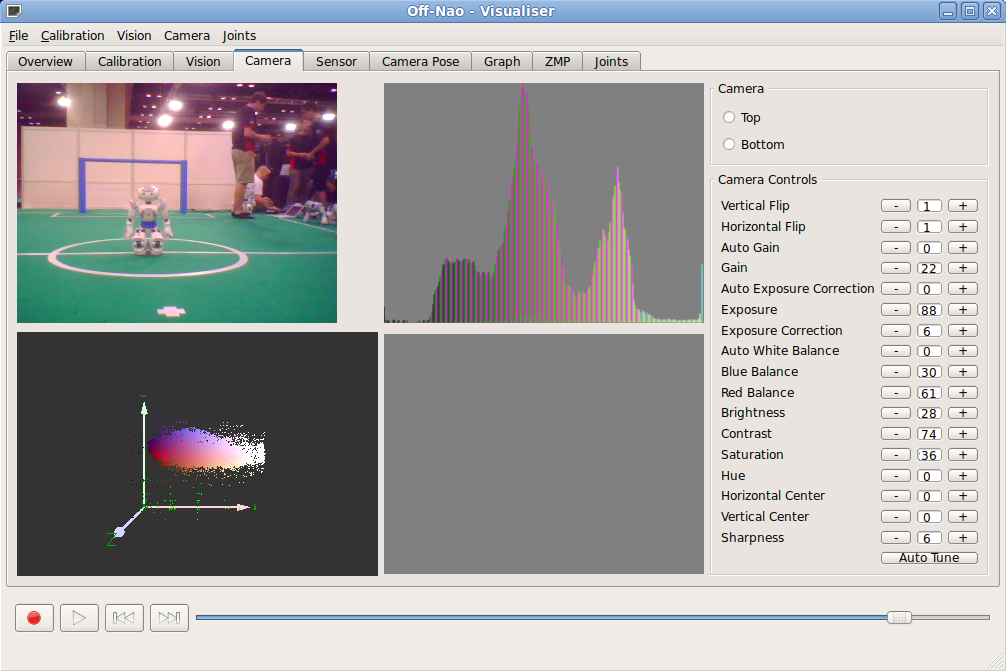
\includegraphics[width=1.0\textwidth]{figures/CameraCalibration.png}
\caption{Camera Calibration Tab.} \label{figCameraCalibration}
\end{figure}
The tab allows for the setting of any individual attribute of the Nao's cameras.
Furthermore, the \texttt{Auto Tune} button implements a hill-climbing
algorithm to determine the best settings.
It is intended to be used by directing the Nao camera towards a scene containing as many
of the colours required for colour classification as possible so that the
camera settings can be calibrated by maximising the entropy (i.e., colour separation)
in this image.

In developing this feature a generic \texttt{Histogram} class was developed so that
the calculations could be performed on a variety of image types.
The current implementation uses the YUV colour space
(whose histogram appears in the top left pane in \autoref{figCameraCalibration})
since it is adopted in the team's code.
However, it can be used with any colour space.
While the technique has been fully implemented it currently only uses the top camera
and has not been empirically tested.
In future work, the current algorithms should be tested to determine their effectiveness.

\section{Results} \label{sectionVisionResults}

While it is difficult to quantitatively evaluate the performance of the vision system, a subjective evaluation of its real world performance on the soccer field is the most important evaluation measure. In this way, the rUNSWift team placed second in the 2010 Robocup competition using this architecture. In particular, it was able to handle the difficult conditions of a final game, where people crowded around the field can pose significant challenges for affecting the lighting and creating false positives, without noticeable degradation in performance. In testing before the competition, we found that vision was able to run at approximately 30 frames per second during game conditions.

As the region builder uses the field edge detection to only scan the image below the field edge, and field edges are used for localisation, field edge detection is a vital part of our vision system. We found that when the field edge(s) could be seen clearly, or with a few small obstructions, the field edge detection worked consistently and accurately. However, when there was a lot of obstruction, such as several robots, or a referee, the field lines were often mis-placed. At times this caused a noticeable deterioration in the localisation while lining up to make a kick for goals. The field edge detection also could occasionally miss the corner of the field when it was near the edge of the image, as not enough of the short field edge is in the frame for it to be found as an edge. These inaccuracies did not noticeably negatively affect the performance of vision. Extra sanity checks were introduced into the ball detection to prevent inaccurate placement of the field lines causing balls to be detected above the field edge.

Throughout the competition, the goal detection performed accurately and consistently, with no major problems observed, and was thus used as the major component of localisation, as can be seen in \autoref{sectionLocalisation}. While goal detection generally had very few false negatives, we found that we had to take care with colour calibration of the goal colours to make sure enough pixels are classified as the goal colour when the robot is on the other side of the field performing a localisation scan. In these circumstances, the goal posts can appear significantly blurred, which can sometimes result in too few goal coloured pixels in the goal post to register a histogram maximum. However, after carefully extending the calibration of the goal colours, we were able to consistently detect goal posts at long distances during head scans. Furthermore, using edge detection instead of colours to determine the exact dimensions of the goals allowed the goals to be detected accurately when the majority of the post was not classified as a goal colour. This was particularly useful for goal detection as the appearance of goals change change quite dramatically depending on the angle and distance they are seen.

Our ball detection also performed accurately and reliably during the competition. The use of edge detection allowed balls to be detected accurately even when the majority of the ball in the image was not classified as orange. A concern we had during the development of the algorithm was that the region builder needs to see at least one orange coloured pixel before a ball can be reported, which could potentially cause distant balls to be missed as the region builder operates only on the saliency scan. However, we found that the saliency scan provided enough resolution to see a ball at the other end of the field during a head scan. During the initial rounds of the competition, we found that the ball detection occasionally reported balls in objects around the edge of the field, such as spectator's leg or shoes, presumably due to slight errors in the placement of the field edge. In order to fix this, we significantly toughened the sanity checks that can remove balls that could potentially not be on the field. This worked very well, and no further false positives around the field edge were noticed. However, this did come at a slight cost of reducing the detection rate of balls across the field. 

One of the major problems we experienced in the weeks leading up to the competition was reporting balls in the red bands of robots. As can be seen in \autoref{sectionBallDetection}, a myriad of sanity checks were introduced to remove this, and during the competition only a few of these false positives were noticed. These mainly happened in unusual situations that the sanity checks weren't designed to handle. For example, balls inside a robot were not deleted if they were at the bottom of the robot region. This was designed as a robot's red band is normally well above the bottom of a robot region, and it not desirable to delete real balls at the feet of robots. However, if a robot has fallen, balls were occasionally reported in the red band. Additionally, false positives were also noticed during the Dribble Challenge, as the robots were squatting low enough for the band to be seen almost at the bottom of the robot region.

Robot detection was the least developed part of our vision infrastructure, and consequently tended to report false positives and false negatives at a significantly higher rate than other components of vision. That said, the robot detection was used unmodified in the Dribble Challenge, in which rUNSWift placed third, helping us to achieve first place in the technical challenges. While in the majority of circumstances the robot detection was able to correctly identify the presence of a  robot and its colour, it was unable to report robots on opposite sides of the field. This was mainly due to the requirement of robot detection to see a minimum number of robot red or robot blue coloured pixels for a robot to be reported. The band of robots a significant distance away from the camera often did not contain enough robot coloured pixels in the saliency scan to meet this requirement. Minimising the number of false positives is the other main area where the robot detection be improved for future tournaments. In order to detect robots whose bands are appear above the field edge in the image, the robot detection scans above the field edge around a potential robot region to see if there are any robot red or robot blue coloured pixels. However, this makes it possible for items in the background to be reported as robots. 

Our field line detection reported the start and send points of scans in regions that were thought to contain field lines. As can be seen in \autoref{sectionFieldLineUpdates}, this was used to localise by matching these points to a precomputed map of the field. The field line detection was successful in providing this information, but, as it only operates on the saliency scan, often field lines on the opposite side of the field were often not reported. However, as mentioned in \autoref{sectionLocalisation}, field line localisation was mainly used for local adjustments of position, missing far away field lines was not a problem. As will be mentioned in \autoref{subsubFutureWorkVision}, we would like to expand the visual processing of field lines for next year's competition to allow global localisation. 

Once an object was found and processing on it finished, the distance to it was
calculated using either the kinematics chain or the size of the object in the
image (for goals and balls only). During testing we found that using the width
of the post or the radius of the ball to estimate distance was generally more
inaccurate than kinematics, as blurring can have a significant affect on the
size of the object. Even so, it was still a useful method to estimate distances
for circumstances where kinematics could not provide a reasonable estimate, such
as when the bottom of a goal post can't be seen. Alternatively, after
calibration, we found that kinematics performed accurately. However, as
expected, the accuracy of kinematics decreases with increasing distance, both
because errors in the precise location of the object in the image and errors in
the joint angle readings have more of an affect as distances away from the robot
increase. 

\section{Future Work} \label{subsubFutureWorkVision}
There are several possibilities for improvement upon the vision system used in the 2010 Robocup competition, including: \begin{itemize}
\item{Multi-resolution processing of the goal posts. Once the maximum histogram points for a goal post are found, the dimensions of the goal post are determined by scanning the full resolution image for edges. When the goals are very close to the camera, this causes the gaol post detection to run slower than is necessary. The magnitude of the maximum in the histograms could be used to estimate the size of the goal posts in the image, allowing different resolutions to be used to find the goal post dimensions.}
\item{Improvements to the robot detection. Improving the rate of false positives and false negatives would allow the development of behaviours that can avoid enemy robots and allow easier passing to friendly robots.}
\item{Use edge detection in more parts of vision. We found that the edge detection used in the ball and the goal detection worked very well, and allowed to keep reliably identifying balls and goal posts in changing lighting conditions. Moving more of our vision code away from colours would further improve this.}
\item{Field line detection could be improved to identify the locations of features, such as the centre circles, corners, and the equations of the actual lines. This would enable field lines to be used for global localisation}
\end{itemize}

\section{Conclusion}

Arguably the most important form of sensory perception, a vision processing system must be highly efficient, robust and accurate to enable it to perform accurately and reliably in the dynamic world of a soccer game. By utilising a hybrid of colour classification and edge detection, we were able to reliably identify robots, goals, field lines and balls during the 2010 Robocup competition. Our approach of using sub-sampled images allowed us to reduce the processing of redundant data, and achieve processing speeds of approximately 30 frames per second, while our use of edge detection allowed the ball and goal detection to perform well in changing lighting conditions.

% **********************************************************************************************************
\newpage
\chapter{Localisation}\label{sectionLocalisation}

\section{Introduction}
Self-localisation is done using a combination of Kalman filter and particle filter. These filters update every cycle based on landmarks perceived in the current image frame as identified by vision. The Kalman filter is good at maintaining a single hypothesis of the robot's location, provided it is given constant updates from various sources. When it does not receive new information or conflicting information over a longer period of time, however, the robot can get lost. It is often difficult to recover from this lost state due to the limited number of visible landmarks available while the robot is, for instance, chasing the ball. The particle filter, however, is good at maintaining multiple hypothesis but requires more intensive calculations as updates have to performed on every hypothesis maintained. Our solution is to take advantage of the Kalman filter's speed and particle filter's accuracy by switching between them intelligently.

\section{Background} 

Developing algorithms that allow a robot to maintain an accurate representation of its state and the state of other interesting objects on the field, such as friendly robots, opposing robots, and the ball, remains one of the most challenging problems in the Robocup Standard Platform League (SPL). The key reason for this difficulty is the lack of accuracy, amount of noise, and sparsity of data in all the robot's sensor observations. With perfectly accurate and continuous vision, odometry, hearing, and timely communication from team-mates, localisation would be simplified to nothing more than performing geometric transformations of observed data into the desired state-space representation. In reality, all these sensors can have very large error margins, completely false observations can be read due to hardware limitations or algorithmic imperfections in the sensory parts of the system, and information allowing the robot to globally localise arrives at infrequent and unpredictable intervals. As a result, in order to maintain some reasonable approximation of the robot's state, filtering techniques must be used. Two particular filtering techniques have emerged as the dominant approaches in SPL: Monte Carlo particle filters, and Kalman filters.

Particle filters are a form of Monte Carlo Localisation \cite{Fox_1999_534} which maintains a set of samples representing the robot's belief state. If the robot knows its position, the samples collapse into a region of concentration on top of the robot's true position. If the robot does not know where it is, then the samples are distributed evenly at all possible positions. At each sensor update, the weights for each particle is updated and renormalised such that they sum to 1. Through either importance (weight) resampling or weight elimination, these samples will eventually collapse into one region, representing the globally localised belief state. The varying sample size leads to non-constant filter run time as each sample needs to be updated every cycle. Compared to uni-modal Kalman filters, particle filters are slow, especially as the state vector grows in dimensionality \cite{rekleitispftut}. However, the samples are capable of approximating almost any probability distribution, which is an advantage when it comes to dealing with non-linear observations and solving the kidnapped robot problem \cite{Burchardt10} --- robots being picked up by referees during game play and placed elsewhere. 

The number of particles required for particle filters often increase exponentially with dimensionality \cite{rekleitispftut}. In the SPL setting, we have 3 dimensions for each robot's position and heading $(x, y, \theta)$. For the ball, there are 4 dimensions $(x, y, \theta, v)$ which are the position, velocity vector heading and speed. This makes up a 22 dimensional vector: 3 robots per team, 6 robots in total on the field, so 18 dimensions for the robots plus 4 for the ball. Given the exponential growth in number of particles, keeping track of all of them on the Nao's hardware is not easily achievable. If the same vector is passed to a Kalman filter, the processing time would remain linear with the number of dimensions, which is one of the big advantages over a particle filter. 

Uni-modal Kalman filters operate by using a Gaussian to approximate the probability distribution of the current state \cite{Welch95anintroduction}. This has the disadvantage of not being able to directly incorporate non-linear observations, but instead requiring that a Gaussian approximation be generated. Kalman filter updates are constant-time, resulting in a significantly reduced processing overhead, but they provide less accurate approximations compared with particle filters. 

In 2006 \cite{olegthesis}, the rUNSWift team devised a hybrid solution, where the state probability distribution is represented by a small number of particles, each of which is a Gaussian. This allowed non-linear observations to be incorporated in a more flexible manner than with uni-modal Kalman filters, whilst maintaining relatively low computational costs. This system was not used by the 2010 rUNSWift team due to the difficulty of producing a robust implementation of this more complex algorithm, however it may provide an appropriate basis for future work in this field.

This year, we propose a system whereby a particle filter is used initially, to produce a location estimate for the robot using early non-linear observations, which, once converged, becomes the starting point for a uni-modal Kalman filter. Observations incorporated into this Kalman filter are linearised using the current state estimate as a basis, allowing rapid updates to the filter. Because non-linear observations can lead to erroneous results with this approach, we track the discrepancy between the Kalman filter's state and new observations, called the \emph{kidnap factor}, and return to the more computationally expensive particle filter when this exceeds a certain threshold. We thereby gain the benefit of the best features of both Monte Carlo Particle Filters and Uni-Modal Kalman Filters, with a reasonably low amortised computational cost.

\section{Kalman Filter Updates}

Each cycle of the Kalman filter, we calculate zero or more hypotheses for the robot's position to update the filter. Most of these hypotheses are generated from a combination of an object detected in the current frame, as well as the current state estimate; others, such as the two-post update, are calculated independently. The standard Kalman filter update function (\autoref{eq:kfup0} \ref{eq:kfup1} \ref{eq:kfup2}) assumes that each update is based on an independent observation, so using data from previous states in producing a hypothesis can create large sampling errors, leaving the filter in an incorrect belief state with a low variance. Repeated updates with the same non-global information causes the variance to tend towards zero, making it increasingly difficult to recover. To solve this problem, we only apply \autoref{eq:kfup2} when there is sufficient information in the camera frame to uniquely position the robot, these are called \emph{global updates}, when only partial information is available, the variance is not updated in what we call \emph{local updates}. The geometric characteristics of each of these updates are described in the following sections:

\begin{equation}
\label{eq:kfup0}
\vec{k} = \begin{pmatrix}
\frac{x_{var}}{x_{var} + x_{obs var}} \\
\frac{y_{var}}{y_{var} + y_{obs var}} \\
\frac{\theta_{var}}{\theta_{var} + \theta_{obs var}} \\
\end{pmatrix}
\end{equation}

\begin{equation}
\label{eq:kfup1}
\vec{S}_t
 =  \vec{S}_{t-1} +
\vec{k} \times
\left( \vec{S}_{obs} - \vec{S}_{t-1} \right)
\end{equation}

\begin{equation}
\label{eq:kfup2}
\vec{var}_t
= (
\begin{pmatrix} 1 \\ 1 \\ 1 \end{pmatrix}
 - \vec{k}) \times
\vec{var}_{t-1}
\end{equation}

\subsection{Local Updates}

\subsubsection{Field-Edge Update} \label{subsubsecFieldEdgeUpdate}

\begin{figure} [ht]
\centering
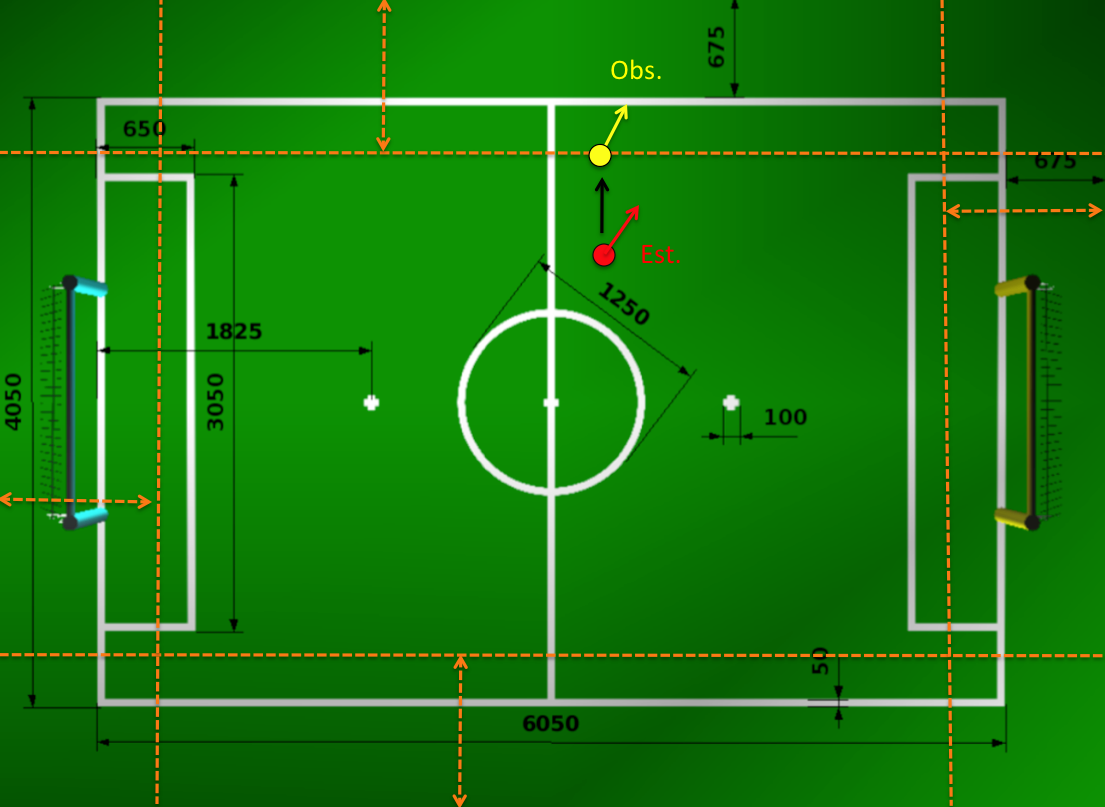
\includegraphics[width=0.8\textwidth]{figures/KFfieldEdgeUpdate}
\caption{Update from field-edge lines, illustrated on the field diagram\cite{RobocupRules}.} \label{figKFfieldEdgeUpdate}
\end{figure}

An innovation made in 2010 by rUNSWift, was to use the field-edges, detected using the technique described in \autoref{secFieldEdgeDetection}, to update the robot's position relative to either the goal line or side line. One field-edge line generates an infinite set of hypotheses (see \autoref{figKFfieldEdgeUpdate}) for where the robot may lie, so we choose the field-edge closest (in terms of orientation) to our current position estimate.

We require the expected orientation of the chosen field edge to be within 45 degrees of the observed orientation to perform an update. If this criteria is met, we then update the orientation and either the x or y (see \autoref{appendixFCS}) position, depending on whether we have chosen a side-line or goal-line.

If two field edges are detected, this procedure is performed iteratively for each one, allowing one good observation to be used even when the other is a false-positive that fails the 45 degrees test.

Because this whole procedure is heavily dependant on the current state estimate, we only perform a local update for field-edge lines.

\subsubsection{Single Post Update}

\begin{figure} [ht]
\centering
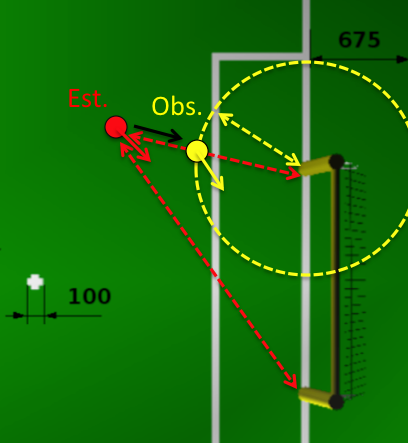
\includegraphics[width=0.8\textwidth]{figures/KFonePostUpdate}
\caption{Update from one goal-post.} \label{figKFonePostUpdate}
\end{figure}

One goal-post generates an infinite set of hypotheses i.e. around a circle radius distance from goal-post center (see \autoref{figKFonePostUpdate}). Furthermore, when we do not know which goal-post we are seeing, such as in frames where the crossbar is not visible, the hypothesis space is two circles. We can perform a local update by using our current estimated position to decide which goal post we are seeing based on a distance measure that takes into account Euclidean distance of $(x, y)$ location and a weighted square measure of angle error to goal post. Then, use a point on the circle of the chosen post closest to our current estimate as the observation fed to the filter.

One drawback of this method, is that we do not take into consideration the co-variance in x, y and theta that a multi-dimensional extended Kalman Filter would.

\subsubsection{Field Line Updates} \label{sectionFieldLineUpdates}

As described in Section \ref{sectionFieldLineDetection}, Localisation has access to a series of robot relative coordinates that correspond to the edge of field lines in the image. These points can be used to determine the likelihood of a robot being in a given position by examining how well the points match a map of the field lines if the robot were in that position.

The map of the field is precomputed and stored as a binary file. It contains a grid of the field at a resolution of 1cm. Each entry in the grid is the distance squared from that point in the field to the closest field line (including the centre circle and penalty spots). A visualisation of this map is shown in \autoref{fig:fieldDistancesMap}. Thanks to Tenindra Abeywickrama for providing this map.

\begin{figure} [t]
\centering
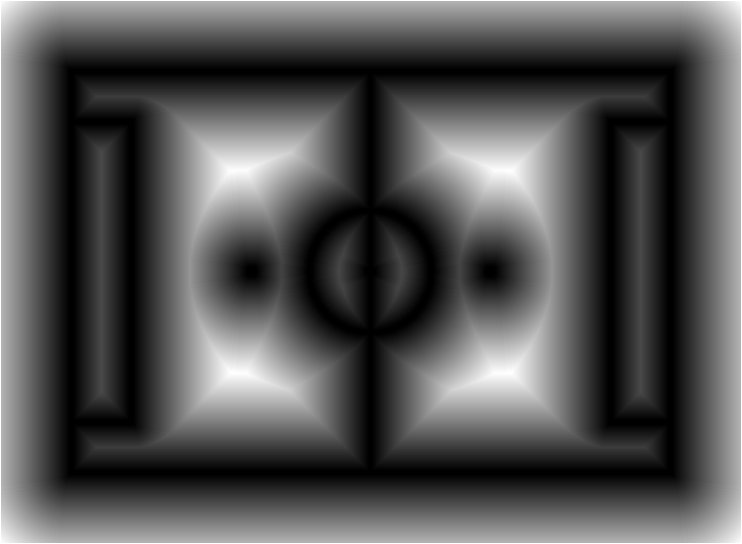
\includegraphics[width=0.7\textwidth]{figures/fieldDistancesMap.png}
\caption{A map of the field line distances, where the lighter the shading, the further away the point is from a field edge} \label{fig:fieldDistancesMap}
\end{figure}

Each time localisation performs a field line update, a telescoping search is performed around the robot's last estimated position to find the best estimate of its current position. At each stage of the search, the likelihood of being in the given position is determined by scanning through the list of field line points, offsetting the points by the position, and determining the entry in the grid that each point corresponds to. The average of each of these entries is taken to be the likelihood of being at that position. 

The telescoping search starts by scanning an area of 20cm each side of the robot at a low resolution, with a variation in the angle of the robot of 5 degrees. A further search is then performed around the position that gave the best position match. The result of this is returned as the most likely position of the robot for the field line update. Examples of good matches using this algorithm are shown in \autoref{fig:fieldLineMatching}. The searches have a small amount of intertia to slightly penalise matches away from the starting position to discourage the returned location drifting when the match is constant along one axis, such as when only one field line is seen. While this search is very efficient, it has the disadvantage of being able to be caught in local minimums.

\begin{figure} [t]
\centering
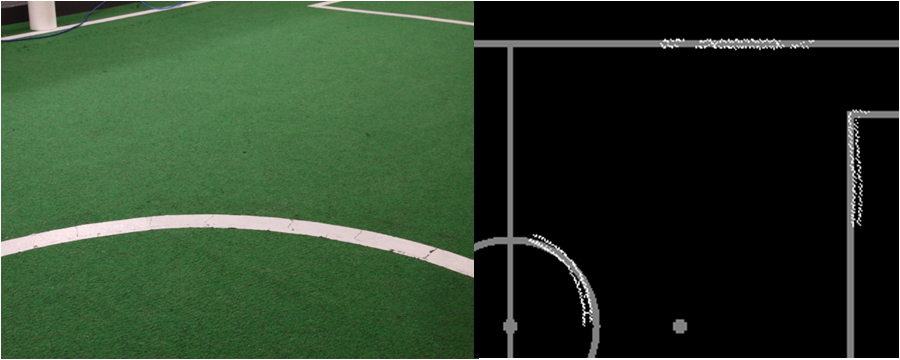
\includegraphics[width=0.7\textwidth]{figures/fieldLineMatching.png}
\caption{An example of a match achieved using the telescoping search} \label{fig:fieldLineMatching}
\end{figure}

\subsection{Global Updates}

\subsubsection{Two-Post Updates} \label{subsubTwoPostUpdates}

\begin{figure} [ht]
\centering
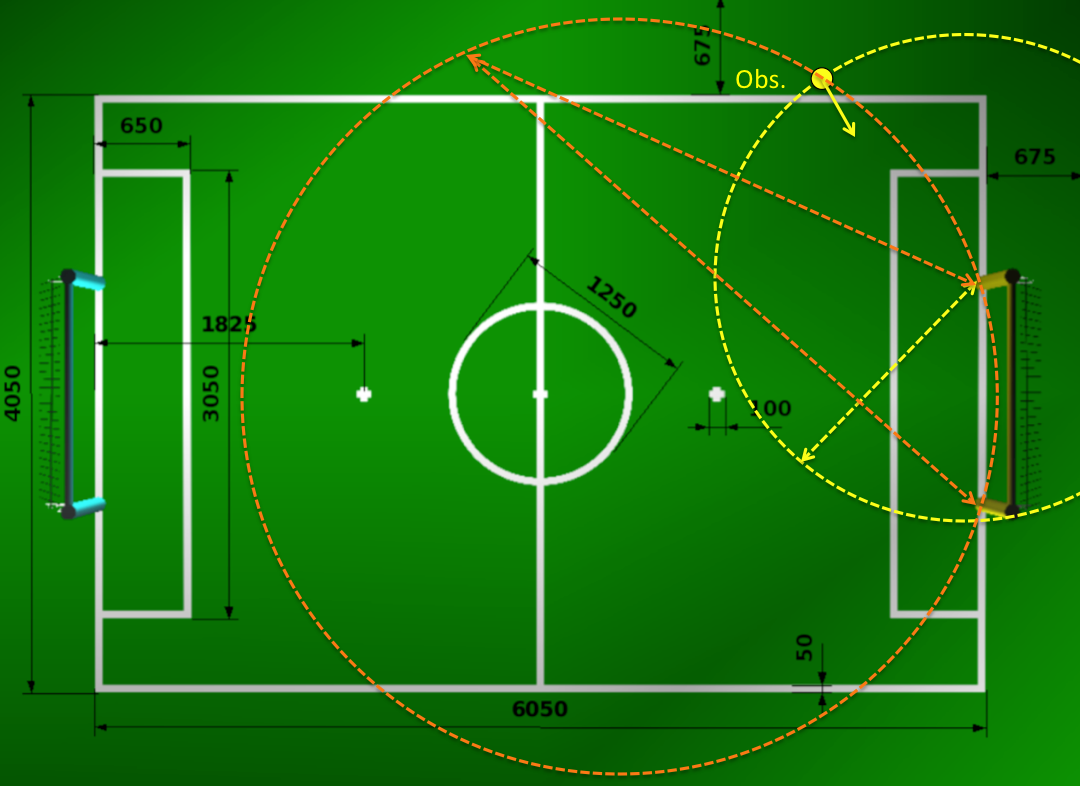
\includegraphics[width=0.8\textwidth]{figures/KFtwoPostUpdateNear}
\caption{Two goal-post update at close range. (Average post distance $<$ 2.5
meters)}
\label{figKFtwoPostUpdateNear}
\end{figure}

\begin{figure} [ht]
\centering
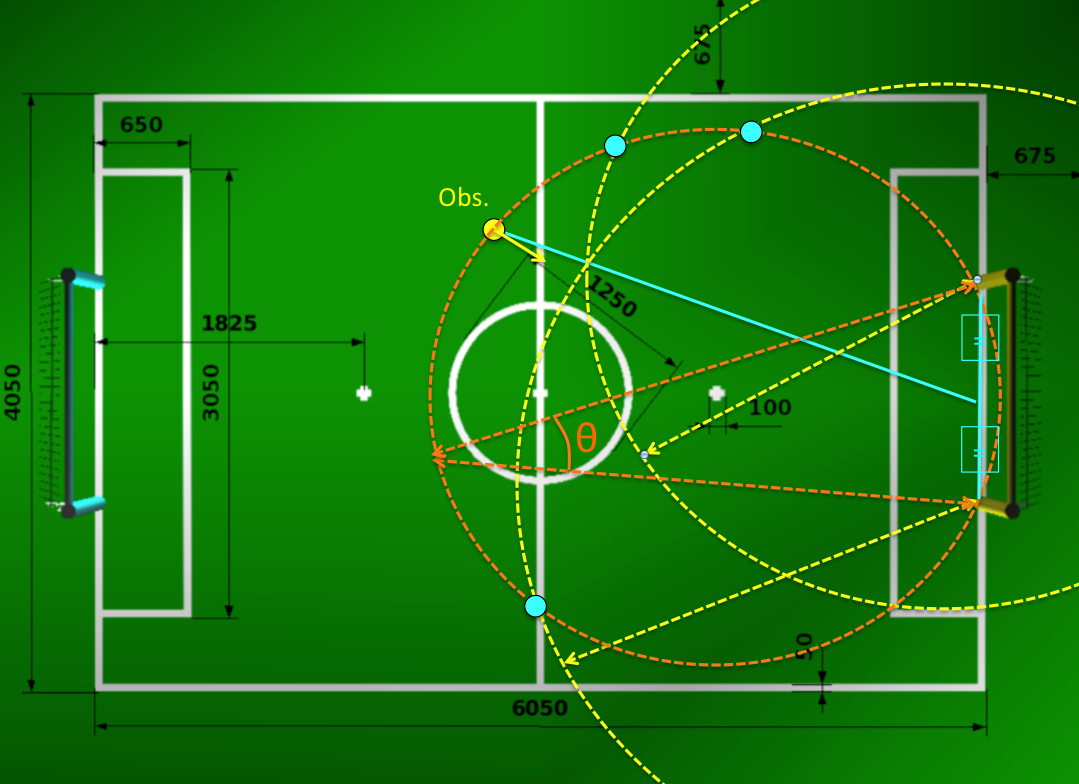
\includegraphics[width=0.8\textwidth]{figures/KFtwoPostUpdateFar}
\caption{Two goal-post update at mid/far range. (Average post distance $>=$
2.5).}
\label{figKFtwoPostUpdateFar}
\end{figure}

In the case that two goal posts are visible, it can provide a single hypothesis
on the field for the robot's location.  As the distances to the goal posts are
generally inaccurate, especially with increasing distance, we have found that
the visible angle $\theta$ between the two goal posts is accurate.  However, the
angle alone does not give us a single hypothesis, but instead a circle of
hypotheses. This is the circle intersecting both goal posts with a radius $r$
such that $2r \sin(\theta) = \textrm{goal width} $ (the orange circle in
\autoref{figKFtwoPostUpdateNear}).

As the distances to the goal posts are somewhat accurate at close distances,
when the robot believes the closer visible goal post is nearby, it uses the
distance to that goal post to create a second circle of hypotheses of the
robot's position. The intersections of this circle and the circle intersecting
the goal posts is used to provide two hypotheses for the robot's position
(the yellow circle in \autoref{figKFtwoPostUpdateNear}). Of the two
intersections, the one that is used is the one that is in-bounds and confirms
that the closer goal post is closer.

At a medium distance to the goal posts, the calculated distances to the goal
posts are not very accurate, but is equally inaccurate for both goal posts'
calculated distances.  In this case, a line projecting from the center of the
goal posts to the point designated by the two goal posts' calculated distances
is used (the blue line in \autoref{figKFtwoPostUpdateFar}).  The intersection of
this line and the circle (orange) intersecting the goal posts is used to
provide two hypotheses for the robot's position.  Of the two intersections, the
one that is used is the one that is in-bounds.

At a far distance, the calculated distances to the goal posts are not very
accurate, and in this case, the distances are barely used.  At this far
distance, the robot's distance from the center line can be approximated using
primarily the circle intersecting the goal posts.  At this distance, we
perform the same calculations as for a medium distance, but we ignore the
width-wide position calculation. (In this case, the width-wise position of the
robot is not affected by the visible goal posts, unless a field-edge is also
seen, as below.)

\subsubsection{Post-Edge Updates} \label{subsubsecPostEdgeUpdate}

\begin{figure} [ht]
\centering
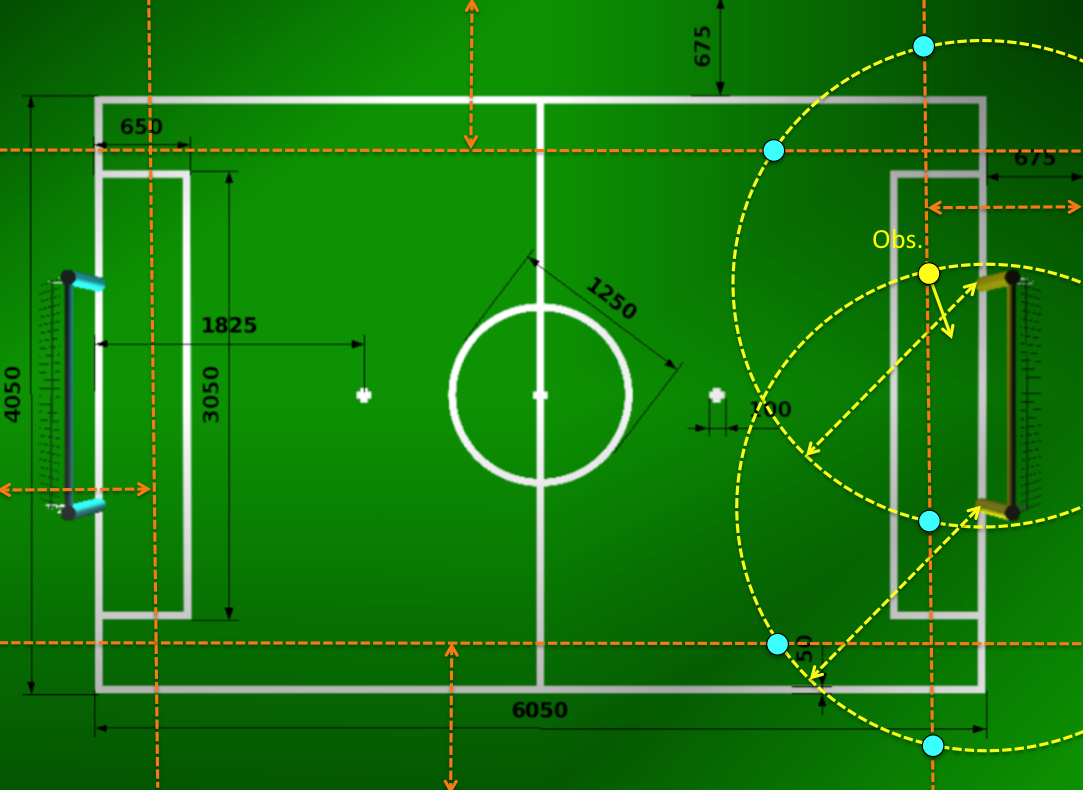
\includegraphics[width=0.8\textwidth]{figures/KFpostEdgeUpdate}
\caption{Observation of position given a field-edge and a goal-post.} \label{figKFpostEdgeUpdate}
\end{figure}

Assuming we are on the playing field, it is possible to generate six hypotheses as shown by the blue and yellow dots in \autoref{figKFpostEdgeUpdate} from a field-line observation and a goal-post observation. The number of hypotheses can be reduced by observing extra field-lines, knowing the identity of the goal-post (left or right), or eliminating ones too far outside the playing area. In this update, we generate all six hypothesis, and then prune them using all information available in the frame. If the number of remaining hypotheses is one, we perform a global update.

\section{False-Positive Exclusion and Kidnap Factor}

A number of methods were used to minimise the impact of false-positives from vision on the accuracy of the Kalman and Particle filters.

\subsection{Outlier Detection Using `Distance-to-Mean'}

If an observation does not correspond with the current belief state by a large margin, it indicates that either the observation is a false-positive, or the current belief state is incorrect by a large margin (i.e. the robot is `kidnapped'). To adequately cope with either situation, we have implemented a feature in our Kalman filter that identifies such anomalies as deals with them:

\begin{lstlisting}
observationError = sqrt(SQUARE(state_vec[i] - obs_state[i])
      / obs_var[i]);
if (observationError > 2.0) {
   outlier = true;
}
kidnapFactor = kidnapFactor*0.9 + observationError*0.1;
\end{lstlisting}

If an observation places the robot a great distance to the current mean belief state, a threshold proportional to the variance of the observation decides if it is an `outlier'. Outliers are not incorporated as local or global updates, and each time an outlier is detected, a value called the `kidnap factor' grows proportional to that error. When the kidnap factor exceeds a certain value, the Kalman filter `gives up' and yields to the particle filter, in the hope of re-starting the Kalman filter from a more accurate state. When only a few outliers are detected, the kidnap factor does not grow quickly enough for the Kalman filter to yield, and those erroneous observations are ignored.

We have found this method provides adequate stability for a single-mode Kalman filter in the SPL tournament, however the need for such methods could be removed entirely by moving to a multi-modal filter that always updates filters only with observations that match the current hypothesis.

\subsection{Intersection of Field Edges and Goal Posts}

A common error case in the Field Edge Detection routine, was the false detection of field edges near the base of the goal post, as it has very similar visual characteristics to an actual field edge, as seen in \vref{fig:EdgeDetection_PostTriangleError}. These field edges were excluded from all filter updates, by requiring a minimum perpendicular distance between detected goal posts and field edges.

\begin{figure} [ht]
\centering
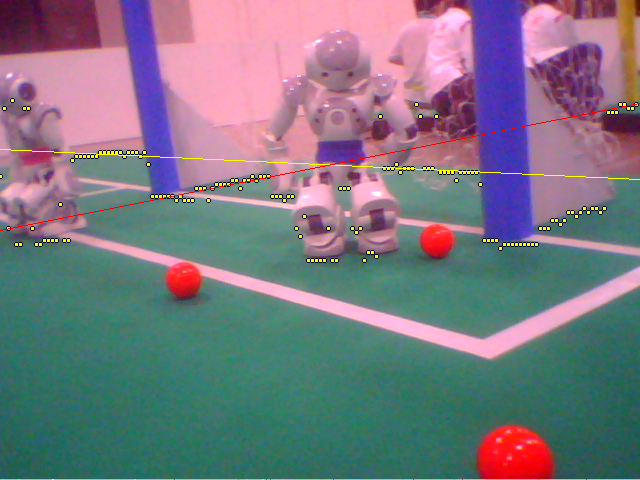
\includegraphics[width=0.7\textwidth]{figures/EdgeDetection_PostTriangleError}
\caption{The red line is a falsely detected field edge, due to the goal post base obscuring the actual field edge} \label{fig:EdgeDetection_PostTriangleError}
\end{figure}

\section{Particle Filter} \label{sectionParticleFilter}

The particle filter is invoked whenever the robot is picked up (as reported by motion via foot sensor values) or the kidnap factor from the kalman filter is sufficiently high, meaning the robot is lost. It then runs in parallel with the kalman filter until it returns a single particle --- a 3--dimensional vector containing the robot's absolute position and heading $(x, y, \theta)$, which the Kalman filter adopts. 

A simpler variant of the particle filter is implemented without resampling \cite{probablisticRobotics} aimed at reducing processing time. Particles are eliminated on the basis on weights, which measures the likelihood of the observation being made from the give position. This means particles start with weights of 1 initially, and at each observation the previous weight is multiplied with the current weight. One side effect is the weights of particles close to the true position can end up being very low, e.g. if there is an outlier in the observation, and are eliminated early. To compensate for this, weights are renormalised after each filter cycle and a higher resolution of particle distribution is required to desensitise the filter to noise in observations.

Given the relatively high frame rate (about 30 frames per second) from vision and the short expected run time of the filter, we make the assumption that particles generated remain in fixed positions. No new particles are generated unless the filter discards all current ones at once.

In addition to weight elimination, the filter also uses a bounding box criteria (see \autoref{subsecBoundingBox}) for collapsing particles. Due to the noise in observations from vision, field edges obtained from vision are first sanitised to throw out invalid edge lines e.g. seeing two non-intersecting field edges in the same frame. 

\subsection{Filter Process}
The filter process is summarised in \autoref{figParticleFilterProcess}.
\begin{figure} [ht]
\centering
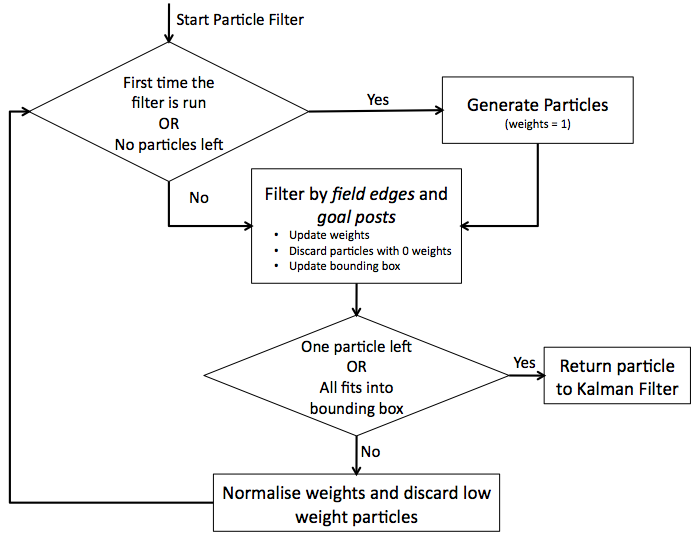
\includegraphics[width=1.0\textwidth]{figures/ParticleFilterProcess.png}
\caption{Particle Filter Process Summary.} \label{figParticleFilterProcess}
\end{figure}


\subsection{Weight Updates} \label{subsecWeightUpdates}
Every cycle the filter is run, particles' have their weights updated based on the latest set of observations made. These Gaussian weights are then used to determine if a particle should be discarded. Each dimension of the particle has a weight, they are updated as follows: 
\begin{equation}
  \begin{pmatrix}
    w_x \\
    w_y \\
    w_\theta
  \end{pmatrix}_t
  =
  \begin{pmatrix}
    w_x \\
    w_y \\
    w_\theta
  \end{pmatrix}_{t-1}
  \times
  \begin{pmatrix}
    g_x &=& g(o_x, \mu_x, v_x)\\
    g_y &=& g_x \\
    g_\theta &=& g(o_\theta, \mu_\theta, v_\theta)
  \end{pmatrix}
\end{equation}
where
\begin{itemize}
  \item $\mathbf{o}$ is the observed distance/heading to the landmark given by vision, e.g. a goal post
  \item $\mathbf{\mu}$ is the theoretical distance/heading to the landmark for the particle we are calculating the weights for
  \item $\mathbf{v}$ is the observation variance for the given dimension i.e. $x$, $y$, or $\theta$
  \item
\begin{equation}
  g(x, \mu, \sigma^2) = \frac{1}{2\pi\sigma^2}\exp^{\frac{-(x - \mu)^2}{2\sigma^2}} \\
\end{equation}
\end{itemize}
Note: 
\begin{itemize}
  \item All particles start with weight 1 when they are first generated.
  \item The weights for $x$ and $y$ are identical, since we do not have a proper covariance matrix and in fact, vision returns the same variance for its $x$ and $y$ observations. 
\end{itemize}

To avoid comparing particles by weight dimension-wise, we compress the weight vector into a single number (referred to as weight from now on):
\begin{equation}
  weight_p = 0.35weight_x + 0.35weight_y + 0.3weight_\theta
\end{equation}
This formula is designed to bias towards position accuracy over heading for fast collapse to the correct position, rather than having to slowly throw out particles of correct heading but different in position.

\subsection{Discarding Particles}

Once all particles have their weights updated, they are normalised to give a sum of one for each dimension. The filter will then discard any which falls below a dynamic threshold. Let $p_0$ be the particle with the highest weight, we can calculate the threshold using the 3 component weights of $p_0$:   
\begin{equation}
  limit_w = \frac{min(weight_x, weight_y, weight_\theta)}{\textit{number of particles}}
\end{equation}

\subsection{Particle Generation}

Particles are generated when the filter is first invoked or when all particles are eliminated after the last observation. All generated particles have weight of 1.

Observations from vision are ranked in order of priority, only the highest priority observation is used to generate hypothesis and the resulting particles will be processed with the aid of other lower order observations if needed:
\begin{enumerate}
  \item Two goal posts --- due to the limited field of view on the robot, this means either two yellow or two blue goal posts. Only one particle will be generated from this case as the Kalman filter would.
  \item Two field edges --- this produces 4 particles corresponding to each of the four corners of the field. Since an edge is a parameterised line given in robot relative coordinates, we can calculate the distance $d_{edge}$ to each edge geometrically by calculating the $x$ and $y$ intercepts for each line (see \autoref{figFieldEdgeCalc}). Then subtract them from each of the absolute coordinate of the corner. Similarly, the absolute heading of the particle can be found by calculating the enclosing angle $\theta_{edge}$ between the robot's x-axis and the edge, then add on to the orientation of the edge.
\begin{figure} [ht]
\centering
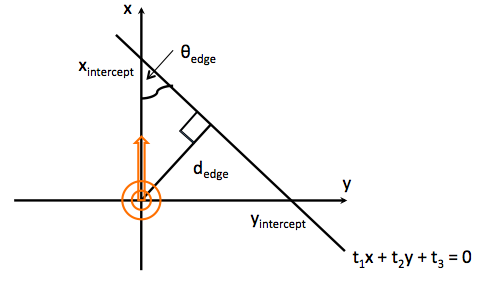
\includegraphics[width=0.7\textwidth]{figures/EdgeCalculations.png}
\caption{Working with field edges: the eccentric circles denote the robot's position, and the hollow arrow denotes the robot's heading.} \label{figFieldEdgeCalc}
\end{figure}


  \item One goal post --- vision reports a post of a known colour with a robot relative distance and heading. However, it may report a goal post with a known left/right placement e.g. BLUE\_LEFT, or of ambiguous placement e.g. BLUE\_EITHER.
    \begin{itemize}
      \item Known placement --- this produces at most 36 particles with a step size of 10 degrees, forming a circle around the given post. This is often not a full circle, since the robot cannot be off the field during game play.
      \item Unknown placement --- similar to the known placement, we generate two sets of particles one for left post and one for the right post.
    \end{itemize}
    These particles will then be filtered using any single field edges seen (if any).
  \item One field edge --- there are 4 edges along the field, a draw back of the current filter is that it does not correlate with prior observations explicitly. Hence, all 4 possible edges are considered, each providing particles end-to-end with a step size of 200mm. Using this step size, no more than 110 particles will be generated given the current field dimension. The particles will form a line parallel to the edge by subtracting the edge's distance (calculable as discussed for the two edges case above) from the coordinates at every step on the edge. Either $x$ or $y$ is updated from the edge distance, and the one dimension not calculated from the distance takes the value dictated by the current step count along the edge. Similarly, the robot's heading is calculated once for each edge, since the particles are parallel to the edge. Visually these particles form a rectangle on the field, each side are of the same distance to the actual field edge.
\end{enumerate}

 \subsection{Filter by Posts and Edges}
 \begin{itemize}
   \item[\emph{Field Edges}] For each particle, work out whether the side-edge or goal-edge is visible as in the Kalman filter (see \autoref{subsubsecFieldEdgeUpdate}). The robot's relative distance and heading of the edge is calculated as per normal, these will then be used to update the weights as described in \autoref{subsecWeightUpdates}.
    \item[\emph{Two Goal Posts}] This simply calculates a single particle as the Kalman filter would, hence no further weight updates are carried out.
    \item[\emph{One Known Post}] For each particle in the filter, we calculate the robot relative distance and heading of the post using their absolute coordinates. These are then used to update the particle's weight as described in \autoref{subsecWeightUpdates}.
    \item[\emph{One Unknown Post}] Same as for one known post, except it will provide two weight updates one for the left post and the one for the right. The filter uses the higher weight of the two for the particle.
\end{itemize}
If the current observation is not possible from the given particle, in other words, we cannot calculate the necessary robot relative distance and heading information; the particle's weights will not be updated (referred to as ``0 weights'' in \autoref{figParticleFilterProcess}) and it will be discarded immediately. For example, the observation includes a field edge, but it is impossible for the robot to see an edge at the given distance away from the particle. 

 \subsection{Bounding Box Criteria} \label{subsecBoundingBox}
 To speed up the collapse of the particles and in the absence of a sophisticated particle distribution detection system, we use a simple ``bounding box'' --- the largest $(x, y)$ coordinate and the smallest $(x, y)$ coordinate. It is reset at the start of each filter cycle to the smallest and largest integer values respectively. If the weight for a particle is updated successfully, the bounds of the bounding box will be adjusted to include this particle if not so already. After all the filtering is complete (i.e. all the weights has been updated), the bounding box is checking by calculating the distance between the two points (i.e. largest and smallest coordinate), if they are less than 600mm, the list of particles is reduced to the one with the highest weight. In other words, the particle filter is ready to stop and pass its results to the kalman filter.
 
\section{Ball Filter} \label{secBallFilter}

To meet behavioural needs in varying situations, such as when the ball is seen directly, the ball has not been seen for some time, and the ball has been seen by a team-mate directly, rUNSWift 2010 maintained three separate Kalman filters, described in the following sections:

\subsection{Robot-Relative Ball Position}

The simplest of the ball filters, which we call the `RR' filter, is simply updated at a fixed, hand-tuned learning rate of 0.6, for each raw visual observations of the ball. The state of this filter is stored as distance and heading from the robot observing the ball. The filter also maintains how many frames it has been since the ball was last seen, to give behaviour an indication of the reliability and accuracy of this data.

This is the filter that was used when attempting to do careful close-quarter work with the ball, such as dribbling or lining up to kick.

\subsection{Egocentric Absolute Ball Position}

The `Ego' filter transforms a ball observation into field-coordinate space (see \autoref{appendixFCS} using the current state estimate from localisation, before applying this position estimate to the filter. The sum of the observation variance and the robot's position variance are used as the observation variance when making an update.

This filter was found to be unhelpful for tasks such as lining up to kick the ball, because of the large errors introduced in the ball position when the robot's position is updated by new localisation data. It was, however, useful for positioning a supporter on the field relative to the ball, as it simplified calculations performed in field-coordinate space.

The current state of this filter was transmitted to all other robots on the team at a rate of 5Hz.

\subsection{Team Shared Absolute Ball Position}

The final filter used was the `Team' filter. Each iteration of the team filter uses the current robot's Ego filter state as a starting point, and updates the filter once witch each of the other robot's Ego ball filter states. This allows a robot who may not have seen the ball for some time, such as a robot stranded at the other end of the field, or one who has recently returned from penalty, to gain an inkling for where the ball may be, and start searching in that region in the hope of updating its own RR and Ego filters.

\section{Obstacle Filter}

To enable the development of behaviours for the `Obstacle Challenge' in the 2010 SPL tournament, it was necessary to provide behaviour with information about where obstacles are currently believed to be. Two approaches were developed in parallel, one using a multi-modal Kalman filter, the other using an adaptive fixed-particle filter.

\subsection{Multi-modal Kalman filter}

Each hypothesis tracked by the filter is represented using the following data structure:

\begin{lstlisting}
struct RobotObstacle {
   RRCoord pos;    // location of the obstacle relative to the robot
   int lostCount;  // num frames since the obstacle was last seen
   int seenCount;  // num times the obstacle has been seen
   RobotType type; // type of obstacle {red,blue,unknown}
}
\end{lstlisting}

In each perception cycle, all currently tracked obstacles' positions are updated according to the robot's odometry, their process variance is applied, and their {\tt lostCount} is incremented. Then, obstacles whose {\tt lostCount} exceeds a certain threshold are discarded.

Any new observations found in the current vision frame are then processed, by updating the filter for the closest matching currently tracked obstacle, or creating a new {\tt RobotObstacle} if none match within a certain threshold.

\subsection{Adaptive Fixed-Particle Filter}

Probabilities were assigned to particular locations on the field using observed data. These probabilities partially moved with the robot (to account for localisation mis-prediction), and partially stayed fixed in the field --- this meant that even if the robot's localisation was jumping about the place, a sufficiently large obstacle would still be detected, particularly if it had been `seen' by multiple robots.

\begin{figure} [ht]
\centering
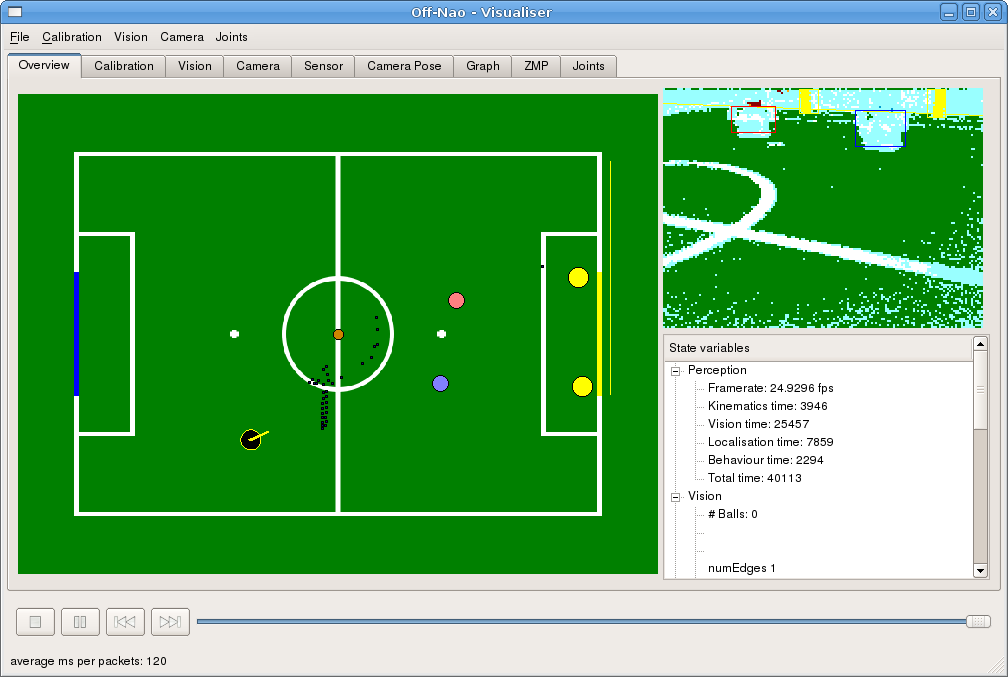
\includegraphics[width=1.0\textwidth]{figures/obstacleFilter}
\caption{The blue and pink dots shown in Off-Nao are robot obstacles being tracked by the filter} \label{fig-obstacles}
\end{figure}

\section{Discussion}

The localisation system developed in 2010 experienced a myriad of problems during development. In game-play, our localisation subsystem would not infrequently report a position that is more than 1 meter away from the true ground position, making the data provided unsuitable for blind use by behaviour. We are still a long way from the goal of \emph{passively} localising whilst focusing on playing soccer, all behaviours had to be tuned for the expected differences in position variance depending on what features are being looked at. Behaviour would perform certain head scan routines before lining up to shoot a goal to maximise the probability of being correctly localised.

The biggest difficulty was that whenever the localisation system was adjusted or re-tuned, the numeric constants used in behaviour would no longer  be useful, and would have to be re-tuned. As a result of this ongoing problem, we stopped development on localisation except for critical bug fixes a month before the competition in Singapore.

Another difficulty encountered was with the speed differences between the Kalman filter and the particle filter. Behaviours that rely on a fixed number of perception cycles can not predict when the particle filter will be entered, and may be unreliable. This was mitigated to a great extend by using timers instead of cycle counters.

Switch to the particle filter proved to be very useful, especially when the robot was stuck in a situation where no global information could be gleaned in any single frame. The speed of the Kalman filter allowed the processor to be utilised by Vision most of the time, helping reach towards the desired 30 fps frame-rate.

Overall, this year's system, whilst not the most accurate to be found at Robocup 2010, provided a reasonable trade-off between performance and simplicity, and was sufficient for most of our behaviours to perform reasonably well.

\section{Future Work}
For 2010, we have a implemented a fast but less sophisticated localisation system. There are several possible improvements to this system, including:
\begin{itemize}
  \item \emph{Better field line localisation} --- Landmark based field line localisation (relies on vision, see \autoref{subsubFutureWorkVision}) such that, we can actually generate hypotheses and update weights from the field lines in view for the particle filter. For the Kalman filter, this also gives us an edge over the other teams since the robots no longer need to constantly look up to localise off goal posts and distant field edges, instead they can track the ball and still maintain a localised state with the aid of the field lines. 
  \item \emph{Kalman filter sharing its hypothesis with the particle filter} --- Our Kalman filter implementation occasionally generates a set of hypotheses for its updates. For example, when the robot sees a single post and an edge (see \autoref{subsubsecPostEdgeUpdate}). If at this point, the kidnap factor of the robot exceeds the threshold and the particle filter is invoked, it will be of great benefit for these hypotheses being consider first. The particle filter would likely return a probable position for the robot within a few frames, reducing the run time of the computationally expensive filter.  
  \item \emph{Distributed, multi-modal, unscented, Kalman/particle filter hybrid} --- Different combinations of Kalman and particle filter model hybrids as we have here, but more sophisticated models which gives us better accuracy and speed overall. Or perhaps, simply use one type of filter and use it well. 
  \item \emph{Include distributed ball motion model in unified world model} --- This allows all the robots to have share a global ball position with enough accuracy to enable gameplay e.g. kicking, ball intercept planning, passing, and so on. The ball model should also include a velocity component $(\theta_{ball}, v_{ball})$ such that, the robots can predict the future position of the ball, which enables a more sophisticated and dynamic team play to be developed. 
  \item \emph{Include robot positions into unified world model} --- Having robots knowing with confidence their team mates' positions and opposing robots' locations, allows for better behaviour and team play. This may require other types of sensors to be used, such as sound and sonar, together with a more robust form of visual robot detection.
\end{itemize}

\section{Conclusion}
Localisation is a key component in the overall system architecture. This year, we implemented a hybrid model of uni-modal Kalman filter running in conjunction with a non-resampling particle filter. With a number of innovative ideas including: localising off field edges, performing updates from field lines and incorporate a mesh of local and global updates accordingly. These allowed our localisation system to perform with speed whilst still maintain a degree of accuracy suitable for game play. This in turn enabled other key components, namely vision and motion, sufficient processing power to perform their roles and keep the system as a whole performing well. The current localisation infrastructure, together with lessons learnt, should provide a good starting point for future teams.
	
% **********************************************************************************************************
\newpage
\chapter{Motion and Sensors}
\section{Introduction}\label{sectionMotion}
Humans are fascinated by robots that mimic their form and movement. It is not surprising therefore that scientists and engineers are researching and developing  humanoid robotic motion. The motivation, and some argue rationalisation, is that robotic assistants in a human form allow for more natural man-machine interaction and avoid the need to modify our environment and tools to accommodate them.  

When we think of humanoid motion, bipedal walking comes to mind. While there is a considerable body of work on this subject, humanoid motion also includes running, dancing, kicking, lifting, balancing, reaching, grasping, manipulating, carrying, driving and bike-riding. The challenge of programming a humanoid robot to perform all of these motions purposefully and gracefully is still an open research problem, although there are many impressive examples of specialised behaviours.

The research and development of bipedal motion addressed in this report is concerned with the ability of a small humanoid robots to play soccer. Soccer requires rapidly changing omni-directional locomotion and kicking abilities. Our demonstrator is the 2010 Robocup Standard Platform League competition using the Nao robot \cite{aldebaran10developer}. Clearly fast locomotion affords an advantage, but speed needs to be counterbalanced by other considerations such as: the robot's physical abilities; energy usage and overheating problems; and staying balanced on two feet while changing speed and direction in the cut and thrust of a soccer match. 

We experimented with several walk and kick types, some of which in the end were not competitive. Our philosophy was not to prejudge the usefulness  of any of the walks and kicks, but leave team members free to choose which actions they wanted to use to write skills and behaviours to achieve specific objectives. For the competition we chose to use a combination of the manufactures supplied walk and a version of our own \emph{Fastwalk} we named \emph{Patter}. For kicking we settled on kicks evolved from an earlier walk called Slowwalk.  

The rest of this report will give a brief background on bipedal locomotion and related work, followed by the motion architecture on the Nao and a detailed description and analysis of the various walk styles and kicks that we investigated. 

\section{Background} 
\subsection{Walk Basics}\label{sectionWalkBasics}

\begin{figure}[ht]
  \centering
  \begin{minipage}[b]{8 cm}
    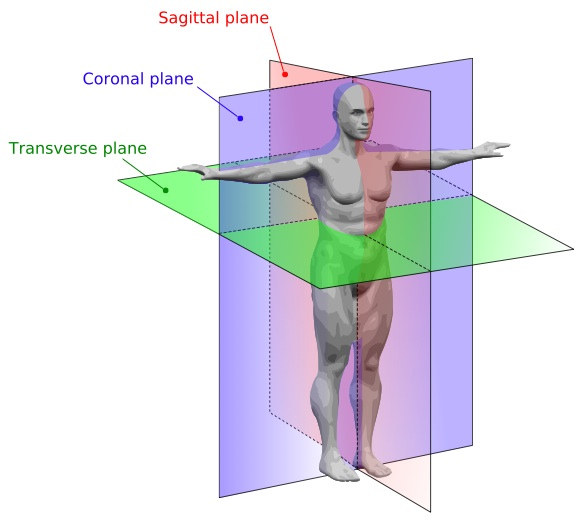
\includegraphics[width=0.8\textwidth]{figures/BodyPlanes.jpg}  
  \end{minipage}
  \begin{minipage}[b]{8 cm}
    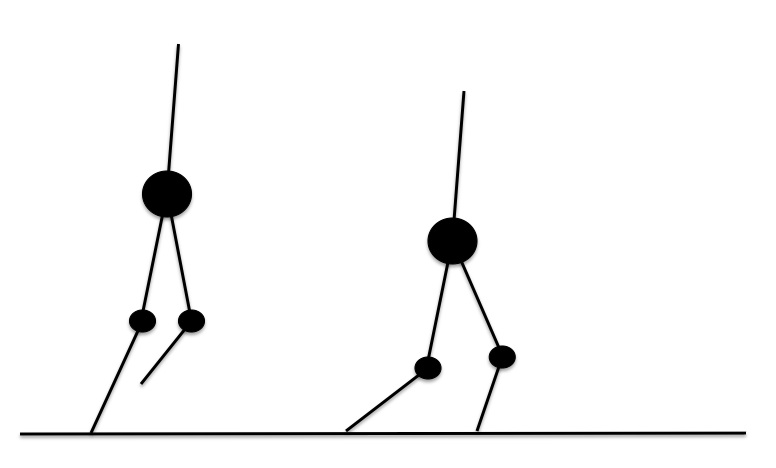
\includegraphics[width=0.8\textwidth]{figures/SingleDouble.jpg}  
  \end{minipage}
  \caption{Human Body Planes (left). Single and Double Support Walk Phase (right).}
  \label{figWalkBasics1}
\end{figure}

A biped is an open kinematic chain consisting of at least two subchains called \emph{legs} and often a subchain called the \emph{torso}. Additional subchains for a humanoid robot include \emph{arms} and a \emph{head}. One or both legs may be in contact with the ground. The leg in contact with the ground is called the \emph{stance} leg in contrast to a \emph{swing} leg \cite{Westervelt:2007fk}. One complete cycle of a bipedal walk can be partitioned into two phases, one per leg. There are two types of partition: a stance phase, followed by a swing phase; or a single support phase followed by a double support phase --- see \autoref{figWalkBasics1} (right) \autoref{figWalkPhases}. The three orthogonal human body planes (sagittal, coronal and transverse) are shown in \autoref{figWalkBasics1} (left).

\begin{figure} [ht]
\centering
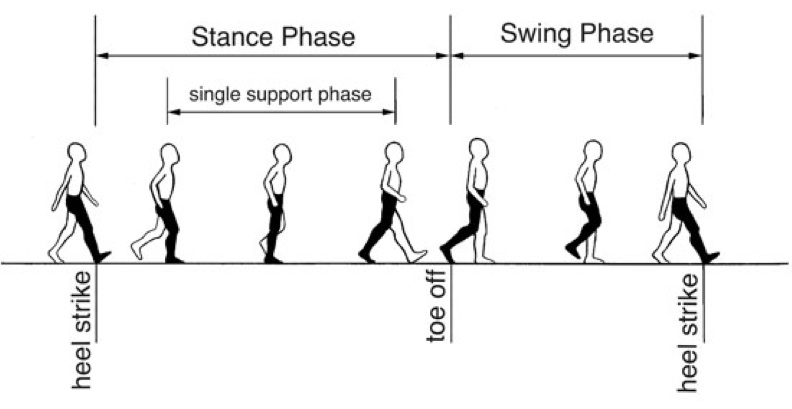
\includegraphics[width=0.8\textwidth]{figures/WalkPhases.jpg}
\caption{A complete walk cycle showing the stance and swing phase of the right leg in the sagittal plane \cite{harrington05symptoms}.} \label{figWalkPhases}
\end{figure}

The center of pressure (CoP) is the point on a body where the total sum of the pressure field acts, causing a force and no moment about that point. The \emph{Zero Moment Point} is defined as that point on the ground at which the net moment of the inertial forces and the gravity forces has no component along the horizontal axes. When the body is dynamically balanced the ZMP and the center of pressure (CoP) coincide. For an unbalanced body, the CoP is at the edge of the support polygon and the ZMP does not exist (or is a fictitious value outside the support polygon) \cite{DBLP:journals/ijhr/VukobratovicB04}. \autoref{figZMP} shows ground reaction forces acting on a stance foot and an equation for calculating the CoP (and ZMP) $p$. 

\begin{figure} [ht]
\centering
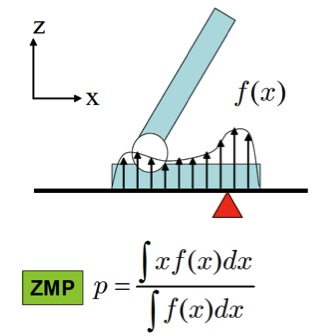
\includegraphics[width=0.4\textwidth]{figures/ZMP.jpg}
\caption{Center of Pressure and Zero Moment Point for a dynamically balanced foot.} \label{figZMP}
\end{figure}

\subsection{Related Work}

There is a considerable and growing body of literature on robotic  locomotion including bipedalism. Advanced humanoid robots include Honda's Asimo, Sony's Qrio, Toyota's humanoid and the HRP range at AIST. Many of these robots use the ZMP concepts originally developed by Vukobratovic and Stepanenco in 1972 \cite{DBLP:journals/ijhr/VukobratovicB04}. Reactive feedback control can be inadequate to balance a humanoid and successful application of ZMP control relies on anticipating the next step and taking control action even before the stance leg leaves the ground. This type of feed-forward control has been called preview control \cite{Kajita03bipedwalking}. Much of the research on bipedal locomotion relies on variations of an inverted pendulum model. The three link system in \cite{feng08biped}, for example, includes a point mass in each of the legs. 

The Standard Platform League originally used the Sony AIBO robotic quadruped. The league took a significant step forward in 2000 when the University of New South Wales developed a competitive walk that later became the standard for the competition \cite{DBLP:conf/robocup/HengstIPS01}. With the introduction of the Nao robots three years ago, bipedal walking became the new challenge.  

In 2009 several universities had developed their own walks for the Nao. The University of Leipzig's Nao-team HTWK used evolutionary algorithms to optimise a closed-loop walk with a reported maximum speed of 32 cm per second in the forward direction. The low vertical actuation of the legs would often cause the robot to fall over \cite{htwk09teamreport}. The Northern Bites team from Bowdoin College implemented an omni-directional ZMP feedback based walk that achieved a stable maximum forward walking speed of 10.5 cm per second. One notable aspect of this walk is the use of efficient iterative inverse kinematics for foot placement \cite{DBLP:conf/robocup/StromSC09}. Their implementation uses \emph{Mathematica} to produce symbolic equations to perform the forward kinematic transforms and final desired joint movements. While we implemented closed form inverse-kinematic equations for walking forward and sideways, we largely relied on this technique in 2010 for turning movements because of the complexity of the hip joint of the Nao. 

Dortmund University of Technology developed a closed-loop walk based on ZMP control \cite{Czarnetzki10applying}. Their ``observer-based'' controller included integral tracking error, proportional state feedback and ZMP preview components. This walk was reported to be stable to external disturbances and able to walk on inclined planes tilted at 6 degrees from horizontal. 

University of Bremen's team B-Human have generated exemplary motions for the Nao \cite{thomas09code}. The inverse kinematic transforms are in closed-form made possible  given the constraints on the Nao's kinematic chains. The walk is closed-loop and balanced by modifying the positing of the next step. The parameter settings of the walk are optimised using a particle swarm algorithm. A smooth transition between different motions is achieved by interpolation. 

In 2009 Tay developed rUNSWift's first bipedal walk \cite{aaron10walking} for the Nao robot. While Tay's omni-directional open-loop walk was faster then the manufacturer's supplied walk at the time, it could become unstable. Without feedback the robot would fall over. This year we redeveloped omni-directional locomotion for the Nao using closed-loop control in both the coronal and sagittal planes. The new walk was competitive in practice on the real robot in the 2010 competition. A detail description of the walk follows in \autoref{sectionFastwalk}. 

Research in the AI Group, CSE, UNSW includes applications of Machine Learning to bipedal gaits. Yik (a member of the champion 2001 four-legged team) collaborated with Gordon Wyeth of the University of Queensland to evolve a walk for the GuRoo robot \cite{wyeth03evolving}, which was entered in the humanoid robot league. This method was inspired by the gait learning devised for the Aibos by Kim and Uther \cite{Kim03automaticgait}. For the humanoid, the same philosophy is applied. Starting from a parameterised gait, an optimisation algorithm searches for a set of parameter values that satisfies the optimisation criteria. In this case, the search was performed by a genetic algorithm in simulation. When a solution was found, it was transferred to the real robot, working successfully. Subsequently, the approach we used was a hybrid of a planner to suggest a plausible sequence of actions and a numerical optimisation algorithm to tune the action parameters. Thus, the qualitative reasoning of the planner provides constraints on the trial-and-error learning, reducing the number of trials required \cite{yik07locomotion} \cite{DBLP:series/sci/SammutY10}

\section{Motion Architecture}
\begin{figure}[ht]
    \begin{center}
        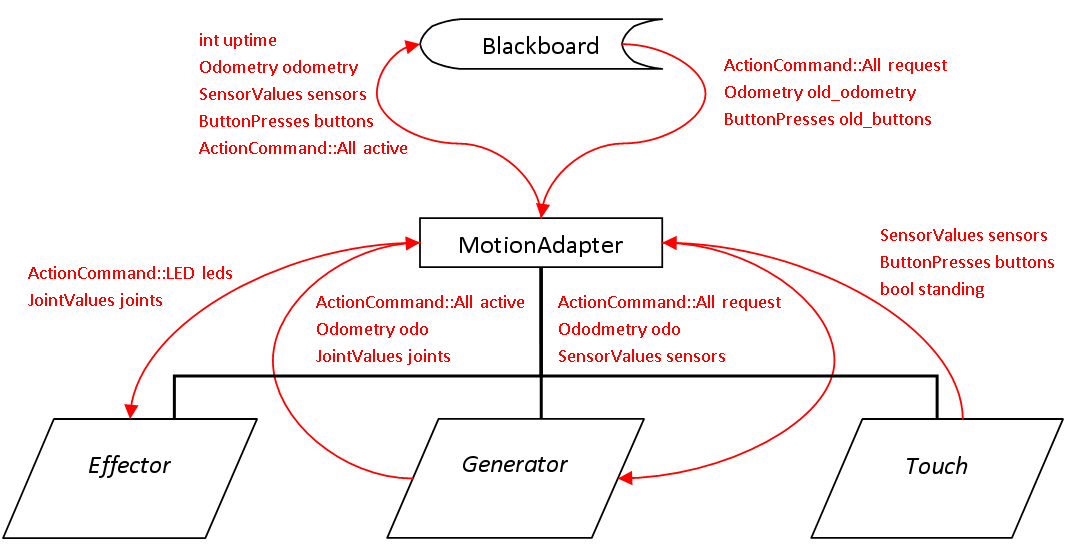
\includegraphics[width=\textwidth]{figures/motion_arch}
    \end{center}
    \caption{The motion architecture. \emph{Red} indicates data flow;
    \emph{black} indicates ownership.}
    \label{fig:motionArch}
\end{figure}

The motion architecture is built on-top of a real-time thread that runs
with higher priority than anything else on the robot. This is needed as
joint angles need to be calculated every 10 milliseconds, or else the robot
will become unstable. This also means that our normal debugging framework
cannot be used within motion, as it might block while writing to the log
file.

Overall control of the Motion thread is provided by the
\emph{MotionAdapter} class. The MotionAdapter in turn owns a
\emph{Touch} object, a \emph{Generator} object and an \emph{Effector}
object. These divide the Motion cycle into three steps --- input, processing,
and output. This cycle is run every ten milliseconds by the
\emph{ThreadWatcher}, which calls the \emph{tick} function of
MotionAdapter. \autoref{fig:motionArch} provides a summarised outline of
the process.

\subsection{ActionCommand}
The ActionCommand namespace is a collection of data-types that behaviour
uses to communicate with Motion. There are 3 main types:
\begin{description}
    \item[ActionCommand::Body] This contains four walk/kick parameters
        (\emph{forward, left, turn} and \emph{power}. It also contains an
        \emph{actionType}, which is an enumeration of all the possible body
        actions. These are also assigned priorities, with higher values
        indicating priority over lower values. Of note is the STAND action
        type. This is a standard pose that is used to transfer between all
        other types. It consists of legs with a 60\textdegree~knee bend and
        equal hip and ankle bends of $-30$\textdegree.
    \item[ActionCommand::Head] This contains two parameters for the head
        \emph{yaw} and \emph{pitch}, as well as corresponding
        \emph{yawSpeed} and \emph{pitchSpeed}. Finally, it also contains a
        \emph{isRelative} flag that determines whether the \emph{yaw} and
        \emph{pitch} parameters are absolute angles or relative to the
        current head position.
    \item[ActionCommand::LED] This contains two 10-bit fields for the
        left and right ear LEDs (there are 10 individual LEDs in each ear).
        It also contains RGB values for the left and right eyes (treated as
        one LED each, even though there are eight separately addressable
        LEDs), for the chest LED, and for the foot LEDs. The RGB values are
        limited to boolean values for each of the three colours, yielding 7
        possible colours in total (plus an off value).
\end{description}

There is also an ActionCommand::All, which simply is a wrapper around the
three main types to ease programming.

\subsection{Touch}
Implementations of the Touch interface are expected to retrieve sensor data
and button press data from the underlying subsystem. This is typically from
libagent (using the \emph{AgentTouch}), but could also be from a simulator,
or from another Touch instance (\textit{e.g.} \emph{FilteredTouch}, which
filters raw sensor data provided by a child). There is also a special
flag, called ``standing'', that tells Motion that stiffness has been
enabled, and hence the current action should be overridden with INITIAL.

In the case of AgentTouch, it waits upon a semaphore shared between it and
libagent. When libagent updates a shared memory block with new values, it
also signals the semaphore. This will wake up libagent, who then copies the
data out of shared memory and passes it to MotionAdapter. 

FilteredTouch is merely a decorator around a Touch instance. It simply
passes through all data, except for the Sonar readings, which are filtered
(for details see \autoref{sectionSonarFilter}).

There is also a \emph{NullTouch}, which returns dummy values, that is
useful for testing the runswift executable off-robot.

\subsection{Generator}
The Generators are the heart of the Motion system. They take ActionCommands
from behaviour and SensorValues from Touch and generate joint movements to
be effected. They also regulate the transition between actions, report to
behaviour the currently running action, and maintain odometry for use by
localisation.

Most Generators generate joint movements for a walk, kick, or other motion.
These are referred to as ``body Generators''.  However, there are some
special Generators that are used to control other Generators. 

The main one of these is the DistributedGenerator. This has an instance of
every body Generator. It implements the action switching policy. When a
different action is requested, it sends the currently running generator a
\emph{stop} request. When that Generator reports that it is no longer
active, DistributedGenerator switches to the new Generator.  This process
can however be overridden by a series of priorities (declared along with the
action types), generally used to implement safety features. For instance,
the get-up action has priority and will immediately kill a walk that is
running.

DistributedGenerator also owns a HeadGenerator, which processes Head
commands from behaviour.  DistributedGenerator keeps a list of which body
Generators use the head as part of their movement, and which don't. If the
current Generator doesn't, HeadGenerator's output will override the current
Generator's.

There is also a ClippedGenerator, which is used to wrap around
DistributedGenerator. It ensures that joint angles and joint velocities
don't exceed the manufacturer limits. If they do, they are clipped to the
maximal values.

\subsection{Effector}
Effector classes are required to implement the JointValues specified by
MotionAdapter's Generator, and also the LED commands coming directly from
behaviour.

The predominant Effector is \emph{AgentEffector}. It writes the data
straight to the memory block shared with libagent, without any changes.
This is then processed by libagent during its next DCM cycle. There is also
a \emph{NullEffector} which, similar to NullTouch, can be used when developing
off-robot.
\section{WaveWalk}
The WaveWalk is a simple open-loop omni-directional walk, the first
developed in 2010 by rUNSWift. It doesn't use full inverse kinematics,
instead using simple approximations. These work at low speeds but fail as
the speed of the walk is pushed to its limits. WaveWalk is built on the
premise that walking can be separated into 5 largely independent actions:
coronal swaying, lifting of the non-support leg, translation of the foot in
the air (forward and left), and rotation of the foot in the air.

\begin{figure}[h]
    \begin{center}
        \begin{tabular}{cc}
            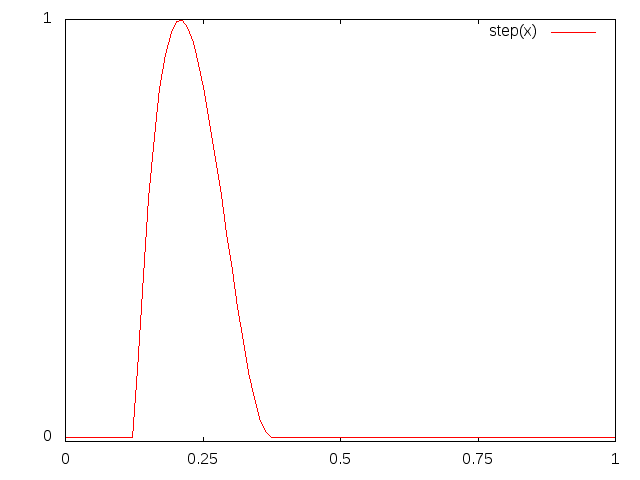
\includegraphics[width=0.5\textwidth]{figures/waveWalkLift}
            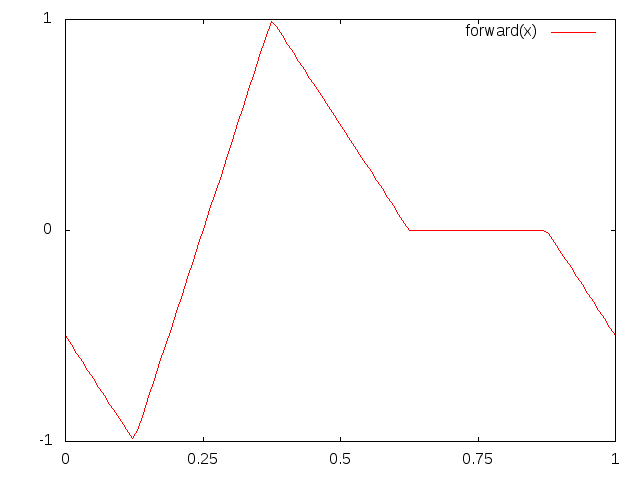
\includegraphics[width=0.5\textwidth]{figures/waveWalkForward}\\
            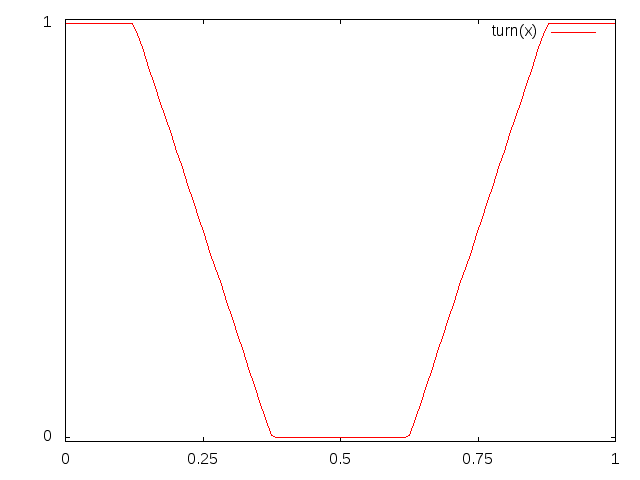
\includegraphics[width=0.5\textwidth]{figures/waveWalkTurn}
            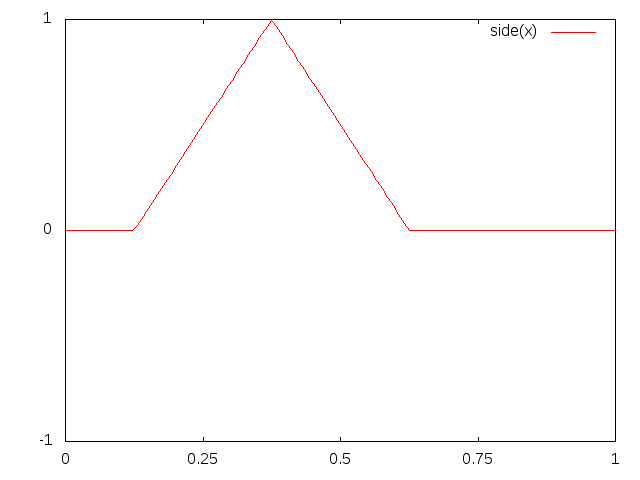
\includegraphics[width=0.5\textwidth]{figures/waveWalkSide}
        \end{tabular}

    \end{center}
    \caption{The functions of WaveWalk. From \emph{top left}, clockwise:
    leg lift; forward step; side step; turn step}
    \label{fig:waveWalkFunctions}
\end{figure}
This is implemented by 5 functions that governs one of these actions, each
only a function of the cycle time. Because they are ssumed to be
independent, they are just superimposed on top of each other as appropriate. They are:
\begin{description}
    \item[Coronal Rock] The WaveWalk rocks the robot in a simple sine wave
        motion. This aims to keep the center of mass within the convex hull
        of the support feet, and allow a reasonable time at each end of the
        rock where the CoM is direcly over one foot. The sine function
        allows maximal speed of transfer and a long dwell time at the
        single support phases.
    \item[Leg Lift] The leg lift function is actually two functions - one
        for the left leg, and one for the right leg that is the same, but
        180\textdegree~out of phase. This is the same for the forward and
        side step functions as well. In both, the leg lift function is zero unless
        the repsective leg is not a support leg. When no weight is on a
        leg, the leg lift function specifies a quick rise and a slower fall
        back to the ground. It is the Langrange polynomial that satifies
        the points $(0, 0)\ (\frac{T}{3}, 1)\ (\frac{2T}{3}, \frac{1}{2})\ (T, 0) $.
        This was used to encourage a softer landing on the ground, thus
        reducing instability. 
    \item[Forward Step] This function specifies the angle of the imaginary
        pendulum extended from the hip to the ankle joint of a leg. Taking
        left foot as an example, it starts with value 0 while it is acting
        as sole support foot. As the robot transitions to double support
        mode, it starts to decrease towards a minimum (parameterised) which
        it reaches when the other foot becomes the support foot. It then
        sharply increases to a maximum by the end of the swing phase,
        moving the leg while it is lifted. The function then decreases back
        to 0 for another support phase.
    \item[Side Step] The side step function is very similar to the forward
        step, except that, as the feet have little space between them, the
        function cannot ever be negative (this would cause the feet to try
        and overlap. The function is simply $\max\left( 0,\
        \textrm{forward}(t) \right)$.
    \item[Turn Step] WaveWalk turns by alternately opening and then closing
        the \emph{LHipYawPitch} joint. To implement this, it uses a
        function that plateaus at $1.0$ during one double support phase, at
        $0.0$ in the other, and linearly transitions between them during
        the single support phases.
\end{description}
\autoref{fig:waveWalkFunctions} shows the leg lift and step functions.


The WaveWalk is also highly parameterised, allowing for the same model to
generate many different style of walk. There are parameters for:
\begin{itemize}
    \item The maximal coronal rock
    \item The spread of the legs when standing
    \item The height of the leg lift
    \item The bend of the legs when standing
    \item The maximal forward, left and turn step sizes
    \item The lift multiplier, which governs how much faster a leg lift
        phase is than the overall cycle
    \item The cycle frequency in Hz
\end{itemize}
These parameters manually tuned, though in future machine learning could be
possible, provided a robust walk testing framework exists.

The WaveWalk was able to attain forward movement of about 8cm/s. This was
better than the old Aldebaran Walk, but with the release of NaoQi 1.6, the
Aldebaran Walk now is capable of 10 cm/s. Additionally, the WaveWalk was
unstable and required a large amount of tuning. This was largely down to
poor design assumptions, like the independence of the five functions, and
also to implementation shortcuts, such as a lack of any proper inverse
kinematics. Hence, the WaveWalk was not used in competition, but was
superseded by FastWalk.

\section{Adaption of Aldebaran Walk}
In NaoQi 1.6, Aldebaran released an omni-directional walk for the Nao. We
decided to use this conjunction with our other walks, switching between
them when necessary. However, this posed a problem, as we could only use
the Aldebaran walk from a NaoQi broker (\textit{i.e.} from libagent), but
walks are meant to be converted to joint angles by a Generator.

This problem is solved by re-purposing some of the fields in JointData to
be interpreted as Aldebaran walk flags. This is safe, because JointData has
fields for position, stiffness and temperature, but temperature is not used
for effecting motions. Thus, libagent can be assured that the field used to
indicate whether to use the Aldebaran walk was not coincidentally set to
the appropriate value.

The Aldebaran walk interface is composed of two parts. Firstly, the
\emph{ALWalkGenerator} translates our omni-directional walk parameters into
the Aldebaran parameters, and stores these in JointValues. Then, this is
eventually passed to libagent. In libagent, if the \emph{AL\_ON} flag is
set, the parameters are read out of the JointValues and passed to ALMotion.

When behaviour requests another action, ALWalkGenerator is sent the stop
signal. It in turn activates the \emph{AL\_stop} flag in JointValues. When
this is read in libagent, it stops processing the walk commands, and
instead transitions back to the standard standing pose, using joint
interpolation. When the interpolation finishes, it sets the
\emph{AL\_isActive} flag in SensorValues to false.

Because we cannot see the internals of the Aldebaran walk, it was
impossible to accurately calculate the odometry data for it on a
step-by-step basis. Instead, we use approximations derived from the
supplied walk parameters. This is usually fairly accurate, but is not
guaranteed to work as ALMotion may not honour the commands.



\section{\emph{SlowWalk} and \emph{FastWalk} Generators}
Two other walks were developed, \emph{Slowwalk} and \emph{Fastwalk}. Slowwalk is an open-loop walk that maintains balance by keeping the center-of-mass over the support polygon  of the stance foot or feet. The speed of joint movement is kept low to avoid undue momentum effects ensuring the center-of-pressure and the center-of-mass projected on the ground do not vary significantly. Fastwalk is a closed-loop walk based on the inverted pendulum model with stabilisation feedback supplied via the foot sensors and accelerometers. Both walks were designed by decomposing the walk phase motion dynamics into their sagittal and coronal planes components and synchronously recombining them. 

Both Slowwalk and Fastwalk are omni-directional walks in that the robot can be directed to simultaneously move forward, sideways and turn. Naturally the combination of these component vectors must be within the physical capabilities of the machine and need to be controlled to keep the robot balanced. Omni-directional foot placement results in a rich variety of movements, for example waltzing backwards. 

Omni-directional locomotion is achieved by moving the swing foot so that
it is replaced on the ground, rotated, and offset in the forward and left
directions relative to the stance leg as shown in \autoref{sectionWalkingParameterisation}. The foot position is specified with three variables, \emph{forward}, \emph{left} and \emph{turn}. Values for these variables are passed as parameters to the walk generator by higher-level skills and behaviours. 

For a given forward and left step-size the walk movement is constrained to move the point on the robot between the hips at a constant velocity over the ground to minimise the acceleration of the body sub-chains above and including the torso. This is thought to reduce forces during the walk cycle, minimise energy usage and oscillatory disturbances. At the same time the legs are moved to achieve the required omni-directional foot placements. To achieve these body, leg and foot movements we calculate new joint-angles each $1/100$ of a second. Determination of appropriate joint angles to position the feet requires inverse kinematic calculations to be performed. We next describe how both close-form and iterative methods were used to calculate joint angles.

\subsection{Inverse Kinematics} \label{sectionIK}
Inverse kinematics determines the robot's joint angles given the desired 3D position of the kinematic chain end-points such as the feet. Both Slowwalk and Fastwalk use two different methods for calculating the joint angles for the walk. A closed-form was used for moving the foot forward, back or sideways. An iterative method for turning was used which involved the more complex hip-yaw joint mounted at 45 degrees to the torso in the coronal plane. We first describe the closed-form followed by the iterative method. 

\textbf{Close-Form Inverse Kinematics}

The stance foot is assumed to be flat on the ground and determines the relative location of all the other joints for a given set of  joint angles. To calculate the joint angles required for walking, we use a coordinate frame centered on the hip joint. The following Slowwalk and Fastwalk \emph{stance} variables are sufficient to describe the state of the walk at any point in time:
\begin{itemize}
\item the position of the center of  each foot in millimetres in the forward direction relative to the hip, i.e. forwardL and forwardR for the left and right foot respectively.
\item the lift of the center of each foot above the ground plan in radians and directly below the hip-joint, i.e. liftL and liftR. Radians may seem an odd way to specify this measure. It represents an additional rotation in the hip-pitch joint, knee-pitch joint and ankle-pitch joint to effect the lifting of the foot in the sagittal plane so that the center of the foot is directly below the hip. 
\item the deviation of the center of each foot in the coronal from vertical in radians. It represents the additional hip-roll required to move the leg sideways. Variables leftL and leftR are used for the left and right leg respectively. 
\end{itemize}

When the \emph{turn} is zero we can use closed-form inverse kinematics to calculate the hip-pitch, hip-roll, knee-pitch, ankle-pitch and ankle-roll of each leg and foot. This is possible because of the unique constraints in Nao's kinematic leg chains. The hip-pitch, knee-pitch and ankle-pitch motors axes of rotation are parallel. Each leg therefore moves in a plane. \autoref{figForwardIK} shows a diagram to visualise the 3D geometry of Nao's legs. We next detail the derivation of all the joint angles. The $*$ symbol in the expressions can be substituted by either $L$ or $R$ for the left or right leg respectively. 
 
\begin{figure} [ht]
\centering
\includegraphics[width=0.8\textwidth]{figures/forwardIK.jpg}
\caption{Geometry of leg position and angles. The * is replaced by either L or R to signify left or right leg variable in the code.} \label{figForwardIK}
\end{figure}

We first calculate the distance between the ankle-joint and the hip-joint when the foot is directly below the hip projected in the sagittal plane. At this point the hip-pitch ($Hp{*}0$) is determined by three terms: the lift of the foot, the crouch (or $legBend$) of the robot which we set at a constant 30 degrees, and a factor for lowering the height of the robot when we take sidesteps. The latter lowers the robot to give it more reach when taking large sidesteps. The hip-pitch for this initial hypothetical position is given by:

\begin{equation}
Hp{*}0    = lift{*} + legBend + (ABS(leftL) + ABS(leftR))/1.5f
\end{equation}

It is now possible to calculate the distance $h*$ between the hip-joint and the ankle-joint from the geometry.

\begin{equation}
h* = (100*cos(Hp{*}0)+ \sqrt{102.74^2 - 100^2*sin^2(Hp{*}0)})/ cos(left{*})
\end{equation}

As the foot is moved parallel to the ground in a forward (or backward) direction by the displacement $forward{*}$ the distance between the hip-joint and ankle-joint increases to $d{*}$:

\begin{equation}
d*  = \sqrt{forward{*}^2 + h{*}^2}
\end{equation}

Given the final distance between the hip-joint and ankle-joint $d{*}$ we can calculate the angles $beta1{*}$ and $beta2{*}$, as shown  in \autoref{figForwardIK}, using the cosine rule to determine the amount the knee-joint needs to bend to achieve $d{*}$.

\begin{eqnarray}
beta1{*}  &=& \cos^{-1}((102.74^2+d{*}^2 - 100^2)/(2*102.74*d{*}))\\
beta2{*}  &=& \cos^{-1}((100^2+d{*}^2 - 102.74^2)/(2*100*d{*}))
\end{eqnarray}

The final hip-pitch is the sum of the angle due to the knee bend plus the angle required to move the leg forward as shown in \autoref{figForwardIK}.  The ankle-pitch is determined similarly to keep the foot parallel to the ground. The knee-pitch is always the sum of the hip and ankle pitch.\footnote{When the foot displacement is significantly behind the hip so that the thigh slopes backwards, the calculations need to be adjusted slightly in sign as reflected in the code.} The joint angles are determined for both legs as follows:

\begin{eqnarray}
HipPitch:Hp{*} &=& beta1{*} + \cos^{-1}(h{*}/d{*})\\
AnklePitch:Ap{*} &=& beta2{*} + \cos^{-1}(h{*}/d{*})\\
KneePitch:Kp{*} &=& {*}HipPitch + {*}AnklePitch\\
HipRoll:Hr{*} &=& left{*}\\
AnkleRoll:Ar{*} &=& -{*}HipRoll
\end{eqnarray}

This completes the closed-form inverse kinematic calculations for forward and sideways movement of the legs. We now address the case when there is also a turn component that is required to change the direction of the robot when walking. 

\textbf{Iterative Inverse Kinematics when Turning}

The hip joints in the Nao are complex in that the hip-pitch, hip-roll and hip-yaw motor axes coincide. The hip-yaw motors in the Nao are required for turning and are inclined at 45 degrees to the torso in the coronal plane. In addition, the left and right motors are constrained to move together by the same amount of rotation --- see \cite{aldebaran10developer}. This increases the complexity of the inverse kinematics for foot placement. 

Our approach is to determine the new hip-pitch and hip-roll angles that leave the position of the ankle-joint unchanged relative to the hip-joint for a rotation of the hip-yaw joint. In this way we can execute a movement of the foot forward and sideways first and subsequently rotate the foot about its center to complete the omni-directional turn. The knee-pitch is left unchanged as the leg is one unit. The ankle pitch and roll is calculated to ensure that the foot is kept parallel to the ground. 

We use a similar iterative inverse kinematic method to that used by Bowdoin College in 2009 based on \cite{Buss04introductionto}. The idea is to iteratively guess the joint angles and perform a forward kinematic calculation until we get close enough to the desired position. The ``guesses" can be improved by considering the local effect on the change in position of the action of each joint movement. This is given by a matrix of partial derivatives called the Jacobian. In this way the guesses can be directed and the number of iterations minimised to achieve the desired final position of the chain. In practice we have found that only three iterations are necessary. 

In particular we use the forward kinematic transform mapping ankle positions into the hip coordinate frame of reference. The derivation of the mDH parameters for the forward kinematic transform is given in \autoref{appendixMDH}, \autoref{appendixNaoKinematicChains} and \autoref{figmDH-leftAnkleToHip}. The Matlab code for the iterative inverse kinematics is provided in \autoref{appendixIKMatlab} and uses \autoref{equationIK} (refer to \cite{Buss04introductionto}) to estimate the change in hip-pitch and hip-roll (vector $\Delta \theta$). 

\begin{equation}
\Delta \theta = J^T(J*J^T+\lambda^2I)^{-1}*\overline e \label{equationIK}
\end{equation} 

where $J$ is the Jacobian providing the change in angle with respect to position, $\lambda $ is a constant (0.4), and $\overline e$ is the displacement between the current position and the desired position. To improve processing speed on the Nao \autoref{equationIK} was expressed symbolically with Matlab and the expressions copied into the C++ code. 

We still need to determine the ankle pitch and roll to keep the foot parallel to the ground. Having determined the location of the ankle joint relative the hip joint, we can use the previous foot-to-hip forward kinematic transform to find the relative position of two points on the foot that are not collinear with the center point  and work out the change in ankle-pitch and ankle-roll to ensure the foot is parallel to the ground. To minimise computations we transform two orthogonal unit vectors from the center of the foot along the foot $x$ and $y$ axes. The ankle angle adjustments are then simply $\sin^{-1} \delta z$, where $\delta z$ is the change in the $z$ coordinate moving along each of the unit vectors.  

This completes the inverse kinematics for one of the legs. The other leg is symmetrical, and we reuse the co-ordinate transform by simply inverting the sign of the hip-roll and ankle-roll. We repeat the above iterative inverse kinematic  procedure for the other leg to complete the full inverse kinematic calculations for all leg and foot joints for the omni-directional walk.  
o

\section{SlowWalk}\label{sectionSlowWalk}

The robot motion \emph{SlowWalk} generator takes the \emph{forward}, \emph{left} and, \emph{turn} and \emph{power}  parameters as input and produces a slow statically balanced open-loop omni-directional bipedal gait for the Nao that shifts the total weight of the robot between the alternate stance feet. Statically balanced means that the robot is balanced at every time-step during the walk even if the speed of gait execution is slowed down to any value. Open-loop means there is not feedback or feed-forward information loop that control the motion. SlowWalk was an early walk development in preparation for the 2010 competition. The walk itself is too slow to be competitive, but it forms the basis of several kicks that require the robot to statically balance on one leg while kicking with the other (see \autoref{sectionSlowWalkKicks}). The power parameter is only used to control kicks. At a value of $0.0$ it invokes the SlowWalk walk.

The SlowWalk gait alternates between a stance phase and swing phase for each leg. It takes 4.2 seconds to complete one complete cycle of the gait, spending 2.4 seconds in two double support phases (in contrast to a FastWalk cycle time  of  0.38 seconds in which almost no time is spent in the double support phase as discussed next in \autoref{sectionFastwalk}).

SlowWalk is described by a task-hierarchy (see \autoref{sectionTaskHierarchy}). The abstract walk phase state transition diagram for the gait is shown in \autoref{figSlowwalkStates}. It should be clear from the diagram how the walk progresses. We start after a reset assuming the robot is in a standing position with its legs together. Motion is generated independently and concurrently in the coronal and sagittal planes. The weight is first transferred to the right foot by moving the torso over the right foot at the same time that the robot rocks to the right. When the weight is over the right foot the robot lifts the left leg (see \autoref{figSlowwakRock} -- right), moves it omni-directionally as shown in \autoref{figOmniStep}  and replaces it. This completes half a cycle. The same procedure is then repeated with the feet reversed. \autoref{figSlowwalkCoP} shows the intended movement of the center-of-pressure (and ZMP) as the walk progresses through the abstract walk phase states. 

\begin{figure}[ht]
\centering
\includegraphics[width=0.8\textwidth]{figures/SlowwalkStates}
\caption{SlowWalk abstract walk phase states.} \label{figSlowwalkStates}
\end{figure}

\begin{figure}[ht]
\centering
\includegraphics[width=0.7\textwidth]{figures/SlowwalkCoP}
\caption{SlowWalk center of pressure trace as the walk progresses.} \label{figSlowwalkCoP}
\end{figure}

Each abstract state is described by a temporally extended action that makes the legs move through several base-level states over a given period of time. The base-level transitions occur at 0.01 second intervals. The temporally extended actions are generated using a sinusoidal function $moveSin(start, finish, period)$ that moves variables from a start position to a finish position in a given period of time as shown in \autoref{figmoveSin}. The intention is to not move abruptly, but to accelerate and decelerate slowly. The moveSin function is written in C++ as follows:

\begin{figure}
\centering
\includegraphics[width=0.5\textwidth]{figures/moveSin}
\caption{Sinusoidal interpolation between start and finish over period used to generate temporally extended actions.} \label{figmoveSin}
\end{figure}

\begin{lstlisting}
float SlowWalkGenerator:: moveSin(float start, float finish,
                                         float period) {
   if ( period <= 0.0f || t < 0 ) return start;
   if ( t > period )              return finish;
   float difference = finish - start;
   float angle = M_PI * t / period;
   return start + difference * (1 - cos(angle))/2.0f;
}
\end{lstlisting}

Transitions between abstract states ensure that the variables values on exit of one state remain unchanged on entering the following state. This is achieved by storing the values between transitions in variables commencing with the string ``last", as in \emph{lastForwardL}, \emph{lastTurnLR}, etc. A typical abstract state implements its temporally extended action by concurrently moving several variables sinusoidally from start to finish in the specified period. At the end of the period it stores the final variable values before resetting the time and flagging the next abstract state for execution. For example the code for rocking the robot from left-to-right and moving forward is:

\begin{lstlisting}
void SlowWalkGenerator::oRockRL(float period, WalkPhase nextPhase) {
   coronalLeanR = moveSin(lastCoronalLeanR, -rock, period);
   coronalLeanL = moveSin(lastCoronalLeanL, -rock, period);
   forwardL     = moveSin(lastForwardL, 0.0f, period);
   forwardR     = moveSin(lastForwardR, -lastForwardL, period);
   leftL        = moveSin(lastLeftL, 0.0f, period);
   leftR        = moveSin(lastLeftR, -lastLeftL, period);
   if (t >= period) {
      lastCoronalLeanR = coronalLeanR;
      lastCoronalLeanL = coronalLeanL;
      lastForwardL     = forwardL;
      lastForwardR     = forwardR;
      lastLeftL        = leftL;
      lastLeftR        = leftR;
      t                = 0.0f;
      walkPhase        = nextPhase;
   }
   return;
}
\end{lstlisting}

The $coronalLean{*}$ moves the hip-roll and ankle-roll joints for both legs
in unison as illustrated in \autoref{figSlowwakRock} (left) shifting the
weight in the coronal plane of the robot onto the left foot. The $forwardL$
variable finishes at value 0 which means that the weight of the robot
should be directly over the left foot after the temporally extended action
operating in the sagittal plane exits. The right foot $forwardR$ will be as
far behind at the finish as the left foot was forward at the start i.e. by value $lastForwardL$. In other words the robot moves forward (or backward) in the process of shifting weight from one foot to the other. If the robot is in the process of moving sideways the extra hip-roll is included in the coronal movements ($left{*}$) preserving any spread of the legs.  Finally, after the period has expired, all the variables involved in this motion are stored at their finish value so that future actions can preserve continuity of the values. Time is reset to zero, ready for the next abstract state (\emph{walkPhase}). The other abstract states have a similar execution method.  A similar interpretation can be made after examining the code.  

\begin{figure}
  \centering
  \begin{minipage}[b]{8 cm}
     \includegraphics[width=0.8\textwidth]{figures/SlowwakRock}  
  \end{minipage}
  \begin{minipage}[b]{8 cm}
    \includegraphics[width=0.8\textwidth]{figures/SlowwalkLeglift}  
  \end{minipage}
  \caption{SlowWalk rock. (left). Leg-lift (right).}
  \label{figSlowwakRock}
\end{figure}

At $1/100$ second intervals the base level state variables values specifying the stance of the robot are passed to the inverse kinematic functions described in \autoref{sectionIK} to determine all the joint angles. 

The SlowWalk generator executes the following steps 100 times per second:
\begin{enumerate}
\item Scale back any ambitious \emph{forward}, \emph{left} and \emph{turn} parameters to manageable values. We need to protect the integrity of the walk in case higher level components in the task-hierarchy make unreasonable requests that cannot be physically realised.
\item Reduce the leg-lift-height proportional to the amount of \emph{left} and \emph{turn} requested. Walking sideways and turning motions are improved by lowering the stance of the robot to allow a further stretch and hence reach of the legs and reducing the lift respectively. 
\item Update odometry. This output from the generator is used by the Bayesian filter process model for localisation (see \autoref{figrunswift2010architecture}).
\item Update the robot stance variables depending on the current abstract action (walkPhase) as described above.
\item Determine the joint angles from the stance variables using inverse kinematics as described in \autoref{sectionIK}.
\item Return the joint angles for writing actuation requests via the DCM.
\end{enumerate}

\section{FastWalk} \label{sectionFastwalk}

FastWalk generates omni-directional dynamically stabilised closed-loop bipedal robot motion. As the name suggests this walk is faster than SlowWalk --- by about an order of magnitude.  After summarising the overall process steps of the generator and the task-hierarchy that generates the walk, we will describe the walk dynamics by appealing to a simple inverted pendulum model and discuss the feedback control mechanisms.

\subsection{Process Steps of the FastWalk Generator}
We enumerate the steps in the overall FastWalk process. They follow the structure of the source-code:
\begin{enumerate}
\item Assign new \emph{forward}, \emph{left}, \emph{turn}, and \emph{power} parameter values. These parameter values are passed to the FastWalk generator from skill and behaviour components higher in the task-hierarchy.
\item If FastWalk has been asked to $stop$ and is therefore in the process of \emph{stopping} we set the \emph{forward}, \emph{left}, and \emph{turn} parameters to zero, just in case the parent tasks are still sending non-zero values. 
\item \emph{Power} is used to set the limit on the absolute value that the \emph{forward} parameter can take. The purpose is to allow parent skills and behaviour tasks to set the maximum speed of the walk, but accepting a higher risk of falling over. 
\item When the parent tasks requests FastWalk to simultaneously walk \emph{forward} and \emph{turn} at a rate that is not achievable or that runs a high risk of falling, FastWalk gives precedence to the $turn$ request. If the \emph{turn} is requested when in full stride, the $forward$ speed is first reduced before the $turn$ is increased.
\item The $targetWalkPatter(forward, left, turn)$ function moves the current state of the walk in terms of $forward$, $left$ and $turn$ incrementally closer to target values as determined above. A key feature of FastWalk is that the walk parameters are adjusted slowly over the whole walk cycle rather than being set at specific time-points. 
\item The center-of-pressure is calculated separately in the coronal and sagittal directions for each foot using the equation in \autoref{figZMP}. As there are four distinct foot-sensors on each Nao foot that we treat as point pressure detectors, the integral is replaced by a sum.
\item The coronal and sagittal center-of-pressure, together with the inertial measurement unit x-accelerometer readings are filtered at several frequencies for later stabilisation of the gait (see Feedback Control --- \autoref{sectionFastWalkFeedbackControl}).
\item The cycle timer is updated by $1/100$ of a second.
\item If the combination of the requested weighted magnitude for $forward$, $left$ and $turn$ is greater that the scaled limit of any one of these variables, they are scaled back in proportion to their weighting in an attempt to avoid high-risk motions.
\item We adjust the forward parameter of the left and right foot so that when the robot is simultaneously moving forward and turning, the inner foot to the turn circle moves forward at a slower rate than the outer foot. 
\item The robot is stabilised coronally based on the zero-crossing point of the center-of-pressure estimate (see Feedback Control below)
\item Update odometry. Output from the generator is used by the Bayesian filter process model for localisation (see \autoref{figrunswift2010architecture}). We have found there is generally a 0.9 slip for each of \emph{forward}, \emph{left} and \emph{turn}. We have not calibrated odometry for various combinations of parameters.
\item The walk is stopped and reinitialised if in the process of stopping and the current state of \emph{forward}, \emph{left} and \emph{turn} are all zero.
\item The current state of \emph{forward}, \emph{left} and \emph{turn} is reset at each half-cycle to insure it is in step with the walk. As this is a closed-loop walk the cycle length may change. Accelerating and decelerating in any of \emph{forward}, \emph{left} and \emph{turn} during the cycle can also cause the gait to become asymmetric. This function is crucial to keep the walk gait in the sagittal plane synchronised.
\item Update the robot stance variables depending on the current abstract action (walkPhase) in the task-hierarchy --- see \autoref{sectionFastwalkTaskHierarchy}.
\item Determine the joint angles from the stance variables using inverse kinematics as described in \autoref{sectionIK}.  
\item If there is minimal pressure on the feet, assume the robot has fallen over or has been picked up. Reset the joint angles to the standing position at low stiffness. 
\item Return the joint angles for writing actuation requests via the DCM.
\end{enumerate}

\subsection{FastWalk Task-Hierarchy}\label{sectionFastwalkTaskHierarchy}
FastWalk is represented as a two level task-hierarchy in \autoref{figFastwalkTaskgraph}. The top level invokes foot-lift and omni-directional foot-placement motions for the left and right legs triggered at set times during the walk cycle as shown in \autoref{figFastwalkGaitCycle}.
\begin{figure}[ht]
\centering
\includegraphics[width=0.6\textwidth]{figures/FastwalkTaskgraph}
\caption{FastWalk task hierarchy.} \label{figFastwalkTaskgraph}
\end{figure} 

\begin{figure}[ht]
\centering
\includegraphics[width=0.6\textwidth]{figures/FastwalkGaitCycle}
\caption{FastWalk gait cycle.} \label{figFastwalkGaitCycle}
\end{figure} 

At time $t=0$ the robot initiates the left leg phase of the gait and at time $t=T/2$ the right leg. The foot-lift and foot-placement timing in the left and right cycles of the gait is determined by the $liftFrac$ and $movFrac$ parameters that give the fraction of the total time devoted to lifting the foot and placing it omni-directionally. The lifting and moving sub-tasks are initiated so that they are centered time-wise in each half-cycle. The start of the foot-lift action, for example, is calculated as  $startT = ((1-2*liftFrac)/4)*T$. A similar calculation initiates the foot placement action.  FastWalk uses $liftFraction = 0.5$ and $movFrac = 0.4$. This means that 100\% of the time the left and right phase executes the lifting motion, but only 80\% of the time is allowed for placing the feet. The effect is that the foot is lifted first before it is moved in an attempt to provide some margin to avoid moving a foot that is still on the ground. 

We tried various sinusoidal and quadratic loci for lifting and moving the feet. We settled on a sinusoidal lifting action (as for SlowWalk --- see \autoref{figmoveSin}) attempting to replace the foot gently on the ground. For the omni-directional foot placement we used two parabolas back to back. The rational for the parabolic functions is that it optimises the displacement given an assumed maximum acceleration/deceleration allowed by the friction of the feet on the carpet. In this case, it is optimum to accelerate at the maximum rate to the half-way point and then decelerate to a full-stop during the second half. The velocity increases and then decreases linearly, with the displacement increasing/decreasing quadratically. Each component, $forward$, $left$, and $turn$ uses the this function scaled appropriately. 

\subsection{Inverted Pendulum Dynamics}
The walk is designed by first dividing the dynamics into its orthogonal (coronal and sagittal plane) components and recombining the two motions synchronously to generate bipedal motion. The walk dynamics can be understood by appealing to an inverted pendulum model of the Nao. 

\begin{figure}[ht]
\centering
\includegraphics[width=0.5\textwidth]{figures/FastwalkCoronalRock.jpg}
\caption{FastWalk oscillation in the coronal plane showing the dynamics modelled by inverted pendulums with their pivot points located on the edges of the feet.} \label{figFastwalkCoronalRock}
\end{figure}

\textbf{Coronal (or Lateral) Dynamics}. \autoref{figFastwalkCoronalRock} shows a coronal view of a stylised Nao with the whole mass concentrated at the center-of-gravity (CoG), shown as the red dot in the torso. Each of the flat feet is lifted vertically during the walk, the lift being parameterised by the two variables $liftL$ and $liftR$ introduced in \autoref{sectionIK}. The idealised robot will only make contact with one of four points projected in the coronal plane when rocking from side to side. The four points correspond to the outside and inside edges of the feet. We therefore model the robot as an inverted pendulum with its bob at the CoG and the pivot point at one of the feet edges. As the robot rocks from side to side the pivot point of the pendulum switches depending on which edge touches the ground. In the figure, the depiction on the right shows the robot making contact with the inside left-foot. 

\begin{figure}[ht]
\centering
\includegraphics[width=0.5\textwidth]{figures/InvPen.jpg}
\caption{The gravitational force on the bob of an inverted pendulum has a component in the perpendicular direction to the rod proportional to the $\sin$ of the angle the rod subtends to the vertical.} \label{figInvPen}
\end{figure}

The force acting on the bob of an inverted pendulum in its direction of motion is $mg\sin(\theta)$ as shown in \autoref{figInvPen}. We start with an idealised system where total momentum, and hence the magnitude of velocity, is conserved. Each time the pendulum changes pivot we assume the impact results in a loss of energy which we have simply modelled by reducing the velocity of the bob by a small fraction. Energy is added to the system implicitly when the feet push down and lift the robot. We model external disturbances by changing the velocity on impact by a small random quantity with zero-mean. An example time-series plot for the center-of-pressure (the blue squarish wave) and a regular sinusoidal foot lifting action (red wave) for the simple inverted pendulum model of the Nao is shown in \autoref{figSimpleInvPenNaoOpenLoop}. The foot-lift plot shown in red is positive when the left foot is lifted and negative when the right foot is lifted.  The CoG acceleration alternates from left to right by the alternating foot lift action as the pivot of the pendulum changes from foot to foot.   

\begin{figure}[ht]
\centering
\includegraphics[width=0.9\textwidth]{figures/SimpleInvPenNaoOpenLoop}
\caption{The simple inverted pendulum model of the Nao showing an example CoP (blue) and foot-lift (red) time-series for an open loop walk.} \label{figSimpleInvPenNaoOpenLoop}
\end{figure}

In the open-loop setting, the timing of the leg lifting action is independent of the state of the rock. External disturbances without feedback or feedforward can cause the robot to loose balance and fall over as shown in \autoref{figSimpleInvPenNaoOpenLoop}. Here, towards the end, the sinusoidal action of  the feet continues despite the robot being poised on one leg. Our aim is to control the leg-lift motion to stabilise the rock. We describe this in the \autoref{sectionFastWalkFeedbackControl}, but first discuss the dynamics in the sagittal plane. 

\begin{figure}[ht]
\centering
\includegraphics[width=0.5\textwidth]{figures/FastwalkSagittalMotion.jpg}
\caption{The simple inverted pendulum model of the Nao for the sagittal plane.} \label{figFastwalkSagittalMotion}
\end{figure}

\textbf{Sagittal Dynamics}. The inverted pendulum model for the sagittal plane is shown in \autoref{figFastwalkSagittalMotion}. The pivot of the inverted pendulum is again at one of the edges of the feet, this time either at the front or the back. The forces on the robot are determined by the pivot edge and the angle of the rod from the pivot to the CoM ($\theta$ in the figure). The stance and swing feet angles to the torso are kept to the same magnitude ($\beta$ in the figure), and controlled by the left and right foot $forward$ parameters. The feet are inclined so as to keep them parallel to the ground plane. For a walk at constant velocity the CoP should stay between the rear and front edges of the stance foot with the torso in a vertical position. If the robot sways forward or backward, ($\alpha$ in the figure), we detect this with either the foot-senors or the $x$-accelerometer in the chest, and use these observations to help control the balance of the robot.  


\subsection{Feedback Control}\label{sectionFastWalkFeedbackControl}
Both the coronal and sagittal dynamics of Fastwalk have been stabilised to reduce the incidence of Fastwalk falling over. We next describe both the method and results for the stabilisation of Fastwalk in both coronal and sagittal planes with the simulator and for the real Nao robot.

\textbf{Coronal Rock Stabilisation}
The coronal rock is stabilised by synchronising the onset of the leg-lift motion with the switch in stance and support foot. We switch the stance and support feet by observing the zero-crossing of the measured CoP. The CoP is calculated in the coronal plane with the origin in the middle of the robot between the feet. It is negative when the robot stands on the right foot and positive when it switches to the left foot. The period that the robot spends on the stance foot cannot be determined precisely when there are disturbances such as uneven surfaces, play in motor gears, dirt on the ground, and bumping by other robots. The zero-crossing point of the CoP indicates that the robot is just shifting it weight to the other leg. We use it to reset the starting time for both the left and right swing phases of the walk cycle. The FastWalk code to achieve is listed below, where $lastZMPL$ is the filtered coronal CoP at the previous time-step, $filZMPL$ is the filtered coronal CoP this time-step, $t$ is the current time-step, $leftPhase$ is true if the left leg is the swing leg and false if the right leg is the swing leg, and $T$ is the set period of time for one complete walk cycle. $T$ is set at 0.38 seconds, but the actual period of each walk cycle may vary from cycle to cycle depending on the control algorithm.  

\begin{lstlisting}  
   // Controller to stabilise/synchronise walk coronally
   if (lastZMPL > 0.0f && filZMPL < 0.0f) {
      t = 0;
      leftPhase = true;
   }
   if (leftPhase && t > T) t = 0.0f;
   if (lastZMPL < 0.0f && filZMPL > 0.0f) {
      t = T/2.0f;
      leftPhase = false;
   }
   }
   if (!leftPhase &&  t > 1.5f*T) t = T/2.0f;
   }
\end{lstlisting}  

\begin{figure}[ht]
\centering
\includegraphics[width=0.6\textwidth]{figures/FastwalkCoronalRockCosedLoop}
\caption{Simulated closed-loop coronal rock using the CoP zero-crossing point. The time series show the CoP and the leg-lift actions over time.} \label{figFastwalkCoronalRockCosedLoop}
\end{figure}

\begin{figure}[ht]
\centering
\includegraphics[width=0.5\textwidth]{figures/FastwalkRealCoPLift}
\caption{Real Nao closed-loop coronal rock using the CoP zero-crossing point.} \label{figFastwalkRealCoPLift}
\end{figure} 

The controlled inverted pendulum model stays balanced for a significantly longer period of time. The CoP and leg-lift time series for the closed-loop coronal rock is show in \autoref{figFastwalkCoronalRockCosedLoop}. In comparison with \autoref{figSimpleInvPenNaoOpenLoop} it can be seen that the motion has a more consistent period with the onset of the leg-lift action either delayed or brought forward. 

The same controller running on the real Nao produces the time-series for the CoP and leg-lift as shown in \autoref{figFastwalkRealCoPLift}. It is easy to see the similarity between the results from the simulation and from real robot, even though the inverted pendulum model is very basic. The real Nao was tested on a felt carpet which may explain the ragged edges on the CoP measurement over 8 foot sensors. 

\textbf{Sagittal Stabilisation}
The real Nao robot is stabilised in the sagittal plane by leaning the torso (including the head and arm kinematic chains) forward or backward in response to feedback measurements of sagittal CoP and acceleration and feedforward head-pitch settings. The lean was controlled by changing the both the left and right hip-pitch angles. As the head has a significant mass (476.71 grams), the change in the CoG when tilting the head forward is compensated by leaning the robot backward ($headPitchAdj$).  

The three feedback components are:
\begin{itemize}
\item Low frequency response to the CoP
$$\textrm{filLowZMPF} = 0.99*\textrm{filLowZMPF} +
0.01*DEG2RAD(\textrm{ZMPF}*0.01)$$
The motivation for this component is to compensate for any time invariant bias
each robot might have to lean forward or back.
\item High frequency response to the CoP
$$\textrm{filHighZMPF} = 0.8*\textrm{filHighZMPF} +
0.2*DEG2RAD(\textrm{ZMPF}*0.03)$$
This signal was used to counteract any unwanted rocking motion.
\item Filtered acceleration in the x-direction
$$\textrm{filAcc} = 0.5*\textrm{filAcc} + 0.5*(DEG2RAD(\textrm{acc}*0.2))$$
This signal was also used to counteract any unwanted rocking motion. 
\end{itemize}

The filter magnitudes and gains adjusted empirically in order to bring the lean of the robot ($\alpha$ in \autoref{figFastwalkSagittalMotion}) to zero in the smallest number of time steps --- otherwise known as \emph{dead beat control}.   The feedback for these three components was applied to the hip-pitch as follows:
\begin{lstlisting}  
j.angles[Joints::LHipPitch]    = -HpL-filHighZMPF+headPitchAdj
                                    +filLowZMPF-filAcc;
j.angles[Joints::RHipPitch]    = -HpR-filHighZMPF+headPitchAdj
                                    +filLowZMPF-filAcc;
\end{lstlisting}    


\subsection{FastWalk Development}
During development FastWalk time-series were plotted to examine the state of  the walk. We tuned the parameters of the walk manually by observing the plots and the behaviour of the actual robot. Several issues were addressed in this way. A bug was discovered by observing the plots where the forward step-size of one leg increased irrespective of whether the robot was turning left or right. This was not notice by observing the behaviour of the robot and may have been camouflaged by the stabilisation. \autoref{figFastwalkBugFix}  shows the before and after effect for the bug was fix. 

\begin{figure}[ht]
\centering
\includegraphics[width=0.6\textwidth]{figures/FastwalkBugFix}
\caption{Step-size Bug. The top diagram shows that one leg (green graph) would increase in stride-length whether the robot was turning left or right (purple graph). The bottom diagram shows the effect of fixing the bug. A left turn would now reduced the stride-length (green graph) of the left foot and increase it for a right turn. (Note, some variables are scaled differently for each diagram).} \label{figFastwalkBugFix}
\end{figure} 

\begin{figure}[ht]
\centering
\includegraphics[width=0.8\textwidth]{figures/FastwalkTurnAtHighSpeedBefore}
\caption{Turning at high speed causes instability --- note CoP (red) and Acceleration (black) plots.} \label{figFastwalkTurnAtHighSpeedBefore}
\end{figure} 

\begin{figure}[ht]
\centering
\includegraphics[width=0.8\textwidth]{figures/FastwalkTurnAtHighSpeedAfter}
\caption{Turing at high speed after modifying the program as described in the text.} \label{figFastwalkTurnAtHighSpeedAfter}
\end{figure} 

Another example was the analysis on instability when attempting a turn at high speed. By adjusting the onset of the turn and decreasing the rate of deceleration were able increase the stability of the walk. \autoref{figFastwalkTurnAtHighSpeedBefore} and \autoref{figFastwalkTurnAtHighSpeedAfter} show several time-series from a real Nao under feedback control walking at high speed in a forward direction ($left$ and $right$ plots) and then given a command to turn sharply to the left. To stabilise this action, the speed is reduced before executing the turn. The red and black graphs show the response of the CoP and accelerometers respectively. The increase in the CoP is caused by the decelerating robot as it tips forward putting more pressure on the front edges of the feet. As the robot leans forward on deceleration the x-accelerometer also shows an increase. The sway is corrected and both quantities dip before stabilising again.

\section{Omni-directional Kick}
In 2009, rUNSWift used a static, forward-only kick in the competition.
While this worked well, in 2010 we aimed to expand the kick to be able to
kick in other directions. One attempt at this was to build an
omni-directional kick that would be able to kick in any direction within a
specified range, and would also be able to kick balls that weren't just
directly in front of it, but also slightly to the side. This would make the
robot's kicks more like a human player.

The \emph{KickGenerator} is responsible for performing omni-directional
kicks. It uses a state-based model with several states, some of which are
static and some of which are dynamic. The model uses 6:
\begin{description}
    \item[Lean (static)] This is when the robot shifts its centre of mass
        onto its non-kicking leg.
    \item[Lift (static)] The leg is lifted into the air.
    \item[Line-up (dynamic)] The leg is lined up to the position of the
        ball (along the robot's coronal axis), and rotates if kicking at an
        angle.
    \item[Kick (dynamic)] The swing of the kick is executed.
    \item[Un-line-up (static)] The robot returns the leg to a neutral position,
        still off the ground.
    \item[Un-lean (static)] The robot transfers its CoM to both feet and
        lowers its kicking foot.
\end{description}

KickGenerator is capable of kicking balls forward if the balls are between
50mm (in front of a foot) and 120mm to either side of the centre of the
robot (as defined by the omni-directional kick parameters in
\autoref{sectionOminDirectionalKickingParameterisation}. It can kick at
angles, but does not corectly calculate the offset in foot position
required. For instance, kicking at 45\textdegree~with foot at 50mm will
actually kick a ball at about 20mm or 80mm (depending on whether kicking
left or right). It can also only kick with the tip of its foot; future work
might include extending this to use the side of the foot to kick at large
angles (beyond the limits of the LHipYawPitch joint).

KickGenerator was not used in competition, as its omni-directionality was
incomplete, and as a forward kick, it was superseded by the SlowWalk
forward kick. Its main disadvantages are that it does not kick particularly
hard (maximum of 4 metres), and that it takes a long time to execute,
risking the ball being stolen by opponenents.
\section{SlowWalk Kicks} \label{sectionSlowWalkKicks}

SlowWalk (\autoref{sectionSlowWalk}) is able to make the robot balance indefinitely on one leg, motivating its deployment for kicking, as it left the other  foot free to swing at the ball. Each of the kick types invokes SlowWalk to rock onto either the left or right foot, stop, and then execute a series of motions with the swing foot designed to kick the ball in different directions. The kicks can be represented by a four-level task-hierarchy --- 
\begin{description}
\item[Level 1] initiates each kick choosing the power of the kick base on the power parameter passed to the SlowWalk generator by higher level skill and behaviour tasks.
\item [Level 2] executes the SlowWalk abstract walk phases (see \autoref{figSlowwalkStates}) invoked by Level 1. The omni-directional foot-placement subtasks, \emph{move-left-foot-forward} and \emph{move-right-foot-forward} in SlowWalk, are replaced by multi-phase movement routines designed to kick the ball. 
\item [Level 3] represents the sequence of phases that move the foot, etc., to line up the ball, kick the ball, and return the foot to its starting position.
\item [Level 4]  generates arm, leg and foot position states at 100Hz, implementing each phase at level 3. We use sinusoidal (see \autoref{figmoveSin}) trajectories for smooth acceleration and deceleration of the joints.   
\end{description}

\begin{figure}[ht]
\centering
\includegraphics[width=0.8\textwidth]{figures/SlowWalkKickTaskHierarchy}
\caption{Part of the SlowWalk kick task-hierarchy showing a forward kick with the right leg.} \label{figSlowWalkKickTaskHierarchy}
\end{figure} 

\subsection{The Forward Kick --- An Example}
Part of the task-hierarchy (for a \emph{Forward-Kick} with the right leg) is shown in \autoref{figSlowWalkKickTaskHierarchy}. Task-hierarchies are described in \autoref{sectionTaskHierarchy}. We will follow the execution, of an example forward kick with the right leg, through the task-hierarchy in detail. The other kicks follow a similar pattern and can be interpreted from the detail in the code. 

At level 1, kicks are initiated with the $forward$, $left$, $turn$ and
$power$ variables passed to SlowWalk from higher level skill and behaviour
subtasks. Their interpretation is overloaded and follows the
omni-directional kicking parameterisation in \autoref{sectionOminDirectionalKickingParameterisation}. For kicking, the usual
SlowWalk $forward$, $left$, $turn$ values used for walking are set to zero.
A $power$ setting greater than 0.01 invokes a kick. To kick a ball in the
forward direction with the right leg requires the ball to be in front of
the right foot (i.e. at $forward=135mm$, $left=-60mm$). It is up to higher level sub-tasks to insure that this is the case. $Power$ sets the strength of the kick. The strength of a kick is set by a parameter ($kickPeriod$) specifying the duration of the \emph{Kick Action} subtask at level 3. The acceptable range of kick strengths are determined empirically to provide soft kicks and hard kicks near the limit of stability of the kick mechanism. For the forward kicks, $kickPeriod = 0.9 - power * 0.5$, where $power \in (0.01,1.0]$.

Level 1 kick initiation selects the kick type ($kickPhase$) and the $walkPhase$ entry point in the level 2 subtask. In our example $walkPhase = RockRL$, causing the robot at Level 2 to put all its weight on the left foot and then lift the right foot in the usual SlowWalk fashion before invoking the kick at Level 3.

Level 3 has three subtasks: draw the foot back, kick and replace the foot. The period of execution for the first and third subtask is 0.14 seconds, the second kick-action subtask's period is determined by the $kickPeriod$ (see above).
In each subtask, the arms are moved to provide some counter-balance to the rapid leg movements as the foot is lifted and moved forward and backwards. Each movement trajectory is generated by following a cosine function resulting in Level 4 states that represent final joint angles. For example, the action to move the foot from 60mm behind to 140mm forward to kick the ball is 

\begin{equation}
forwardR = -60.0 + 140.0 * (1 - cos(angle))/2.0
\end{equation}

where the angle sweeps from 0 to $\pi$ radians in the time period specified for this kick action. Other movements and actions follow similar lines and we advise the reader to consult the code for details.  

\subsection{Other Kicks}
Left, right, passing and backward kicks are implemented in a similar fashion. $Backward$ kicks and $passing$ kicks require one foot to move next to the ball to allow the other foot to perform its function. In the backward kick the kicking foot needs to step over the ball. 

The passing kick is designed to allow the foot to have a longer period of contact with the ball (rather than an impulse), to reduce the variance of the distance the ball travels. The power setting for the passing kick is different to other kicks with an attempt made to make the power setting proportional to the kick distance. The rational  is that if kinetic energy of the ball is dissipated at a constant rate by carpet friction and initial velocity of the ball is determined by the period of the kick set using power, then a period inversely proportional to the square root of power would theoretically determine the length of the kick.     

\subsection{Results}
Kick variability was tested on the real robot by running a kicking behaviour that would approach and line up the ball and then kick the ball at a certain power setting. A sample of about 10 to 13 balls were used at several power settings. The final position of all the balls gave a particle pictorial representation of the probability distribution of the kick's potential.

\begin{figure}[ht]
\centering
\includegraphics[width=1.0\textwidth]{figures/SlowWalkSideKickDistributions}
\caption{Distribution of balls for thirteen SlowWalk sideway kicks for several \emph{power} settings.} \label{figSlowWalkSideKickDistributions}
\end{figure} 

\autoref{figSlowWalkSideKickDistributions} shows example distributions for 13 right-sideways kicks executed with the Nao standing on the outside goal-box line and kicking towards the center of the filed. The closer distributions have been biased by balls rolling into each other and understate the result.  


\section{Other Motions} \label{posFiles}
There are several other actions that a robot might need to make during play
or debugging. For most of these, a scripted movement is specified using
\texttt{.pos} files, which is then executed by the \emph{ActionGenerator}.
For a few actions, a dedicated generator is required, usually due to the
inadequacies of the \texttt{.pos} file syntax.

A \texttt{.pos} file is composed of at least one line, each with joint
angles (in degrees) for each joint in the robot, separated with spaces. At
the end of each line, there is a duration field that specifies how long the
transition into that state takes in milliseconds. Lines can be comments if
their first character is a hash (\texttt{\#}).

\begin{figure}[ht]
    \begin{center}
        \small
        \begin{verbatim}
# HY HP LSP LSR LEY LER LHYP LHR LHP LKP LAP LAR RHR RHP RKP RAP RAR RSP RSR REY RER DUR
  0  0  90  0   0   0   0    0   -30 60  -30 0   0   -30 60  -30 0   90  0   0   0   1000
        \end{verbatim}
    \end{center}
    \vspace{-25pt}
    \caption{An example \texttt{.pos} file.}
    \vspace{-15pt}
    \label{fig:pos_syntax}
\end{figure}

\subsection{Get-ups}
The robots perform the standard get-up actions, but with the step times
used by B-Human in 2009\cite{thomas09code}. This is much faster than the
original versions, while still being mostly reliable.

\subsection{Initial Stand}
When the robot is first stiffened, a special initial action is performed.
It slowly transitions the robot from the position it was in when it was
stiffened to the standard stance. This prevents robot damage, as otherwise
a joint might otherwise move at maximum motor speed into position.

\subsection{Goalie Sit}
There is a special action so a player can crouch down when they are not
moving. This was intended to prevent excessive overheating, especially of
the goalie. When executed, it slowly crouches the robot down. When another
action is requested, it first slowly stands the robot up again to avoid a
jolt to the robot.
\section{Joint Sensors}
Of the joint sensors provided, both the position and temperature are read
from ALMemory. The current and acknowledgement sensors are however ignored.
These sensors are read at 100 Hz and reported directly to the rest of the
system without any filtering, as we found the sensors to be quite accurate
and reliable.

\section{Chest and Foot Buttons}
The chest and foot button sensors are used for debugging inputs, and to
implement the ``button-press'' interface to the Game Controller. Foot
buttons are handled as simple sensors, being read at 100Hz and reported
straight to the rest of the system without any processing. For these, a
value of 1.0 indicates that the button is depressed; 0.0 indicates it is
released. Each foot button actually consists of two sensors -- no effort is
made to hide this and the user of the values should combine them if this is
desired. They are used mainly as modifiers to chest button clicks, similar
to the Shift key on a keyboard.

The chest button is dealt with slightly differently. It is assumed that the
input for the chest button is a number of quick consecutive taps (similar
to a double-click on a mouse). The libagent module keeps track of these
presses, and when one is detected, it starts a counter. Every press then
increments this counter, until the period of release of the button exceeds
180 ms. Then the \emph{click} is considered by libagent, and if it is one of
the types of click accepted by libagent for debugging, is processed.
Otherwise it is passed to runswift. It is impossible for both libagent and
runswift to receive the same length of click.

\section{Inertial and Weight Sensors}
The Nao robot provides several sensors for detecting the balance of the
robot's mass. There is a three-axis accelerometer (accuracy $\pm 1 \%$), a two-axis gyroscope (accuracy
$\pm 5 \%$), and four force sensitive resistors on each foot, that report
the weight applied to them (accuracy $\pm20\%$).

All of these values are read at 100 Hz and directly passed on to the rest
of the system. It would have been beneficial to do some filtering of these
in Motion, but this is currently delegated to the users of the data.

\section{Sonar}
The ultrasound system on the Nao has changed with this year's version of
the robots. The new system allows both sensors to run continuously every
100 ms, recording up to 10 echoes for each sensor. The minimum range of the
sensors is 0.3 m, \emph{i.e.} if an object is closer than 0.3 m, its
distance will be reported at 0.3 m regardless. The maximum theoretical
distance the sonar can detect is 2.54 m; however, we found the values to be
highly unreliable at distances over 1 m.

Occasionally, we found that the ultrasound sensors would stop working and
return a distance of 0.02 m constantly. This was especially frequent after
flashing one of the robot's control board. The solution to this was usually
just to restart the robot. Since the problem sometimes occurred mid-match,
there is a routine to detect if this occurs and vocally warn the user
(using \texttt{flite}).
\section{Sonar Filter \label{sectionSonarFilter}}
At the behaviour level we need to use data obtained via the Sonars to determine if we are about to collide with an object in front of us.

In its first iteration the Sonar filter used a simple low gain filter in an attempt to smooth out the raw Sonar data. This filter worked well for objects that were close but had trouble detecting objects that were further than 50cm away. This was due to Sonar spikes in which the object was not detected in some frames causing the filter to overestimate the objects distance. Due to time constraints we never optimised this filter and its limitations were noticed in our first three games at competition.

In these games we appeared to detect enemy robots too late and occasionally walk into them. Other times we would detect them too early and start avoiding the robot prematurely.

Half way through competition it was decided to implement a new filter to correct this. We settled on a filter that kept a history of the last 10 sonar values. At each iteration it then looped over these 10 values and if 8 of these were less than 60cm we then decided that an object had been detected. The two values of 60cm and 8 readings were hand tuned at competition and since then no work has been done to determine if this was in fact any better than our low gain filter. Perhaps adjusting the gains of our old filter will fix them.

Implementing an effective sonar filter should be a priority for next years team.

\section{Discussion}
One of the main principles behind the motion architecture is that all
motions are generated by separate generators, and that to transition
between them, they must go through the standing pose. This is clearly
inefficient, but was imposed for ease of development. A better system would
either allow multiple transition poses, or leave responsibility to
transition up to the incoming generator, or even dispense with separate
generators and have one generator that does everything.

Another design decision was to use multiple walks---a FastWalk for long
distance, straight-line walking and the Aldebaran Walk for short-distance,
omni-directional walking. This was partially successful, but much of the
code was not written this way, with the FastWalk being used even if it was
sub-optimal (especially when sidestepping). The solution going forward is
to abandon the Aldebaran Walk and devise a fully omni-directional walk that
has the forward speed of the FastWalk.

While we had planned to develop an omni-directional kick, this was never
fully completed, and instead we used a set of scripted kicks for various
angles. This was satisfactory for the competition, but omni-directional
kicks would save the robots from having to rotate about the ball before
kicking it.

There is also a lot of duplication in the Motion system, with three walks
and two kicks. This is in part due to our development approach of ``fail
fast, fail cheap'', which stresses rapid development, even if this leads to
abandonment of one approach in favour of another later.

\section{Future Work}
There are several improvements that can be made to the Motion framework to
improve it in 2011:
\begin{description}
    \item[Smooth switching between motions] Actions should be able to be
        switched between without always having to transition via the
        standing pose. This may be achieved by integrating the kick, walk
        and dribble actions into one cohesive generator.
    \item[Machine-learned motion parameters] In 2010, all walks were
        manually tuned, though they were parameterised to some extent. This
        can be leveraged in 2011 to perform gradient-descent optimisation
        on the walk, especially if it can be opened up with more parameters
        than currently specified.
    \item[True omni-directional kick] In 2010, some progress towards an
        omni-directional kick was made, but was never completed or used.
        This work should be continued in the future, as an omni-directional
        kick would be both good for behaviour and good for the goal of the
        league, as omni-directional kicking is one human aspect that is yet
        to translate to the robotic game.
    \item[Stabilisation of actions using inertial sensors] In 2010, the
        inertial sensors were largely ignored, except to determine if the
        robot was lying on the ground or not. In future, they should be
        studied and used to implement damping for all motions. This will
        make them more stable if we are pushed, which is a benefit as it
        saves the time required to execute a get-up motion.
\end{description}

\section{Conclusion}
The Motion system was a large contributor to rUNSWift's overall success in
the competition. The high speed of our main walk, FastWalk, at 22 cm/s,
allowed our robots to outpace most other teams and nearly match the fastest
teams. The adaption of the Aldebaran walk meant that we were always no
worse off than the baseline and provided an important safety-net. The kicks
were highly tuned and delivered with accurate and fast shots. The sensor
values were under-utilised, but the ultrasound was highly effective in
avoiding other robots (and hence pushing penalties), especially when
filtered. Our work this year sets a solid base for future teams to build
upon, with a reliable but flexible architecture.

% **********************************************************************************************************
\newpage
\chapter{Behaviour}\label{sectionBehaviour}

\section{Introduction}
With all infrastructure being rewritten this year, behaviour development had to take the back seat through most of the development period. As we progressed and various parts of our infrastructure became functional we were then tasked with rewriting our behaviours to take advantage of these new features. 

To provide a metric for how our behaviour components were progressing we engaged in weekly challenges. For the first few months these challenges consisted of scoring a goal from three different pre-determined positions on the field. The time to score at each of these positions was then recorded and from this we could determine if we were making progress. 

As we moved closer to competition, and robots that were previously broken were repaired we then used weekly practice matches to improve our behaviours. As we rarely had six working robots these practice matches usually consisted of either 1v1 or 2v1 matches.

As we had no way of simulating the behaviours all improvements to behaviours were made through an incremental testing cycle. Small changes would be made to existing behaviour and experiments on field would determine if the changes had the expected result.

Initially C++ was used to implement these behaviours. However we quickly learned that we often only needed to make small changes to a behaviour before recompiling it and then retesting the behaviour. For this reason we decided to switch to an interpreted language, Python, to speed up our development cycle.

\section{Background} 
Over the last ten years various approaches to writing effective behaviour have been investigated by rUNSWift teams. 

Common to all of these teams, and software development in general, is the idea of splitting up the task at hand, in this case behaviour, into a hierarchy. For example, the 2000 rUNSWift team \cite{hengst00unswunited} constructed a number of low level skills such as `Track Ball', `Dribble Ball' and `Get Behind Ball' in order to then build higher level skills such as the striker. This approach was also adapted for this years team as it reduces code duplication (e.g. being able to track the ball is common to the Striker, Supporter and Goalie).

When in development, it is important to have a setup that allows for rapid adjustments to behaviour so that one can make small changes and then quickly determine if they have the desired effect. When writing behaviours in a compiled language such as C++ this process can be slow as one must recompile after each adjustment. The 2004 rUNSWift team addressed this by introducing the use of Python for high level skill routines. As Python is an interpreted language one can simply upload a new behaviour script and observe the changes made almost instantly.

For developing complex multi agent behaviour such as that found in robot soccer, the 2004 German Team developed their own language called XABSL (Extensible Agent Behaviour Specification Language) \cite{loetzsch04xabsl}. XABSL allows for one to conveniently describe a hierarchy of state machines, and how the state machines interact across multiple agents.

To speed up the development of behaviours and to avoid unnecessary wear and tear of the robots, many teams have developed simulators. The 2006 rUNSWift team \cite{huangthesis} choose to develop a simulator that focused on the high level aspects of the game and avoided simulating lower level aspects such as leg movement and visual object recognition. This simulator was then used to rapidly optimise and compare different behaviours and strategies. 

In contrast the B-Human simulator SimRobot \cite{thomas09code} attempts to physically simulate the robot itself and its environment. The robot then takes its inputs from this simulated environment and thus can still run low level modules such as vision and locomotion. 

Simulators such as B-Human's are useful for testing the system as a whole but one must be careful to still test on the robot as its extremely hard to accurately simulate the real robots.


\section{Skill Hierarchy and Action Commands}

   The \emph{ActionCommand} data structure contains all parameters required to instruct the robot how to walk, kick, move its head and actuate its LEDs. Each cycle of \emph{Perception} the top-level skill is executed, and is expected to populate the \texttt{ActionCommand:All} object it is given a reference to, once it terminates, this object is written to the blackboard. The \emph{Motion} thread asynchronously executes whatever actions are currently specified on the blackboard, so if Behaviour is slow, or fails to terminate, Motion will continue executing whatever was most recently requested.

   Skills that conform to this interface, can call other skills, the last one called having the `final say' in the ActionCommand to run. This interface was only enforced at a C++ level, Python behaviours must be self-regulating.

   Structuring behaviour in this manner facilitated the delegation of common behaviour tasks, such as tracking the ball, or waling to a particular point on the field, to lower-level skills. Higher level skills, such as \emph{Striker}, \emph{Goalie} or \emph{Supporter} can utilise these other skills, and make their own modifications to the ActionCommand before returning.

\section{SafetySkill}
SafetySkill is a C++ behaviour that acts as a decorator around another C++
behaviour. It will pass through the output of the subordinate behaviour,
unless it detects that the robot is falling or otherwise off the ground.

The raw values of the accelerometer are used to determine if the robot is
falling. Once the magnitude of the X or Y accelerometer surpasses 48 (or
$\sim0.75g$, according to \cite{aldebaran10developer}), SafetySkill will
override the subordinate behaviour's ActionCommand, and force the robot
into the ``DEAD'' action. This simply makes all of the joints have
stiffness $-1.0$, in preparation for the fall.  Once the X accelerometer
exceeds 52 in magnitude, we know the robot is lying either face up or face
down. We then execute the appropriate get-up routine. There is no allowance
for falling down but not ending up in either of these directions -- however
this is an extraordinary case and in practice never happened in a match.

SafetySkill also detects if a robot has been picked up by a referee, and
stops the robot's motion if so. This has three main benefits: 
\begin{inparaenum}[\itshape a\upshape)]
\item it helps behaviour and localisation know when the robot has been
    kidnapped by a referee and allows them to compensate accordingly;
\item it helps the referee to hold the robot with it damaging them or vice
    versa; and
\item it helps the robot to be in a stable stance when it is replaced on
    the field by the referee, thus allowing it to resume walking faster.
\end{inparaenum}

The detection is based on the total sum of the weight over all 8 FSRs. If
the weight exceeds 350 g, the robot is considered to be standing, otherwise
it is determined to be in a referee's hands if it has not also fallen over.
\section{Skills}

\subsection{Goto Point}
GotoPoint Skill is a generic skill that allows us to move the robot to any point on the field with any heading.

There are two states within GotoPoint skill. We switch to state A when we are closer than 600mm to our target destination. When in this state we use AL walk to simultaneously face the desired heading and perform the last few steps towards our destination. AL walk is used when we are close to the target as it is capable of a greater side step speed.

We switch to state B when we are further than 1500mm to our target destination. In state B we turn to face our target destination and walk forwards with FAST walk. By doing this we ensure that we walk as fast as possible towards our target. 

An additional parameter is also available to this skill that forces it to always use state A when walking towards its destination. This has the effect of forcing the Nao to always face the correct heading which is useful for behaviours such as the goalie.

\begin{figure}[ht]
\centering
\includegraphics[width=0.5\textwidth]{figures/gotoPoint}
\caption{An example of a robot using GotoPoint to walk to the centre of the field with a 0 heading. Note how when the robot gets close enough it alters its heading to be a 0 heading and then continues to side step into position.} \label{figGotoPoint}
\end{figure} 



\subsection{FindBall, TrackBall and Localise}
During game play, the robot needs to be able to find the ball, track it while maintaining a knowledge of its own location. These skills are integrated together as a single ball skill, which provides a set of parameters for customise control over their usage:
\begin{itemize}
  \item[\emph{localise}] specifies how un-localised the robot can be with 4 options:
    \begin{itemize}
      \item L\_WELL\_DONE --- very well localised, the target position standard deviation 700mm for $x$ and 650mm for $y$;
      \item L\_MEDIUM --- normal localise requirements with target standard deviation at 950mm for $x$ and 700mm for $y$;
      \item L\_RARE --- somewhat localised with target standard deviation at 1550mm for $x$ and 1350mm for $y$;
      \item L\_NONE --- no localisation requirement.
    \end{itemize}
  \item[\emph{moveBody}] decides whether the skill have control over the body or not e.g. if shoot skill is running, ball skill is likely not wanted to override its action commands. However, ball skill always have control over the head movements.
  \item[\emph{fastScan}] this switches on/off a ball scan that does half an infinity sign, best if integrated with a fast body turn to quickly pan over the field. 
  \item[\emph{fullScan}] if true, the robot will do a full head scan from left to right whenever it localises, very useful for the goalie. This is to compensate for the inability of the kalman filter to update the y position when looking at distant goal posts, a full scan allow us to see the field edges which can assist in locating the robot. 
  \item[\emph{useTeamBall}] specifies whether to use the transmitted team global ball position when the robot is looking for the ball, due to the compounded error from the robot's own position, this is not useful unless the receiving robot itself is also well localised e.g. the supporter.
\end{itemize}

The skill is implemented as a state machine show in \autoref{figBallSkillStateMachine}, to allow for smooth transitions and coordinations between in ball finding, tracking and keeping the robot localised. 

\begin{figure}[ht]
\centering
\includegraphics[width=1.0\textwidth]{figures/BallSkillStateMachine.png}
\caption{The Ball Skill State Machine.} \label{figBallSkillStateMachine}
\end{figure} 

\label{ballSkillDescription}
In the scan state, the robot goes through a list of way points defined in terms of yaw and pitch the head must reach. The way points are designed to cover the field in front of the robot except those areas obstructed as per body exclusion regions. They ensure that if the robot is placed at the corner of the field facing the furthest opposing corner, it can scan the distant corner without trouble. 

The robot's field of view is divided into 4 different pitch levels: one for close to the feet, one for looking at far across the field, one in between the two above, and lastly one looking a bit higher to see distant goal posts for keeping localised. All 4 pitches have their own yaw limits before the camera is covered by the shoulder plates or reach maximum movement range. If the {\tt localise} option is turned on, the robot will also scan at the highest pitch level if un-localised. Normally, it simply covers the first 3 pitch settings using the shortest transition to the next pitch level (i.e. straight up/down when reaching the yaw limits).

Turning is performed based on timing, due to the lack of accurate odometry feedback. Turn time in seconds is approximated by $\frac{\text{turn amount in radians}}{10}$.

The LookAtBall state is introduced to avoid switching into the scan state immediately after localising while tracking the ball. Since a ball is lost if it has not been seen for a few frames ($\sim$ 20), when the robot looks up to localise, the ball is flagged as lost. In most cases, the ball is still where it was before, so LookAtBall simply tells the robot to look at the last known ball location before going back a full scan to search for the ball. Similarly, if the ball was out of view when LookAtBall was first invoked, it will turn to face the ball location if it can then try to look at the ball again. The last known ball location is determined using either the filtered (see \autoref{secBallFilter}) ego ball or team ball (if {\tt useTeamBall} option is set to true), whichever one has the lowest variance. 

Track state contains logic to keep the ball in the robot's view, mostly at the center of the image. It also keeps the ball above the obstruction zones caused by the robot's body parts --- these visual blind spots are manually measured using a competition ball and measuring tape. Tracking is done using both the top and bottom camera, the exact switching criteria is calculated based on the body obstruction zones and the distance/heading of the ball.

Localise state has two modes of operation determined by the {\tt fullScan} option. If {\tt fullScan} is false, it will first try to look towards the predicted goal location calculated base on the robot's own heading and position. If it fails to see the goals or localise, it will do a full sweep from left to right at a high pitch chosen to see the posts. However, if {\tt fullScan} is true, it simply performs the full sweep without trying to see the goals first. This is desirable for the goalie, as explained in the Kalman filter section, seeing opposition goal posts on the other side of the field only gives us a good $x$ position but not $y$. For the goalie, it is important to stay in the middle of the goals, hence by looking from left to right, it will be able to pick up the field edge lines allowing it to update its $y$ position.

The competition expose a flaw in the ball skill's design, by decoupling it from the shoot skill, we sometimes falls into situations where the ball skill's action commands are overridden by shoot skill and vice versa, which has hinders the robot's ability to score and kick severely. We compensated for this by having shoot skill override ball skill's commands and vice versa at a few tested states. It would be a good idea to merge ball skill and shoot skill together which allows better integration for kicks and tracking the ball. Another possible improvement which we did not have a chance to implement is region based book keeping to avoid scanning areas the robot has seen recently (past few frames), we believe this will speed up the ball scanning routine significantly and even allow for better prediction of ball position the instance we loose track of the ball.

\subsection{Approach Ball and Kick} 
When supplied with a kick target, in absolute field coordinates, this skill attempts to walk to the ball, rotate about it and then kick the ball towards that target. 

This type of behaviour was needed for the Striker, Penalty Shooter, Passing Challenge and Dribbling Challenge skills. However, in each case slight variations were necessary e.g. Passing challenge required a special kick action that was capable of kicking at a particular distance with more reliability. In contrast, the Striker requires routines that allow it to perform some kicks with very low accuracy so that it does not waste time lining up a shot when an enemy is close.

To avoid code duplication and to deliver functionality required for all of these variations it was decided to heavily parameterise the Approach Ball and Kick skill. These parameters are described below:

\begin{itemize}
\item[\emph{canKick}] If set to False this modifies the skill so that it walks into the ball instead of kicking it. This is a basic dribble and useful if you need to move the ball quickly and don't have time to kick.
\item[\emph{kickMask}] A mask that can be used to limit the types of kicks available to this skill. For example, if we are running the passing challenge we can use the kickMask to ensure that this skill only uses the passing kick. If we are taking a penalty shot we may only want to use the shooting forward kick.
\item[\emph{careful}] If set to False this skill doesn't attempt to rotate about the ball and kick accurately. Instead it tries to execute a kick that kicks as close to the target destination as possible without lining up the shot. If set to true the skill carries out its default behaviour of rotating about the ball.
\item[\emph{power}] This parameter is used to alter the power of the various kicks used in this skill.
\item[\emph{accuracy}] This is an angle in radians that determines the threshold for with which we decide it is okay to kick. i.e. If accuracy is 10 degrees we will kick in the direction of our target plus or minus 10 degrees. For accurate kicks the recommended setting is 1 degree.
\item[\emph{footMask}] This parameter is used to instruct the skill which of the feet it may use to kick. For instance, for the passing challenge we need to determine what power to use to kick a predetermined distance. However, the power needed to do this varies from robot to robot and varies between each robots left and right foot kicks. To simplify, we use the footMask to limit this skill so that we can ensure the robot only uses one of the feet to kick.
\item[\emph{certainty}] This parameter specifies the variance that localisation must drop to before this skill thinks its localised enough to shoot. To be accurate this certainty should be set to a lower value. However, lower variances require us to localise for a longer time. Thus, in order to kick quickly this certainty may also be set higher.
\end{itemize}

If this skill is invoked at a distance greater than approximately 300mm to the ball it also attempts to approach the ball on a vector such that when it gets to the ball it will be in a position to execute either a forward kick or side kick. 

This is achieved by casting a vector from the centre of the opponents goal posts to the ball. This vector is then scaled to be of length 300mm and then used to determine three points of interest around the ball as shown in \autoref{figStrikerWalkTo}. These three points are chosen so that each will allow the robot to execute either a side kick or forward kick to score. The closest of these points is then chosen as the walk destination for this skill. Once we get to this point we turn to face the ball.


\begin{figure}[ht]
\centering
\includegraphics[width=0.5\textwidth]{figures/strikerWalkTo}
\caption{Diagram showing how the three points. Note how point C will allow us to score with a right side kick, B a left side kick and A a forward kick.} \label{figStrikerWalkTo}
\end{figure} 




\section{Roles}

\subsection{Team Play}
Due to a lack of time we never implemented a message passing protocol between the robots. Instead we just transferred state information such as position and the robot relative position of the ball for each robot.

The challenge for Team Play was that we had to use this information to decide which robot should assume the Striker role and which robot should become the Supporter.

To determine who should become the Striker we used a heuristic that decided which robot was the closest to being able to kick the ball towards the goal with a forward kick i.e. we used a combination of distance to the ball plus an additional penalty due to the angle that robot would have to rotate about the ball to shoot. 

The idea for this was that robots that were facing away from the enemy goal would be penalised and less likely to be attacker whereas robots that were facing the enemy goal could assume the attacker role and walk in and line up a shot rapidly.

The conditions for when to switch from attacker to supporter were not symmetric to those that switched from supporter to attacker. The reason for this was to avoid situations in which robots would be getting close to the ball but momentarily switch to supporter and thus start backing off from the ball. This can easily happen as distance readings to the ball vary as we walk due to the rock of the robot.

Thus if both robots are a similar distance to the ball they will both charge for it as attackers until they both get close. Once they are close however, the ratio between their reported distances to the ball will become big enough so that one of the robots will switch back to being a supporter.

The biggest weakness of this Team Play was that we never got around to including the Goalie in it. This was devastating in a few of our matches as the Goalie got in the way of our players and is probably the reason why we lost our first match.

\subsection{Striker}
The current striker is designed as a wrapper around the `Line Up and Kick Skill' described above. Tactical decisions are made through a playbook that alters parameters to the line up and kick skill for different tactical situations and positions on the field. 

The tactical situations we have accounted for are described below.

\begin{description}
\item[Defensive and Quick] If we are in our own half of the field and our heading is greater than 70 degrees or less than -70 degrees, perform a kick with careful = False and power = 40 percent. We do this so that we may quickly clear the ball away from our half of the field. We use a lower power so that we do not kick the ball out as we are not expecting our kick to be too accurate.

The reason we ensure the heading is within 70 degrees is because we are only able to kick the ball at -90, 0 or 90 degrees (forward or side kicks). Thus if our heading is past 90 degrees and we attempt to perform a side kick to quickly clear the ball there is a chance that this kick will go out if we are near the side of the field. For this reason we have a 20 degree buffer and only perform this kick if we are within 70 degrees of a 0 heading.
\item[Defensive and Slow] If we are in our own half but our heading is greater than +- 70 degrees we do not risk a quick kick as we may kick the ball out. Instead we perform the default line up routine with a low accuracy and certainty to ensure we perform this kick as quick as we can.
\item[Close to Enemy Goal] If we are within .75M of the goal and are facing towards the enemy goals we employ the tactic of dribbling. The idea here is that if the ball is close to the goal we need to not waste time lining up a kick and simply walk into the ball to score. In competition this simple tactic scored us 4 goals.
\item[Enemy Close] If sonars detect that an enemy is directly in front of us we perform a dribble. The idea here is that if we waste time lining up a kick our opponent may steal the ball from us or kick the ball. If we instead take the initiative it is more likely that we will dribble the ball to a position in which the opponent robot can no longer see it and thus giving us more time to line up a shot and score.

The benefit of dribbling is also that if our opponent is lining up a shot to score we can often disrupt them before they can score. This occurred many times in competition.
\item[Default] By default we just run the "line up and kick skill" with default arguments.
\end{description}

\subsection{Supporter}

\begin{figure}[ht]
\centering
\includegraphics[width=0.5\textwidth]{figures/supporter}
\caption{Diagram showing where the supporter would aim to position itself if the ball where at that location.} \label{figSupporter}
\end{figure} 


The objectives for our Supporter AI were the following.
\begin{enumerate}
\item If visible, always face in the direction of the ball so that we have the best chance of not losing it.
\item Never step back into the goal box.
\item Attempt to stay approximately 1M behind and 1M to the side of the ball so that; the attacker is not obstructed and we are then in a good position to chase after the ball if the attacker loses it. See \autoref{figSupporter}. If the ball is on the left side of the field we support from the right and vice-versa.
\end{enumerate}

The main difficulty in implementing something like this is in keeping localised well enough to know which side of the field we are on while keeping track of the ball. However, the more we localise the less time we spend watching the ball. If the ball is suddenly kicked we then risk not seeing this and then having the supporter loose the ball. For this reason we only localise occasionally and spend the majority of our time focusing on the ball.

The most notable improvement that could be made to this skill would be to ensure the supporter positions itself farther back on the field. The reason for this is that more times than not the ball would end up behind both the supporter and attacker. When this happens it takes both of the robots a long time to find the ball. If the supporter were supporting from further back it would be able to see more of the field and thus would be able to see the ball most of the time and this awkward situation would happen less. 

\subsection{Goalie}

Our goalie is implemented as a state machine with two states: patrol and intercept. Initially when the game starts, it enters the patrol state which aims at tracking the ball and getting into an optimal position to defend the goal --- along the penalty box line, facing the opposition goal, in a position that is directly in line between the ball and the center of the goal. This position allows the goalie to block a forward goal scoring attempt, see most of the field, and in many cases allow sufficient time for it to intercept the ball when it comes too close to the goal. When the ball passes the imaginary line of $y = -$800mm or if the ball is less 400mm away, the goalie switches into intercept state, where it leaves the goal box and walk to the ball as fast as it can, and kicks it away from the goal. To compensate for the lack of team play integration and avoid getting into the way of our striker, the goalie will not switch into intercept mode if a teammate is within a meter to the ball already.

During intercept, if the ball is not within the width of the goal box, and the goalie is facing the opposition's goal line, it will kick the ball towards the goal line instead of wasting time lining up for a scoring kick --- since the kick power is not high enough to do so, it also reduces the possibility of us kicking the ball out of the sideline and hence receiving a throw-in penalty against us. Otherwise, it simply chooses the fastest kick to clear the ball from the goal. The goalie transitions from intercept into patrol under the following situations:
\begin{itemize}
  \item The ball is more than 600mm from the goalie and the absolute ball position puts the ball on the other half of the field. This is often a direct result of the goalie clearing the ball successfully after kicking.
  \item A teammate is within a meter to the ball, the goalie will back off to avoid interfering with our striker. 
\end{itemize}

Unless, attacking the ball, the goalie will always move to position facing the opposition goal for a full view of the field. This has the advantage that we can see the ball most of the time and remain relatively well localised by looking at the goal posts in view. However, it also has the draw back of a significantly reduced speed, leaving our goal undefended for longer periods of time if the goalie has gone too far.

Ideally, the goalie should act as a reliable source of ball position for broadcasting to its teammates, since it is theoretically well localised in order to remain in the designated defending position. However, due to the inherent difficulty (see \autoref{subsubTwoPostUpdates}) of localising off opposition goal posts across the field, the goalie spends a lot of time localising to stay in position and less time looking at the ball --- if both the ball and the goal posts are in the same frame then this is great, otherwise this causes the goalie to loose track of the ball more often. In addition, the reported ball position has compounded error from the position of the goalie itself, which makes this information sharing less usable. Lastly, for the other robots to make use of this information, they also need to be relatively well localised themselves which is rarely the case for a striker. This can be improved significantly if we have other methods of localisation which rely less heavily on goal posts e.g. reliable field line localisation. 

This behaviour is simple yet primitive and requires a lot of fine tuning to get the parameters (e.g. imaginary lines) right for our walk speed and vision processing. It utilised some basic ideas and worked well with the rest of the system. For the future, it would be very beneficial to have a fully integrated team play which switches the goalie's role dynamically e.g. into a striker. Last but not the least, a true omnidirectional kick will simplify the task of clearing the ball and a diving a goalie to block fast approaching balls.

\subsection{Kick Off Strategies}
Three kick off strategies were tested and two were used at competition. Below is a description of each of those strategies and their strengths and weaknesses.
\begin{description}
\item[Side kick] This strategy involves placing the supporter robot on either the left or right of the field and performing a side kick to that robot. One major disadvantage of this strategy is that our side kick has a large variation in its power. Thus, sometimes when kicking off we would over kick which would result in the ball going out and then being reset 1M behind us.
\item[Angled opening] This opening relies on a special Ready Skill. The idea is to position the robot that is to perform the kick off approximately 200mm to the back and left of the ball for kick off. The robot then faces 45 degrees towards the ball instead of the standard front facing kick off stance.

After we switch to the play state we use an initial head scan to determine where the enemy robots are positioned. An average of these robot positions are then calculated and if the average position is on the left side of the field we use a forward kick to move the ball to the right side of the field. If the majority of the enemy robots are on the right side of the field we perform a side kick to move the ball up the left side of the field. 

This is better then the previous opening as we kick the ball along the diagonal up the field and thus have a lower risk of kicking the ball out. We are also much more likely to kick the ball behind our opponents and thus score.

The main disadvantage of this opening was that we often did not line up correctly in the ready state. In competition this happened in an extreme case in which we positioned our selves to the left of the ball on kick off but did not rotate 45 degrees to face the ball. Thus when we switched to the playing state we could not see the ball and wasted time on the kick off.

\item[Forward kick] The simplest of all the openings and the quickest to execute. For this opening we line up in the ready state directly behind the ball and then once we have switched to the playing state perform a forward kick with 50 percent power.

The idea here is that against a weaker team who does not react quickly we will score goals quickly. Against a stronger team that rushes forward to steal the ball we aim to kick the ball behind them as they walk towards us. This allows us to get behind their defences and score.
\end{description}


\subsection{Robot avoidance}
Three different methods of robot avoidance were employed in this years behaviours. The supporter, if near another robot simply does not move at all. The reason for this is that we do not want the supporter walking into other robots when it is not necessary for it to chase the ball as this may result in unnecessary penalties.

When in the Ready skill we used another type of robot avoidance. For this we simply side stepped to the right if the sonar's indicated that the robot was on the left and to the left if the sonar's indicated that the robot was on the right. After stepping far enough to the side the sonar's would stop detecting the other robot and we would continue on our ready skill course.

In the early stages of competition we also used this approach for the striker. This was highly ineffective however as the side step of FAST walk is slow and thus we ended up taking a long time to walk around opponent robots.

The striker's robot avoidance as of the end of competition was tuned to be aggressive so as to not give our opponent time to kick the ball. To avoid we simply rotated away from the enemy robot and kept walking forwards. This rotation would only happen if our robot relative heading to the ball was less than a small constant of approximately 20 degrees.

The effect of this is that we give priority to chasing down the ball and we never stop walking forwards. The small turn bias was found to be enough to allow us to move around enemy robots while scrapping shoulders. This minimal contact was allowed at competition and meant that we could be aggressive and prevent our opponents from shooting.


\subsection{Penalty Shooter}
Our strategy for the Penalty was a four step processes.

\begin{enumerate}
\item Kick ball forwards with minimal power so that it moves approximately 1M.
\item Walk to ball.
\item When at the ball perform a head scan to determine which side of the goal the enemy robot is on.
\item Shoot to the side that the enemy robot is not on.
\end{enumerate}

The main element of this strategy is the initial small kick. We decided to do this for two reasons. Firstly, our kick is not accurate enough to consistently aim at the left or right post from the initial penalty spot position.

Secondly, if we perform a small kick at the start we may trick some teams into performing a premature dive.

We were never able to test this routine at competition as we never got into any penalty shoot outs.

\section{Future Work}
Most importantly, future teams should look into some form of simulator. One of the primary reasons being that the robots break easily and we then never get a chance to fully test strategies that involve a full team of robots. For this simulator we could look at adapting B-Human's SimRobot \cite{thomas09code}, or we could look into creating our own simulator similar to that which was created for the 2006 rUNSWift team. \cite{huangthesis}

In the future, if we do have a simulator we may then look at using learning techniques to improve our behaviours. For example, we could investigate the application of Reinforcement Learning to robotic soccer as discussed in \cite{Riley:thesis}, or we could use Hill Climbing methods to optimise the parameters in our behaviours.

\section{Conclusion}
Behaviour is the part of the robotic architecture that one would think should lend itself most naturally to the use of advanced artificial intelligence techniques, as this is where cognitive reasoning about the environment and the robot's actions should be taking place, however it seems we are a still a long way off. Behaviour remains, for now, a collection of hand-tuned heuristics and semi-structured code. 

Despite not having a simulator or a full complement of robots with which to test our behaviours we have still managed to create behaviours that were highly competitive at Robocup 2010, however, to remain competitive in future years, moving towards adaptive learning behaviours will be essential.

% **********************************************************************************************************
\newpage
\chapter{Challenges}

\section{Passing Challenge}
\subsection{Introduction}
The specification of the challenge, from \cite{ChallengeRules}:

\begin{quotation}
   The field is marked with two additional lines, which are invisible to the
   robots, parallel to the middle line, and tangential to the center circle,
   as shown in \autoref{fig:PassingChallenge}.  The ball is placed on a
   penalty kick mark. One robot is placed inside each penalty area.

   \begin{figure}[ht]
      \begin{center}
         \includegraphics[width=0.6\textwidth]{figures/passing_challenge}
      \end{center}
      \caption{Setup and expectations for the Passing Challenge.}
      \label{fig:PassingChallenge}
   \end{figure}

   The robots will have 3 minutes to perform 3 successive passes. The trial
   ends without success, that is the challenge ends, if the ball or one of the
   robots leaves the field, or if the ball stops inside the middle area or one
   of the robots enters the middle area. The ball is expected to cross the
   middle area 3 times, as indicated by the example trajectory in 
   \autoref{fig:PassingChallenge}. The trial is considered successful if the
   receiving robot touches the ball after the third crossing.
\end{quotation}

From the specification, it was noted that the penalty for an inaccurate
kick was high (immediate loss), but the penalty for being slow was
relatively low (at most, a drop in the relative rankings between teams who
successfully accomplish the main task). The passing behaviour hence uses
slower, more accurate methods than the game behaviours, including a
specially tuned kick.

\subsection{Methods}
\subsubsection{Passing Kick} \label{sectionPassingKick}
The normal forward kick has a large variation in the distance it causes the
ball travel, as well as a smaller, but still significant, variation in the
direction of the ball. As this challenge was all about precision, a new
kick with less variation was developed.

The Passing Kick, once the robot is standing with the kicking foot in front
of the ball, takes a step with the non-kicking foot forward, placing it
slightly in front of the ball. Then, the kicking foot swings through to
kick the ball. Finally, the feet are brought together.

The Passing Kick affords, compared to the Forward Kick:
\begin{itemize}
   \item More reliable relation between kick power and distance kicked
   \item A much straighter kick, as the ball is guided by the support foot
   \item A shorter maximum kick distance, due to the slower kick speed
\end{itemize}

\subsubsection{Power Tuning}
In the rUNSWift architecture, kicks are parametrised using forward and left
parameters to position the ball relative to the robot, a turn angle for
which direction to kick in, and a power value from 0.0--1.0 indicating how
strong to kick. However, in this challenge we were interested in kicking an
exact distance. Therefore, we needed to create approximation functions
linking power to distance. This was done for both the Passing Kick and
Forward Kick.

\begin{figure}[p]
   \begin{center}
       \includegraphics[width=\textwidth]{figures/kick_forward_graph}\\
       \includegraphics[width=\textwidth]{figures/kick_passing_graph}
   \end{center}
   \caption{Kick power-distance approximations for forward (\emph{top})
   and passing (\emph{bottom}) kicks.}
   \label{fig:Passing_kick_power}
\end{figure}
The power-distance relationship was approximated using a sigmoid function
(\autoref{fig:Passing_kick_power}). This worked for both kicks. We tuned this
experimentally by recording kick lengths for various powers and then tuning
three parameters accordingly.

\subsubsection{Behaviour}
For the challenge, we developed a simple state-machine based behaviour,
shown in \autoref{fig:Passing_behaviour}. A player would deem the ball to be
theirs if it was on their side of the field, but not in the middle area.
Otherwise, it was considered to be the other player's ball. This switching
mechanism was chosen to reduce the likelihood of players stepping into the
middle area, which was not allowed.

When the ball was on a player's side they walk to the ball, then rotate
about it until they are facing the point $(\pm1800, 0)$ (i.e. halfway
between the opposite penalty spot and the goal line). They then calculate
the distance to the point, choose an appropriate kick power, and kick. If
the distance is too long, instead they will make a short tap to move the
ball forward about 500 mm, then try again. They use the Passing Kick,
unless it is within 300 mm of the middle area, in which case it will use a
standard kick. This prevents the robot from accidentally stepping into the
area whilst kicking.
\begin{figure}[ht]
   \begin{center}
      \includegraphics[width=\textwidth]{figures/passing_behaviour}
   \end{center}
   \caption{Passing Challenge Behaviour}
   \label{fig:Passing_behaviour}
\end{figure}
\subsection{Results}
The Passing Challenge was reliably successful, a fact shown by our
performance in the Challenge at competition, where we came second by
attaining the maximum 3 passes in 1:46. However, this was hampered by a
kick that travelled to far, and by an unnecessary short kick. This is
consistent with the limitations of our kick tuning method, where the
accuracy was tuned for a specific distance range, and outside this was less
reliable.

\subsection{Conclusion}	
The Passing Challenge was last year unable to be completed by rUNSWift, yet
this time we came 2\textsuperscript{nd} place in the challenge. This is a great
achievement and reflects the improvements in the whole code-base. The need
for a distance-power translation in behaviour was troublesome, and it might
be better to architect kicks to take a distance parameter instead, since
the kicks have better access to the kick process and may be more accurate
at selecting the correct power. The Passing Challenge, having been run for
two years, seems to be the best-solved challenge, and in future we look
forward to it being expanded to encompass new research areas.

\section{Dribble Challenge}
\subsection{Introduction}
The specification of the challenge, from \cite{ChallengeRules}:

\begin{quotation}
The dribbling challenge requires a combination of flexible ball manipulation and obstacle detection and avoidance skills. There will be three red robots on the field in their
crouching goalie postures. The blocking robots will be placed on the field in such a way
to prevent direct kicks towards the goal succeed; therefore, the dribbling robot needs
to make sure that the path is clear before it attempts a kick. The dribbling robot will
start from the front line of the penalty box of the blue goal and the ball will be placed
on the cross mark in front of the robot. There is a total of three minutes for the robot
to score a goal. The challenge ends with success if the dribbling robot is able to score
without bumping into any of the stationary robots or the ball touching the blockers or
going outside the field borders. Otherwise, the challenge ends without success. How
much time the robot spent to score a goal will also be incorporated in the calculation
of the final score.
\end{quotation}

In order to complete this challenge, we prioritised the use of small, accurate kicks, as the penalty for being slow (as long as it is completed in the three minute time limit, at worst a slow result means dropping down the rankings of teams who successfully complete the challenge) outweighs the penalties for hitting a robot (restarting from the initial kick off position). As our standard vision infrastructure as capable of detecting robots, we did not modify it in any way for the challenge. However, in order to make our dribbles as accurate as possible, we used a specially designed kick to enable us to kick with a higher accuracy and lower power than possible with our standard kicks. 
\subsection{Methods}
\subsubsection{State Space}
Due to the limitations in seeing robots at the other end of the field, as described in \autoref{sectionVisionResults}, it was decided not to plan a complete path from the kick off. Instead, the dribble challenge behaviour operates by walking towards the ball, scanning the field for robots, and kicking a small distance in a direction considered safe that is towards the goals. 

To implement this behaviour, a simple state space was designed for the behaviour to traverse, which is shown in \autoref{fig:dribbleStateDiagram}. In this behaviour, the robot first scan to find the ball, and then walks towards it, using the sonar to avoid robots it might touch while approaching the ball. When the robot reaches the ball, it turns around to directly face the goals, so it can gain the best possible view of the robots in the way of the goals. After scanning for other robots and to make sure that it is properly localised, the robot then makes a decision on where it should kick the ball, and then starts to execute the kick. 

\begin{figure} [t]
\centering
\includegraphics[width=1.0\textwidth]{figures/dribbleStateDiagram.png}
\caption{State space of Dribble Challenge} \label{fig:dribbleStateDiagram}
\end{figure}

The robot almost always uses the passing kick described in \autoref{sectionPassingKick}, as the kick is more accurate and can be used at a lower power than the normal kicks. However, if there is a robot directly in front, a low powered side kick is sometimes used. It was found during testing that the position that robot thought it was in could change from when a kick direction is decided to when the kick actually takes place, which can cause the kick to go in the wrong direction. To avoid this, if the robot thinks it position has changed by more than 20cm after the kick direction has been decided, it terminates the kick process and starts to check its localisation again.
\subsubsection{Kick Direction and Power Determination}
The kick direction is determined by a series of heuristics that determine the best place to kick the ball, that is, a place closer to the goals than the current position, and safely away from any of the robots on the field. Firstly, if there are no robots between the current position and the goals, or if there is a wide enough angle between a robot and a goal post to safely kick, the robot will kick in the direction of the goals. It will only perform a fast kick if it is close enough to the goals to be confident that there is not a robot that has not been detected in the way.

On the other hand, if the sonar detects a robot close by on either the right or the left, the robot will perform a low powered side kick away from the side with the closest sonar reading. Aside from these two special cases, the determination of the kick direction and power depends on the location and number of robots between us and the goals. The idea is to kick the ball towards the goals, and towards the middle of the field (field coordinate y = 0, see \autoref{appendixFCS}) if possible, while avoiding the obstacle robots. If there is only one obstacle in the near vicinity, then the kick direction is set to the opposite y value of the obstacle, and the same x value as the obstacle. If there is more than one robot in the near vicinity, it will either kick between them, or to one side. For example, if the robot is currently in the middle of the field (y = 0), and there is an obstacle directly in front, and another slightly to the right, the kick will be directed diagonally to the left. Some examples of kick directions are shown in \autoref{fig:dribbleExamples}.

\begin{figure} [t]
\centering
\includegraphics[width=1.0\textwidth]{figures/dribbleExamples.png}
\caption{Examples of kick directions for various field observations} \label{fig:dribbleExamples}
\end{figure}

\subsection{Results}
In the 2010 Robocup competition, as can be seen in \autoref{challengeResults}, rUNSWift placed third in the Dribble Challenge, completing the challenge with one restart well under the 3 minute time limit.

The restart was caused when the ball was kicked into another robot. This could have been caused by either the robot thinking its orientation had changed between deciding where to kick and performing the kick, the robot not being detected, or the robot not being seen for enough frames to fall out of the robot filter. This issue occurred during testing, and more development time was needed to narrow down its cause. Before the ball was eventually kicked into the robot, several attempts were made to line up to the ball and kick, indicating that the robot thought its position was changing substantially, and was often not sure that it was localised. This could have been due to the layout of the three obstacle robots preventing the goal posts from being adequately seen, and making the localisation unreliable.

After the restart, the dribble challenge behaviour performed much better, and was able to complete the challenge comfortably in the time limit. The robot was able to dribble around the obstacle and find a safe route through to the goals. However, it was noticed that balls were occasionally seen in the bands of the obstacle robots, due to the squatting posture of the robots, as described in \autoref{sectionVisionResults}. While this caused the robot to momentarily walk towards an obstacle robot, and sometimes in the process accidentally dribble the ball, it happened sufficiently rarely such that the ball inside the robot was quickly lost. This forced the robot to start a scan for the ball, where it was able to find the real ball and resume its intended behaviour.
\subsection{Conclusion}
While the dribble challenge exposed some flaws in the robot detection and localisation routines, the behaviour was able to recover and successfully complete the challenge. More accurate robot detection and localisation would facilitate the use of a full path planner, which together would enable the dribble challenge behaviour to be more reliable than its current form.


\section{Open Challenge}
\subsection{Introduction}
The specification of the challenge, from \cite{ChallengeRules}:

\begin{quotation}
This challenge is designed to encourage creativity within the Standard Platform League,
allowing teams to demonstrate interesting research in the field of autonomous systems.
Each team will be given three minutes of time on the RoboCup field to demonstrate
their research. Each team should also distribute a short, one page description of their
research prior to the competitions. The winner will be decided by a vote among the
entrants. In particular:
\begin{itemize}
    \item Teams must describe the content of their demonstration to the
        technical committee at least four weeks before the competitions.
    \item The demonstration should be strongly related to the scope of the
        league. Irrelevant demonstrations, such as dancing and debugging
        tool presentations are discouraged.  
    \item Each team may use any number of Aldebaran Nao robots. Teams must
        arrange for their own robots.  
    \item Teams have three minutes to demonstrate their research. This
        includes any time used for initial setup. Any demonstration deemed
        likely to require excessive time may be disallowed by the technical
        committee.  
    \item Teams may use extra objects on the field, as part of their
        demonstration. Robots other than the Naos may not be used.  
    \item The demonstration must not mark or damage the field. Any
        demonstration deemed likely to mark or damage the field may be
        disallowed by the technical committee.
    \item The demonstration may not use any off-board sensors or actuators,
        or modify the Nao robots.  
    \item The demonstration may use off-board computing power connected
        over the wire- less LAN. This is the only challenge in which
        off-board computation is allowed.
    \item The demonstration may use off-board human-computer interfaces.
        This is the only challenge in which off-board interfaces, apart
        from the Game Controller, are allowed.
\end{itemize}

\end{quotation}

For the open challenge, we settled on a combination of two interesting
research problems derived from real soccer -- the ability to throw a ball
in from the sideline, and recognition of a black and white soccer
ball. These are both exciting areas for research. The league last had a
challenge involving a black and white ball in 2003\cite{challenges03}. In
that year, only 8 teams could even detect it\cite{LNAI2003-legged-team}.
Throw-ins were a logical use of the new bipedal robots, with three SPL
teams presenting throw-ins in the Open Challenge.

\subsection{Background}
Ball detection in SPL has been traditionally highly colour-dependent.
Methods used by rUNSWift teams over the years have included:
\begin{itemize}
    \item colour-globbing for the orange colour of the ball, and
        the position of the ball is then inferred from the size of the most
        valid detected blob.
    \item using subsampling to scan only certain lines in the image. If a
        green-orange transition is detected, a closer grid of scans are
        executed in the immediate region. Then all edge points detected by
        these are processed to find their centroid. This is assumed to be
        the centre of the ball\cite{north2005object}.
\end{itemize}
These methods were unlikely to work in the case of a black and white ball,
as white is also used to mark field lines, as part of the construction of
the goals, and as the colour of the robot bodies. Hence, we sought a
colour-independent solution. This lead us to use a variation of the
Circular Hough Transform\cite{rizon05object}. This has also been used for a
similar task by the Robocup Mid-size league team CAMBADA in
2009\cite{cambada08realtime}.

\subsection{Black and White Ball Detection}
The first step to the black and white ball detection is shared with the
rest of the vision system, namely the generation of the \emph{saliency
scan} (see \autoref{saliencyScan}). The rest of the algorithm uses this
subsampled image due to performance constraints (the algorithm is on the
critical path of the vision, localisation and behaviour systems, so must
operate at as close to 30 frames per second as possible). For the open
challenge, only 3 colours need to be classified --- field green, and goal-post
blue and yellow. The rest of the colour space, including white and black,
are left unclassified.

\begin{figure}[ht]
    \begin{center}
        \includegraphics{figures/bwSaliency}
    \end{center}
    \caption{Saliency scan for Open Challenge, showing ball and goal.}
    \label{fig:bwSaliency}
\end{figure}

A crude edge-detection algorithm is then applied over the saliency scan, to
generate an edge map. We simply consider an edge to be a green pixel where
the next pixel is not green, or vice versa. This produces noisier edge maps
than standard methods such as Canny edge detection; in particular, it
requires fine tuning of the green colour calibration so that edges are not
detected in the field (due to parts of the field being unclassified), but
also that green is not detected in areas off the field. In practice, green
was always detected to some extent in the blue goalposts, so a second
criteria was added so blue/green edges were ignored. This has minimal
effect of the accuracy of ball detected, but speeds up the algorithm.  The
main advantage of the customised edge detection is that it is very fast,
critical to keeping the algorithm real-time. It can also be performed
in-place on the saliency scan if the saliency scan is not required later in
the vision pipeline, saving the creation of a new block of memory. 

\begin{figure}[ht]
    \begin{center}
        \includegraphics{figures/bwEdge}
    \end{center}
    \caption{Edge map for the same image.}
    \label{fig:bwEdge}
\end{figure}

Once the edge map is generated, the Hough transform can be applied to it.
Normally, this would involve a 3D accumulator array, with $n$ 2D arrays for
each possible circle radius. However, we have optimised our Hough transform
to use a single 2D array. This can be done as the size of the ball is
fixed, and the distances to points in the image can be calculated using the
kinematic chain. Hence, we can determine the ``expected value'' of the
radius for any point in the camera image. In order to avoid noise, edges
over 3.5 metres away from the camera are ignored. The algorithm used is as follows:
\begin{algorithmic}
    \FORALL{$(i, j)\ \mathbf{in}$ edgemap}
    \IF{edgemap$[i][j]$ is an edge}
    \IF{$\mathrm{distance}(i, j) < 3.5\ \mathrm{m}$}
    \STATE $r \gets \mathrm{radius}(\mathrm{distance}(i, j))$
    \FOR{$\theta = 0$ to $359$}
    \STATE accumulator$[i + r\cdot\sin \theta][j + r\cdot\cos \theta]$++
    \ENDFOR
    \ENDIF
    \ENDIF
    \ENDFOR 
    \STATE $(max, max_i, max_j) \gets (0, 0, 0)$
    \FORALL{$(i, j)\ \mathbf{in}$ accumulator}
    \IF{accumulator$[i][j] > max$}
    \STATE $(max_i, max_j) \gets (i, j)$
    \ENDIF
    \ENDFOR
    \STATE $ball \gets (max_i, max_j)$
\end{algorithmic}

The Hough transform relies heavily on both trigonometric functions, and on
the transformation that takes the distance to the ball and calculates the
expected radius. These were severe performance bottlenecks in the original
implementation, with the Hough transform taking over 150 milliseconds to
execute. To make this faster, several lookup tables were constructed. One
was used to determine the distance from camera to ball, given the distance
from the robot's frame of reference to the ball. Another was then used to
give the expected radius of a ball for a certain camera distance. Finally,
a 2D lookup table was used to store the product of radius and sine for
values of $\theta$ to 0.01 radian precision. This brought the runtime of
the transform down to a manageable 40 milliseconds.

\begin{figure}[ht]
    \begin{center}
        \includegraphics{figures/bwHough}
    \end{center}
    \caption{An example Hough accumulator array.}
    \label{fig:bwHough}
\end{figure}

\subsection{Throw-In}
The throw-in was implemented as a \texttt{.pos} file scripted action (see
\autoref{posFiles}). This allowed for quick implementation, but means
that the throw-in action is open-loop, and doesn't use feedback from the
camera to align the arms more accurately when picking the ball up. Instead,
behaviour is used to ensure the robot accurately walks to the ball.

The method of crouching down was designed to keep the centre of the robot's
mass within the convex hull of its feet at all times. This allows a stable
motion at low to medium speeds -- we found at high speeds that the ZMP
would begin to differ from the centre of mass, due to acceleration, and the
robot would fall over.

The gripping motion for the ball uses the shoulder roll and elbow yaw
joints. The shoulder roll is brought to as low as possible, to get the arms
close to each other and parallel. Then the elbow yaw joints and contracted
to bring the hands in on either side of the ball and crush it. This
crushing motion holds the ball effectively between the two (unactuated)
hands.

The throw-in, while eventually only used in the Open Challenge, was
designed with the rules of the soccer games in mind. Therefore, we sought
to keep the amount of time the robot held the ball to under 3 seconds, to
allow its future use in competition, for instance by a goalie. This was
achieved by manual tuning, with 3.4 seconds taken from starting the action
until the ball is thrown, and 2.6 seconds spent in a ball-holding position.

The throw-in can be tuned for various ball sizes. For the Open Challenge,
we used a ball with radius 48 mm, larger than the standard ball (28 mm).
This allowed for an easier pickup, but a more difficult throw (the larger
the ball, the more it gets trapped on the head when picked up). The
throw-in also works with the standard ball, though the accuracy required to
line the robot up is greater.

\begin{figure}[ht]
    \begin{center}
        \begin{tabular}{ccc}
            \includegraphics[width=0.3\textwidth]{figures/throwIn1}
            \includegraphics[width=0.3\textwidth]{figures/throwIn2}
            \includegraphics[width=0.3\textwidth]{figures/throwIn3}
        \end{tabular}
    \end{center}
    \caption{Snapshots of a robot in the various stages of the throw-in}
    \label{fig:throwIn}
\end{figure}

\subsection{Results}
In the competition, the Open Challenge behaviour worked successfully,
although it failed on the first few attempts. This was due to two
interdependent factors:
\begin{itemize}
    \item The colour calibration performed at competition was not as
        fine-tuned as the one used in the lab, so there was more noise.
        This in turn reduced the frame rate of the perception thread.
    \item Behaviour always assumes that the frame rate is 30 fps. With the
        rate dropping much below this, the head-scans would move too fast
        for behaviour to keep up, as their speed is regulated by the motion
        thread. This meant that the ball would be completely missed by a
        head scan that should have picked it up.
\end{itemize}
Eventually, the head scan picked up the ball and from then the robot was
able to track it, walk up to it and perform the throw-in action
successfully. This performance was enough to get us fourth place in the
Open Challenge (see \autoref{challengeResults}).
\subsection{Conclusion}
The Open Challenge demonstrated that manipulation of the ball with the
robot's hands is possible, and we expect that this will be seen more in
future, especially by the goalie, possibly in conjunction with a drop-kick,
similar to Kouretes' Open Challenge. A real throw-in procdeure might also
be an option in the future.

The black and white ball detection is not yet at a level where the orange
ball can be replaced without heavily degrading the standard of play.
However, it should be considered in the future, especially if the
performance of the robotic platform increases to allow full frame-rate
execution of the Hough tranform.

		
% **********************************************************************************************************
\newpage
\chapter{Conclusion}

This report has described the design of rUNSWift's robotic software for the Nao, and the major contributions we have made to the state of the art. This year saw innovations in all major components: Vision, Localisation, Behaviour, and Motion; but most importantly, we have developed a robust and modular framework that can be used to facilitate research going forward.

The key to rUNSWift's good performance in the 2010 Robocup Competition was the effective allocation of human resources, through making key design trade-offs, such as implementing a less sophisticated localisation system than what has been used in previous years, that was relatively simple to develop and accurate enough for our needs; or using a slower language for behaviour, that allows for rapid development. This allowed us to focus our efforts on the systems that needed major overhaul to be effective on the Nao platform, particularly Vision and Motion. All these systems have proved themselves worthy in the face of competition, and provide a strong platform for future teams to work from.

rUNSWift's top performance in the Challenges demonstrates a keen pursuit of innovation and excellence in the field of cognitive robotics, which is vitally necessary if Robocup is to meet it's 2050 goal, of fielding a team of soccer-playing robots that defeat the FIFA world champions.

% **********************************************************************************************************
\newpage 

\chapter{Acknowledgements}
We wish to acknowledge the various support received from the following companies, institutions and individuals:
\begin{itemize}
\item UNSW
\item Faculty of Engineering
\item School of Computer Science and Engineering
\item ARC Centre of Excellence for Autonomous Systems
\item University of Newcastle, Australia (several ``friendly" practice games)
\item Oleg Sushkov
\item Will Uther
\item Carl Chatfield
\item Nathan Kirchner, Jannik Jakobson, Jesper Sorensen (UTS walk)
\item Sowmya Arcot (COMP9517 projects) 
\item Ammar Alanazi, Franco Caramia, Adrian Ratter, Tenindra Abeywickrama \\(COMP9517 students)
\item Taylor McMullen (Queenswood work experience student)
\item Brenda Ford (CSE Development Coordinator)
\item Aldebaran Robotics
\item Atlassian
\item Family, Partners, and Friends
\end{itemize}
\newpage

\appendix

\newpage
\chapter{Soccer Field and Nao Robot Conventions} \label{appendixNaoRobot} 
\section{Field Coordinate System} \label{appendixFCS}
The field coordinate system (see \autoref{figFieldCoordinateSystem}) is defined with (0, 0) at the center of the field, x-axis along the length of the field and y-axis along the width. The system is relative to the goal we are defending, this way when we switch teams at half-time, calculations based on the field coordinate system naturally accounts for the change in attack direction. 

The positive x-axis is on the opponent's half of the field, and the positive y-axis is on the left half of the field when looking straight at the opposition goal. The heading plane is overlayed on the x-y plane with 0 radians along the positive x-axis, going counter clockwise, so $\frac{\pi}{2}$ along the positive y-axis, $-\pi$ along the negative x-axis, and $-\frac{\pi}{2}$ along the negative y-axis.
\begin{figure} [ht]
  \centering
  \includegraphics[width=0.73\textwidth]{figures/FieldCoordinateSystem.png}
  \caption{Field Coordinate System.}\label{figFieldCoordinateSystem}
\end{figure}

\section{Robot Relative Coordinate System}
\label{appendixRRS}
The robot relative coordinates (see \autoref{figRobotRelativeFrame})  is defined with the origin at the point on the ground (horizontal) plane, half way between the centers of the two feet also projected on the ground plane. The forward $x$-direction is parallel to the ground plane and angled midway between the forward direction of the feet. The $z$-direction is vertically upwards.
\begin{figure} [ht]
\centering
\includegraphics[width=0.4\textwidth]{figures/RobotRelativeCoordFrame.jpg}
\caption{Robot relative coordinate framework.} \label{figRobotRelativeFrame}
\end{figure}

\section{Omni-directional Walking Parameterisation}\label{sectionWalkingParameterisation}
The omni-directional walks use a standard parameterisation, making it
easy to swap one for another. The movement is parameterised in terms of the
leg that is non-supporting. It can move forward/back and left/right
(relative to the robot), and can also pivot so that the foot turns. A
diagram is shown in \autoref{figOmniStep}.

\begin{figure} [ht]
\centering
\includegraphics[width=0.5\textwidth]{figures/OmniStep.jpg}
\caption{Omni-directional foot placement} \label{figOmniStep}
\end{figure}

\section{Omni-directional Kicking Parameterisation\\
\emph{{\normalsize Stuart Robinson}}}
\label{sectionOminDirectionalKickingParameterisation} 
The omni-directional kick uses a parameterisation based on that of the
omni-directional walks. This allows a sharing of data structures. The
existing \emph{forward} and \emph{left} parameters are kept, specifying
where the ball is located relative to the robot (and hence, where to move
the foot to). The \emph{turn} parameter is repurposed to specify the
direction in which the ball should move, with 0 being straight ahead, and
$-\pi$ being directly behind. There is a new fourth parameter,
\emph{power}, that specifies how hard the ball should be kicked. This
ranges from $0.0$ (don't kick) to $1.0$ (maximum power). The parameters are
shown in \autoref{figOmniKick}.

\begin{figure} [ht]
\centering
\includegraphics[width=0.75\textwidth]{figures/omnikick_param}
\caption{Omni-directional kick parameters} \label{figOmniKick}
\end{figure}

\chapter{Kinematic Transforms for Nao Robot} \label{appendixMDH}
\section{Kinematic Denavit-Hartenberg convention(D-H)}
\footnote{This appendix is a reproduction of a section of the notes from \cite{rueppXXrecapitulation} with minor editing changes.} The Denavit-Hartenberg convention is a set of mathematical rules describing the relative position of coordinate systems for links in a kinematic chain. The proximal DH convention, also called the modified DH convention is described below. It is this convention that we have used. There is sometimes confusion because the major part of the robotics literature uses the so-called distal convention (which is also called standard convention).

For the modified DH convention the  axes are chosen according to the following rules:
\begin{enumerate}
\item The robot consists of $n + 1$ links $G_0, G_1,  . . . , G_n$.
\item Links are connected through joints $j_1, j_2, . . . , j_n$, with joint $j_i$ connection link $G_{i-1}$ and $G_i$.
\item For each pair of successive joints $j_i, j_{i+1}$, we can find a common perpendicular $l_i$.
\item The $z_i$-axis is chosen to lie along the joint axis of joint $i$, so $z_i = j_i$ (and the origin also lies on $j_i$).
\item The $x_i$-axis is perpendicular to both $j_i$ and $j_{i+1}$ (or equivalently to $z_i$ and $z_{i+1}$) and points towards the next joint.
\item The $y_i$-axis is chosen such that $x_i$, $y_i$, $z_i$ form a right hand system.
\item The origin $O_i$ of frame $i$ is chosen as intersection between $l_i$ and $j_i$ resp. $z_i$.
\end{enumerate}

There are some special cases that are not explained sufficiently through above rules:
\begin{itemize}
\item If two joint axes are parallel, the common perpendicular is not defined uniquely --- it is obviously possible to translate the common perpendicular along the direction
of the joint axes. This also means that the origin of the coordinate system can be
chosen arbitrarily, at least in theory. In practice, origins are chosen such that as
many DH parameter as possible are $= 0$.
\item If two joint axes intersect, the direction of the common perpendicular is not unique. According to Craig \cite{Cra89robotics}, it is recommended to choose the direction such that it points in the same direction as the following $x$-axis.
\item The first coordinate system $x_0$, $y_0$, $z_0$ can be chosen freely. If possible, it is however chosen such that it coincides with the system $z_1$, $x_1$, $y_1$ if $\theta_1 = 0$ resp. $d_1 = 0$ (for rotational resp. translational joints).
\item For the final system $x_n$, $y_n$, $z_n$, the origin of the system (along the joint axis) as well as the direction of $x_n$ can be chosen freely. But again, this is usually done such that as many parameters of the DH convention as possible are 0.
\end{itemize}

The meaning of the parameters will now be illustrated by explaining how the corresponding transformations reflect the transfer between successive coordinate frames:
\begin{enumerate}
\item $a_i$ is the distance between $z_i$ and $z_{i+1}$ w.r.t. $x_i$, or the distance between joint axes $j_i$ and $j_{i+1}$ w.r.t. their common perpendicular.
\item $\alpha_i$ is the angle between $z_i$ and $z_{i+1}$ w.r.t. clockwise rotation around $x_i$, so the angle between joint axes $j_i$ and $j_{i+1}$ w.r.t. to their common perpendicular.
\item $d_i$ is the distance between $x{i_1}$ and $x_i$ w.r.t. $z_i$, so the distance between $l_{i-1}$ and $l_i$ along their common joint axis $j_i$.
\item $\theta_i$ is the angle between $x_{i-1}$ and $x_i$ w.r.t. clockwise rotation around $z_i$, so the angle between $l_i$ and $l_{i-1}$.
\end{enumerate}

The parameters are denoted by $a_0, ... , a_{n-1}, \alpha_0, ... \alpha_{n-1}, d_1 ... d_n, \theta_1, ... , \theta_n$. This is why the parameters are usually written down as follows:

\begin{table}[htbp]
  \centering
  \begin{tabular}{@{} ccccc @{}}
    \hline
    $i$ & $a_{i-1}$ & $\alpha_{i-1}$ & $d_i$ & $\theta_i$ \\ 
    \hline
    1 & $a_0$ & $\alpha_0$ & $d_1$ & $\theta_1$ \\ 
    2 & $a_1$ & $\alpha_1$ & $d_2$ & $\theta_2$ \\ 
    ... & ... & ... & ... & ... \\ 
   ... & ... & ... & ... & ... \\ 
    \hline
  \end{tabular}
  \caption{Table of modified D-H parameters}
  \label{tab:label}
\end{table}

The transformation from system $i_{i-1}$ to system $i$ can now be decomposed into separate transformations as follows:
\begin{enumerate}
\item Translate the system along $z_i$-axis with offset $d_i$.
\item Rotate the system around the $z_i$-axis with angle $theta_i$.
\item Translate the system along $x_{i-1}$-axis with offset $a_{i-1}$.
\item Rotate the system around the $x_{i-1}$ with angle $\alpha_{i-1}$.
\end{enumerate}

Overall, we retrieve the following transformation matrix:
\begin{equation}
^{i-1}_iT=\left(
\begin{array}{cccc}
\cos \theta_i&-\sin \theta_i&0&\alpha_{i-1}\\
\sin \theta_i \cos \alpha_{i-1}&\cos \theta_i \cos \alpha_{i-1}&-\sin \alpha_{i-1} &-\sin \alpha_{i-1} d_i\\
\sin \theta_i \sin \alpha_{i-1}&\cos \theta_i \sin \alpha_{i-1}&\cos \alpha_{i-1} &\cos \alpha_{i-1} d_i\\
0&0&0&1
\end{array}
\right)
\end{equation}

where the transformation is computed as matrix product of:
$$^{i-1}_iT=R_X(\alpha_{i-1})D_X(\alpha_{i-1})R_Z(\theta_i)D_Z(d_i)$$

Here $R_X$, $R_Z$ are rotations w.r.t. the corresponding $z$- resp. $x$-axes, and $D_X$ as well as $D_Z$ are translations along those axes.

\section{Kinematic Chains for Nao}\label{appendixNaoKinematicChains}

\begin{figure}[ht]
\centering
\includegraphics[width=0.5\textwidth]{figures/naoJoints}
\caption{Nao's joints} \label{figNaoJoints}
\end{figure}

The diagrams show a schematic for all the Nao's joints and the mDH parameters in the previous section for three kinematic chains, one from the left-ankle to hip, one from the bottom-camera to left- foot and the inverse from the left-foot to the bottom-camera. While the latter two coordinate frame transform matrices are the inverse of each other, we derived each separately to save calculating the inverse.  

\begin{figure}
\centering
\includegraphics[width=1.0\textwidth]{figures/mDH-leftAnkleToHip.jpg}
\caption{mDH parameters transforming the coordinate frame of the left-ankle to the left-hip} \label{figmDH-leftAnkleToHip}
\end{figure}

Supporting definitions for forward kinematic calculations for chains between foot to bottom camera:
\begin{eqnarray}
foot         &=&  45.11\\
tibia        &=& 102.74\\
thigh        &=& 100.00\\
hip          &=&  49.79\\
hip{\_}offsetZ  &=&  84.79\\
neck{\_}offsetZ &=& 126.50\\
trunk{\_}length &=& hip{\_}offsetZ + neck{\_}offsetZ\\
camera{\_}out   &=&  48.80\\
camera{\_}up    &=&  23.81\\
d1 &=& sqrt(camera{\_}out^2+camera{\_}up^2)\\
d2 &=& trunk{\_}length - hip\\
d3 &=& hip*sqrt(2)\\
a1 &=& atan(camera{\_}up/camera{\_}out)+deg2rad(40)\\
a2 &=& atan(camera{\_}up/camera{\_}out)+pi/2\\
l10 &=& d1*sin(a1)\\
d11 &=& d1*cos(a1)\\
a3 &=& deg2rad(40)-pi\\
\end{eqnarray}

\begin{figure}
\centering
\includegraphics[width=1.0\textwidth]{figures/mDH-BottomCameraToLeftFoot.jpg}
\caption{mDH parameters transforming the coordinate frame of the bottom-camera to the left-foot} \label{figmDH-BottomCameraToLeftFoot}
\end{figure}

\begin{figure}
\centering
\includegraphics[width=1.0\textwidth]{figures/mDH-leftFootToBottomCamera.jpg}
\caption{mDH parameters transforming the coordinate frame of the left-foot to the bottom-camera} \label{figmDH-leftFootToBottomCamera}
\end{figure}

\newpage
\section{Inverse Kinematic Matlab Code} \label{appendixIKMatlab}
\lstset{language=Matlab}
%\noindent\begin{minipage}{textwidth}
\begin{lstlisting}
% Objective is to keep ankle position after rotating hip yaw-pitch
% Inverse Kinematics mDH ankle to body with an iterative method

clear all;
clc;

% Dimensions of the Nao in mm (from Aldebaran documentation)
foot_height  =  45.11;
tibia        = 102.74;
thigh        = 100.00;
hip_offsetY  =  -49.79;
hip_offsetZ  =  84.79;
neck_offsetZ = 126.50;
trunk_length = hip_offsetZ + neck_offsetZ;

syms Hr Hp Hyp Kp x y z 

% Forward Kinematic transform from body to ankle 
% mDH        a             alpha   d             theta
DHparams = [ 0             pi/4    0             Hyp;
             0             pi/4    0             pi/2+Hp;
             0             pi/2    0             pi+Hr;
             thigh         -pi/2   0             -pi/2+Kp;
             0             pi/2    -tibia        0          ];

M = FKchain(1,5,DHparams); % symbolic forward chain
F = M*[0; 0; 0; 1];        % symbolic ankle position in body coords
V = [Hp Hr];
Js = jacobian(F,V);
Hyp = 0.0; Hp =  .1; Hr =  .2; Kp =  0.3; %example starting values

% Evaluate body coords for Hyp, Hp, Hr. Kp at start (target t)
t = subs(F);

% give turn angle 
Hyp = deg2rad(45);

for i = 1:3; 

    % Evaluate latest s 
    s = subs(F);
    
    % Evaluate J at s
    J = subs(Js);      

    % desired change in position for x,y,z
    e = t - s;

    % change in angles required to move towards target
    lambda = .4; % 0.4; % follow Northern Bites
    Jt = transpose(J);
    dA = Jt/(J*Jt+lambda^2*eye(4,4))*e;
    % 
    % apply dA to test solution to see if it is the same as t
    Hp = Hp + dA(1)
    Hr = Hr + dA(2)

end
\end{lstlisting}
%\end{minipage}

\chapter{Soccer Competition and Challenge Results 2010} \label{appendixResults} 
%\chapter{ Standard Platform League Results 2010 }
 
\section{Soccer Competition}
 
\subsection*{Winners}
\begin{enumerate}
\item \textbf{B-Human}
, University of Bremen and Deutsches Forschungszentrum f\"ur K\"unstliche Intelligenz, Germany 
\item \textbf{rUNSWift}
, School of Computer Science and Engineering, The University of New South Wales, Australia 
\item \textbf{Austin Villa}
, Department of Computer Science, The University of Texas at Austin Department of Computer Science, Texas Tech University, USA 
\end{enumerate}

\subsection*{First Round Robin Pool F}

\begin{center}
   \begin{tabular}{rcccccccc}
      � &Austin &BURST &rUNSWift &GA &GR &GD &Points &Rank \\
      \hline
      \textbf{Austin Villa} &X &8:0 &3:3 &11 &3 &8 &4 &\textbf{1} \\
      BURST &0:8 &X &0:5 &0 &13 &-13 &0 &\textbf{3} \\
      rUNSWift &3:3 &5:0 &X &8 &3 &5 &4 &\textbf{2}
   \end{tabular}
\end{center}

\subsection*{Intermediate Round}

\begin{center}
   \begin{tabular}{crlc}
      X1 &\textbf{UPennalizers} & Robo Eireann & 3:0  \\
      X2 & MRL  &\textbf{Cerberus} & 0:1  \\
      X3 &\textbf{CHITA Hominids}  & Kouretes  & 1:0  \\
      X4 &\textbf{Austrian Kangaroos}  & BURST  & 3:2 (1:1)  \\
      X5 & Wright Eagle Unleashed!  &\textbf{rUNSWift}  & 0:5  \\
      X6 & TJArk  &\textbf{Northern Bites}  & 1:2  \\
      X7 & Zadeat  &\textbf{Les 3 Mousquetaires}  & 0:2 
   \end{tabular}
\end{center}

\subsection*{Second Round Robin Pool K}

\begin{center}
   \begin{tabular}{rccccccccc}
      � & Devils  & NUBots  & UPenn  & rUNSWift  &GA &GR &GD &Points &Rank \\
      \hline
      Nao Devils  &X &1:1 &2:2 &0:5 &3 &8 &-5 &2 &\textbf{4} \\
      NUBots  &1:1 &X &1:1 &1:3 &3 &5 &-2 &2 &\textbf{3} \\
      \textbf{UPennalizers} &2:2 &1:1 &X &2:1 &5 &4 &1 &5 &\textbf{2} \\
      \textbf{rUNSWift} &5:0 &3:1 &1:2 &X &9 &3 &6 &6 &\textbf{1}
   \end{tabular}
\end{center}

\subsection*{Quarter Finals}

\begin{center}
   \begin{tabular}{crlc}
      Q1 &\textbf{B-Human} &UPennalizers  &8:1 \\
      Q2 &\textbf{Austin Villa} & Nao-Team HTWK  &3:1 \\
      Q3 &\textbf{rUNSWift} & Northern Bites  &3:0 \\
      Q4 &NimbRo  &\textbf{CMurfs} &1:2
   \end{tabular}
\end{center}

\subsection*{Semi Finals}

\begin{center}
   \begin{tabular}{crlc}
      S1 &\textbf{B-Human} & Austin Villa  &8:0 \\
      S2 &\textbf{rUNSWift} &CMurfs  &6:0
   \end{tabular}
\end{center}

\subsection*{Finals}

\begin{center}
   \begin{tabular}{crlc}
      3rd Place &\textbf{Austin Villa} & CMurfs  & 5:1  \\
      Final &\textbf{B-Human} &rUNSWift  &6:1 
   \end{tabular}
\end{center}
 
\section{Technical Challenge\label{challengeResults}}

\subsection*{Winners}
\begin{enumerate}
   \item \textbf{rUNSWift}, School of Computer Science and Engineering, The
      University of New South Wales, Australia 
   \item \textbf{Austin Villa},  Department of Computer Science, The
      University of Texas at Austin Department of Computer Science, Texas
      Tech University, USA
   \item \textbf{CMurfs}, School of Computer Science, Carnegie Mellon
      University, USA 
\end{enumerate}
 
\subsection*{Details}
\begin{center}
   \begin{tabular}{rcccc}
      � &Passing &Open &Dribbling &\textbf{Sum} \\
      \hline
      \textbf{rUNSWift} &24 &22 &23 &\textbf{69} \\
      \textbf{Austin Villa} &25 &19 &24 &\textbf{68} \\
      \textbf{CMurfs} &22 &13 &21 &\textbf{56} \\
      B-Human  &23 &24 &0 &\textbf{47} \\
      Nao Team Humboldt  &19 &23 &- &\textbf{42} \\
      Austrian Kangaroos  &0 &16 &25 &\textbf{41} \\
      UPennalizers &19 &- &22 &\textbf{41} \\
      Robo Eireann  &19 &21 &- &\textbf{40} \\
      WrightEagleUnleashed! &19 &20 &0 &\textbf{39} \\
      Nao Devils  &19 &15 &0 &\textbf{34} \\
      Nao-Team HTWK  &0 &25 &0 &\textbf{25} \\
      NTU Robot PAL  &0 &18 &- &\textbf{18} \\
      TeamNanyang &0 &17 &0 &\textbf{17} \\
      Northern Bites  &- &14 &- &\textbf{14} \\
      Kouretes  &0 &12 &0 &\textbf{12} \\
      MRL  &- &11 &0 &\textbf{11} \\
      NimbRo &0 &10 &- &\textbf{10} \\
      Les 3 Mousquetaires  &0 &9 &- &\textbf{9} \\
      Robo-Erectus SPL  &- &8 &0 &\textbf{8}\\
      BURST  &0 &- &- &\textbf{0} \\
      CHITA Hominids  &0 &- &- &\textbf{0} \\
      NUBots  &0 &- &0 &\textbf{0} \\
      Zadeat &0 &- &- &\textbf{0} \\
      Cerberus  &- &- &- &\textbf{-} \\
      TJArk &- &- &- &\textbf{-}
   \end{tabular}
\end{center}

\newpage
\chapter{Performance Record}
A UNSW team has taken part in every RoboCup competition since 1999. Details of awards are as follows:
\section{Standard Platform League/Four-legged league: 1999-2006, 2008-2010}
\begin{itemize}
\item 1st place: 2000, 2001, 2003
\item 2nd place: 1999, 2002, 2006, 2010
\item 3rd place: 2005
\item Quarter-finalists: 2004, 2008
\item Challenges: 1st in 1999, 2000, 2001, 2002, 2010
\item Challenges: 2nd in 2003
\end{itemize}
\section{Simulation soccer: 2001 -- 2003}
\begin{itemize}
\item 7th place: 2002
\end{itemize}
\section{Rescue: 2005 -- 2007, 2009 -- 2010}
\begin{itemize}
\item 2010: Best in class Autonomy: 2009, 1st in Mobility
\item 2009: Best in class Autonomy, 2nd in Mobility, Finalists, Award for innovative user interfaces
\item 2007: Finalists 
\item 2006: Semi-finalists and 2nd in autonomous robot challenge
\item 2005: 3rd overall
\end{itemize}

\begin{notesfornextyear}
\newpage
\chapter{Saliency Scan Code}
\label{saliencyScanCode}
\section{The unoptimised saliency scan code}
\lstset{language=C++}
\begin{lstlisting}
   // zero the histograms
   memset(xhistogram, 0,
         sizeof(uint16_t)*(IMAGE_COLS/SALIENCY_DENSITY)*cNUM_COLOURS);
   memset(yhistogram, 0,
         sizeof(uint16_t)*(IMAGE_ROWS/SALIENCY_DENSITY)*cNUM_COLOURS);
   // recommend to the compiler what to keep in registers
   register Colour c;
   register uint8_t const* offset = currentFrame;
   int *stop = convRR.endScanCoords;
   // variables i and j are used to index the columns and rows of the saliency
   // image, and also the histograms.
   for (register uint16_t i = 0; i < IMAGE_COLS/SALIENCY_DENSITY; ++i) {
      register uint16_t j = 0;
      offset = currentFrame + (SALIENCY_DENSITY * 2)*i;
      // the accesses to the raw image partially use pointer arithmetic
      for (; j < stop[i]; ++j, offset += SALIENCY_DENSITY * 2 * IMAGE_COLS) {
         // the three bytes of the pixel are read separately. each is shifted
         // to provide an index to the classification table.
         c = classify(offset[0], offset[1], offset[3]);
         saliency[i][j] = c;
         ++xhistogram[i][c];
         ++yhistogram[j][c];
      }
      for (; j < IMAGE_ROWS/SALIENCY_DENSITY; ++j) {
         saliency[i][j] = cBACKGROUND;
      }
   }
\end{lstlisting}
\section{The unoptimised saliency scan code (assembly of inner loop).}
The memory accesses are numbered.
\lstset{language=[x86masm]Assembler}
\begin{lstlisting}
.L874:
1       movzbl  (%edi), %eax              # offset[0]
2       movzbl  1(%edi), %edx             # offset[1]
        sarl    %eax                      # offset[0]>>1
        sarl    %edx                      # offset[1]>>1
        sall    $14, %eax                 # (offset[0]>>1)<<14
3       movzbl  3(%edi), %ecx             # offset[3]
        sall    $7, %edx                  # (offset[1]>>1)<<7
        sarl    %ecx                      # offset[3]>>1
4       addl    -24(%ebp), %eax           # &nnmc[(offset[0]>>1)<<14]
        addl    %edx, %eax                # &nnmc[(offset[0]>>1)<<14|(offset[...
5       movzbl  (%eax,%ecx), %edx         # nnmc[(offset[0]>>1)<<14|(offset[1...
        andl    $-17, %edx                # c = classify(offset[0],offset[1]...
6       movl    -28(%ebp), %eax           #
7       movb    %dl, 5614(%esi,%eax)      # saliency[i][j] = c
        movzbl  %dl, %edx                 #
8       movl    -32(%ebp), %eax           #
        addl    %edx, %eax                #
9       movl    8(%ebp), %ecx             #
10      incw    14(%ecx,%eax,2)           # ++.histogram[.][c]
        leal    (%esi,%esi,4), %eax       #
        leal    1600(%edx,%eax,2), %eax   #
        incl    %ebx                      # ++j
11      incw    14(%ecx,%eax,2)           # ++.histogram[.][c]
12      movl    8(%ebp), %edx             #
        movzwl  %bx, %ecx                 #
13      movl    -16(%ebp), %eax           #
        addl    $5120, %edi               # offset += SALIENCY_DENSITY * 2 * ...
14      cmpl    380556(%edx,%eax,4), %ecx # j < stop[i]
        movl    %ecx, %esi                #
        jl      .L874                     # for(;j < stop[i];)
\end{lstlisting}
\section{The optimised saliency scan code.}
See source file for full listing.
\lstset{language=C++}
\begin{lstlisting}
   // Set up some pointers for pointer arithmetic use
   const uint8_t* currentFramePixel = &currentFrame[0];
   Colour* saliencyPixel = &saliency[0][0];
   const int* stop = convRR.endScanCoords;
   const Colour* const saliencyEnd = &saliency[IMAGE_COLS/SALIENCY_DENSITY][0];
   // zero the histograms
   bzero(xhistogram, sizeof(xhistogram));
   bzero(yhistogram, sizeof(yhistogram));
   XHistogram *xHistogram = &xhistogram[0][0];
   // if the saliency density is even, then optimise and use the 16MB table
#if SALIENCY_DENSITY % 2
   const uint8_t *const nnmc = this->nnmc.get();
#else
   const Colour *const nnmcVYU = this->nnmcVYU.get();
#endif
   do {
      // More pointers for pointer arithmetic
      YHistogram *yHistogram = &yhistogram[0][0];
      const int bodyRow = max(*stop, 0);
      const Colour* const saliencyRowBodyStart = saliencyPixel + bodyRow;
      while (saliencyPixel < saliencyRowBodyStart) {
        // if the saliency density is even, then optimise and use the 16MB table
#if SALIENCY_DENSITY % 2
         // special classify function which reads a pixel pair
         const Colour c = classify(currentFramePixel, nnmc);
#else
         // special classify function which reads a pixel pair
         const Colour c = classify_UYV(currentFramePixel, nnmcVYU);
#endif

         *saliencyPixel = c;

         // only update the histogram where it is used
         if (c == cGOAL_BLUE || c == cGOAL_YELLOW) {
            ++xHistogram[c];
            ++yHistogram[c];
         }

         // increment for the next pixel down
         ++saliencyPixel;
         yHistogram += cNUM_COLOURS;
         currentFramePixel += SALIENCY_DENSITY * IMAGE_COLS * 2;
      }
      const Colour* const saliencyRowEnd =
            saliencyPixel + IMAGE_ROWS/SALIENCY_DENSITY - bodyRow;
      while (saliencyPixel < saliencyRowEnd) {
         *saliencyPixel = cBACKGROUND;
         ++saliencyPixel;
      }

      // increment for the next pixel to the right
      currentFramePixel -= bodyRow * SALIENCY_DENSITY * IMAGE_COLS * 2;
      currentFramePixel += SALIENCY_DENSITY * 2;

      xHistogram += cNUM_COLOURS;
      ++stop;
   } while (saliencyPixel < saliencyEnd);
\end{lstlisting}
\section{The optimised saliency scan code (assembly of inner loop).}
The memory accesses are numbered for the common case (not updating histogram).
\lstset{language=[x86masm]Assembler}
\begin{lstlisting}
.L906:
        incl    %ecx              # ++saliencyPixel
        addl    $5120, %ebx       # currentFramePixel += SALIENCY_DENSITY * I...
        cmpl    %ecx, -72(%ebp)   # saliencyPixel < saliencyRowBodyStart
        jbe     .L907             # while (saliencyPixel < saliencyRowBodyStart)
.L925:
        addl    $10, %esi         # yHistogram += cNUM_COLOURS
.L908:
1       movl    (%ebx), %eax      # *currentFramePixel
        shrl    $8, %eax          # (*currentFramePixel)>>8
2       movl    -44(%ebp), %edi   # nnmcVYU
3       movzbl  (%edi,%eax), %edx # c = classify_UYV(currentFramePixel, nnmcV...
        leal    -1(%edx), %eax    # c - 1
        cmpb    $1, %al           # c == cGOAL_BLUE || c == cGOAL_YELLOW
4       movb    %dl, (%ecx)       # *saliencyPixel = c
        ja      .L906             # if (c == cGOAL_BLUE || c == cGOAL_YELLOW)
        movzbl  %dl, %eax         # c
        movl    -48(%ebp), %edx   # xHistogram
        incb    (%edx,%eax)       # ++xHistogram[c]
        incb    (%esi,%eax)       # ++yHistogram[c]
        incl    %ecx              # ++saliencyPixel
        addl    $5120, %ebx       # currentFramePixel += SALIENCY_DENSITY * I...
        cmpl    %ecx, -72(%ebp)   # saliencyPixel < saliencyRowBodyStart
        ja      .L925             # while (saliencyPixel < saliencyRowBodyStart)
\end{lstlisting}
\end{notesfornextyear}

\chapter{Build Instructions}

Follow these instructions to build the rUNSWift 2010 code release and run it on the Nao.

Note thesee instructions have been tested on various recent versions of Ubuntu and Debian Linux. Microsoft Windows and Mac OS X are not supported at this time.

The directory sturcture is:
\begin{itemize}
  \item{bin}
    This is where any executables are stored, such as configuration scripts
  \item{image}
    The contents of this directory are copied onto Nao memory sticks when
    you image them, put custom configuration files or libraries here
  \item{robot}
    This is the source code for the rUNSWift 2010 broker, in theory it should
    know how to play soccer.
  \item{utils}
    This is the source code for any off-nao utilities, such as colour
    calibration or offline debugging utilities.
\end{itemize}

\section{General setup}

\begin{itemize}
\item{clone a copy of the git repository}
  \begin{itemize}
    \item{\texttt{git clone git://github.com/UNSWComputing/rUNSWift.git runswift2010}}
    \item{\texttt{cd runswift2010}}
    \item{\texttt{git config --global user.name "Your Name"}}
    \item{\texttt{git config --global user.email "yourname@yourdomain"}}
  \end{itemize}
\item{set an environment variable, RUNSWIFT\_CHECKOUT\_DIR, to the location of your git checkout}
  \begin{itemize}\item{\texttt{echo export RUNSWIFT\_CHECKOUT\_DIR=\`{}pwd\`{} >> ~/.bashrc|}}\end{itemize}
\item{add \$RUNSWIFT\_CHECKOUT\_DIR/bin to your path}
  \begin{itemize}\item{\texttt{echo export PATH=\$RUNSWIFT\_CHECKOUT\_DIR/bin:\$PATH >> ~/.bashrc}}\end{itemize}
\item{download the latest aldebaran-sdk and ctc-robocup from http://www.aldebaran-robotics.com/}
\item{set an environment variable, AL\_DIR, to the location you extracted aldebaran-sdk}
\item{set an environment variable, CTC\_DIR, to the location you extracted ctc-robocup} 
\item{add your ssh key to \$RUNSWIFT\_CHECKOUT\_DIR/image/root/.ssh/authorized\_keys AND \$RUNSWIFT\_CHECKOUT\_DIR/image/home/nao/.ssh/authorized\_keys}
  \begin{itemize}\item{if you don't have an ssh key locally, make one with 'ssh-keygen -t rsa'}\end{itemize}
\end{itemize}

\section{Compiling and running our code}

To get the rUNSWift code to compile, follow these steps: 

\begin{itemize}
  \item{\texttt{\$ sudo apt-get install build-essential libqglviewer-qt4-dev qt4-dev-tools cmake git-core libqwt5-qt4-dev}}
  \item{\texttt{\$ cd \$RUNSWIFT\_CHECKOUT\_DIR/robot}}
  \item{\texttt{\$ mkdir build; cd build}}
  \item{\texttt{\$ cmake .. -DCMAKE\_TOOLCHAIN\_FILE=\$CTC\_DIR/toolchain-geode.cmake}}
  \item{\texttt{\$ make}}
\end{itemize}

Note, there are a few libraries you will need, including the qt4 toolkit, boost, and libfreetype (you could just install things as you see linker errors pop up :)) 

In the future you can just go to \$RUNSWIFT\_CHECKOUT\_DIR/robot/build and type `make' to compile changes, you don't need to run `cmake' again. 

To upload your code to the robot, use the `nao\_sync' script, found in the `bin' directory of the repository. 

To run the code, ssh into the robot and check that naoqi is running (you may need to restart naoqi if you have updated libagent), then type 

\$ runswift 

Or, tap the robot's chest 3 times quickly to start runswift without having an ssh connection to the robot.

To compile Off-Nao, follow these steps: 

\begin{itemize}
\item{\texttt{\$ cd \$RUNSWIFT\_CHECKOUT\_DIR/utils/offnao}}
\item{\texttt{\$ mkdir build; cd build}}
\item{\texttt{\$ cmake ..} ignore the CMake Warning at CMakeLists.txt:131 (ADD\_EXECUTABLE)}
\item{\texttt{\$ make}}
\end{itemize}

Note: If you are not running Ubuntu Karmic with libqglviewer-qt4-dev 2.3.1, you will get a compilation error saying 'qglviewer-qt4/qglviewer.h: No such file or directory'. A dodgy workaround is to create a link to the QGLViewer directory: 

\texttt{\$ sudo ln -s /usr/include/QGLViewer /usr/include/qglviewer-qt4}

\section{Setting up a robot}

A new robot from Aldebaran should already contain a memory stick with the latest OpenNao image. Otherwise, upload an image to ~/image on the robot, login, and run: 

nao-autoflash ~/image/imagename 

\begin{itemize}
  \item{Plug an ethernet cable into the Nao, and turn it on.}
  \item{Go to http://nao.local, login with nao:nao}
  \item{In the 'Network' tab, connect to your local wireless network}
  \item{In the 'Settings' tab, set the robot's name, password, buddy icon, time zone}
  \item{Do a nao\_sync -s to configure the robot for use with nao\_sync}
  \item{Reboot the Nao}
  \item{Do a nao\_sync -ar to upload the latest software and home directory}
\end{itemize}

%\chapter*{Bibliography}
\newpage
\bibliographystyle{plain}
\bibliography{report}

\end{document}


